\chapter{Searches for Supersymmetry at $\sqrt{s}=13\TeV$}

\label{sec:intro}
Supersymmetry (SUSY) is a proposed symmetry of space-time that 
introduces a bosonic (fermionic) partner for every fermion (boson) in the 
standard model (SM)~\cite{Wess,Golfand,Volkov,Chamseddine,Kane,Fayet,Barbieri,Hall,Ramond}.
Supersymmetric extensions of the SM are particularly compelling 
because they yield solutions to the gauge hierarchy problem with no
fine-tuning of fundamental parameters~\cite{Witten:1981nf,Dimopoulos:1981zb,Dine:1981za,Dimopoulos:1981au,Sakai:1981gr,Kaul:1981hi}, 
exhibit gauge coupling unification~\cite{Dimopoulos:1981yj,Marciano:1981un,Einhorn:1981sx,Ibanez:1981yh,Amaldi:1991cn,Langacker:1995fk},
and provide weakly interacting particle candidates for dark matter~\cite{Ellis:1983ew,Jungman:1995df}.
For SUSY to provide a ``natural'' solution to the gauge hierarchy problem,
the top squark, bottom squark, and gluino must have masses below a few
TeV, making them accessible at the CERN LHC. Previous searches for SUSY by the
CMS~\cite{1LepMVA,SUS12024,Chatrchyan:2014lfa,Chatrchyan:2013iqa,Chatrchyan:2013fea,Chatrchyan:2013lya,MT2at8TeV}
and ATLAS Collaborations~\cite{Aad:2013wta,Aad:2014lra,Aad:2014pda,Aad:2014bva,Aad:2014qaa,Atlas3rdGen,Atlas8tevSummary}
have probed SUSY particle masses near the TeV scale, and the increase in the center-of-mass
energy of the LHC from 8 to 13 TeV provides an opportunity to
significantly extend the sensitivity to higher SUSY particle masses~\cite{atlasFullHad13TeV,RA2b13TeV,MT213TeV}.
Experimental signatures of SUSY at the LHC are characterized by an abundance of jets
and a large transverse momentum imbalance, but the exact form of the final state can vary significantly
depending on the values of the unconstrained model parameters. To ensure sensitivity 
to a broad range of SUSY parameter space, we adopt an inclusive search 
strategy, categorizing events according to the number of leptons and \cPqb-tagged jets that are 
identified. The razor kinematic variables $\MR$ and $\Rtwo$~\cite{rogan,razorPRL,razorPRD} 
are used as search variables and are generically sensitive to
pair-production of massive particles with subsequent direct or cascading
decays to weakly-interacting stable particles. Searches for SUSY and
other beyond-the-standard-model phenomena using razor variables have been successfully performed by both the 
CMS~\cite{razorPRL,razorPRD,razor8TeV,Khachatryan:2016zcu,Khachatryan:2016reg} and 
ATLAS~\cite{Aad:2012naa,ATLAS-dilepton} 
collaborations in the past.

In this paper, we interpret the results of the inclusive search using 
simplified SUSY scenarios for pair production of gluinos and top
squarks. We consider models in which the gluino decays to a bottom
quark-antiquark pair or a top quark-antiquark pair and the lightest
neutralino $\chiz_{1}$, assumed to be the lightest SUSY 
particle (LSP); or to a bottom quark (antiquark), a top antiquark (quark), and the 
lightest chargino $\chipm_{1}$, assumed to be the next-to-lightest SUSY particle (NLSP). The
NLSP is assumed to have a mass that is $5 \GeV$ larger than the mass of the LSP,
and subsequently decays to an off-shell $\PW$ boson and the LSP. The $5 \GeV$
mass splitting is motivated by the fact that in many natural SUSY
scenarios, the lightest chargino and the two lightest neutralinos are Higgsino-like and quasi-degenerate~\cite{naturalSUSY}. The full range of 
branching ratios to the three possible decay modes is considered. We also consider
a model in which the gluino decays to a first or second generation quark-antiquark pair and the LSP.
Finally, we consider top squark pair production with the top squark decaying to
a top quark and the LSP. Diagrams of these simplified model processes
are shown in Figure~\ref{fig:SMSDiagrams}.


\section{Simulated Event Samples}
Monte Carlo simulation samples (from here on defined as MC) are used for modeling of the SM backgrounds
in the search regions and for calculating the selection efficiencies for SUSY signal models.
Events corresponding to the background processes of $\PW$+jets, $\cPZ$+jets, $\ttbar$+jets, $\cPgg$+jets,
and QCD multijets, as well as the signal processes of gluino and top squark
pair production are generated with \MADGRAPH V5~\cite{Alwall:2011uj} interfaced with \PYTHIA
V8.2~\cite{Sjostrand2008852} for fragmentation and parton
showering, and matched to the matrix element kinematic configuration using the MLM
algorithm~\cite{Hoche:2006ph}. Other background processes are generated with
\MATNLO~2.2~\cite{Alwall:2014hca} ($s$-channel single top, $\ttbar\PW$, $\ttbar\cPZ$) and 
with \POWHEG v2~\cite{Alioli:2009je, Re:2010bp} ($t$-channel
single top, $\cPqt\PW$), both interfaced with \PYTHIA V8.2. 

Standard model events are simulated using a \GEANTfour-based model~\cite{G4} of the CMS detector.
The simulation of SUSY signal model events is performed using the CMS fast
simulation package~\cite{FastSim}. Simulated events are weighted 
according to the observed distribution of pileup calculated based on the measured 
instantaneous luminosity. 

The SUSY particle production cross sections are calculated to next-to-leading
order (NLO) plus next-to-leading-logarithm (NLL)
accuracy~\cite{NLONLL1,NLONLL2,NLONLL3,NLONLL4,NLONLL5,Borschensky:2014cia}, assuming all
SUSY particles other than those in the relevant diagram to be too
heavy to participate in the interaction. The NLO+NLL cross section and
its associated uncertainty~\cite{Kramer:2012bx} are taken as a
reference to derive the exclusion limit on the SUSY particle masses.


\section{Object Reconstruction and Selection}
\label{sec:Objects}

Physics objects are defined using the particle-flow (PF)
algorithm~\cite{PF1, PF2}. The particle-flow 
algorithm reconstructs and identifies each individual particle with an optimized
combination of information from the various elements of the CMS
detector. All reconstructed PF candidates are clustered into jets using the 
anti-$\kt$ algorithm~\cite{antikt, fastjet} with a size parameter
of 0.4. The jet momentum is determined as the vector sum of all particle momenta
in the jet, and jet energy corrections are derived from simulation and
confirmed by in-situ measurements of the energy balance in dijet
and photon+jet events. Jets are required to pass loose identification requirements 
on the jet composition designed to reject spurious signals arising from noise and 
failures in the event reconstruction~\cite{CMS-PAS-JME-10-003}.
For this search, we consider jets with $\pt>40\GeV$ and
$|\eta|<3.0$. The missing transverse momentum vector \ptvecmiss
is defined as the projection on the plane perpendicular to the beams of
the negative vector sum of the momenta of all reconstructed PF particles in
an event. Its magnitude is referred to as \ETmiss.

Electrons are reconstructed by associating a cluster of
energy deposited in the ECAL with a reconstructed track~\cite{Khachatryan:2015hwa}, 
and are required to have $\pt > 5 \GeV$ and $|\eta|<2.5$. A ``tight'' selection
used to identify prompt electrons is based on loose requirements
on the electromagnetic shower shape, the geometric matching of
the track to the calorimeter cluster, the track quality and impact
parameter, and isolation. The mini-isolation variable is used,
whose cone size $\Delta R$ shrinks with increasing $\pt$ of the 
electron and which is defined as:
\begin{eqnarray}
 \label{eq:miniIsolation}
 \Delta R= 
 \begin{cases}
 0.2, & \pt \le 50\ \GeV\\
 \frac{10 \GeV}{\pt}, & 50\ \GeV < \pt \le 200\ \GeV \\
 0.05, & \pt > 200\ \GeV. \\
\end{cases}
 \end{eqnarray}
The value of the mini-isolation is corrected for the effect of pileup using an estimate of 
the average energy density measured in the event~\cite{CMS-PAS-JME-14-001}. 
For tight electrons, the mini-isolation is required to be less than $10\%$ of 
the electron's $\pt$.

To improve the purity of all-hadronic signals in the zero-lepton event categories, a looser ``veto''
selection is also defined.  For this selection, electrons are required to have $\pt>5 \GeV$.  The output of a boosted decision tree is used to identify electrons based on shower
shape and track information~\cite{Khachatryan:2015hwa}.  
For electrons with $\pt>20 \GeV$, the mini-isolation is required to be less than $20\%$ of the 
electron's $\pt$.  For electrons with $\pt$ between $5 \GeV$ and $20 \GeV$, the value of the 
absolute isolation, computed by summing the $\pt$ of all particle flow candidates within a 
$\Delta R$ cone of 0.3, is required to be less than $5 \GeV$.  
The selection efficiency for tight electrons increases from $60\%$ for
$\pt$ around $20 \GeV$
to $70\%$ for $\pt$ around $40 \GeV$ and $80\%$ for $\pt$ above $50 \GeV$. 
For the veto electron selection, the efficiency increases from $60\%$ for $\pt$ around 5~$\GeV$
to $80\%$ for $\pt$ around $15 \GeV$ and $90\%$ for $\pt$ above $20 \GeV$. 

Muons are reconstructed by combining tracks found in the muon system with 
corresponding tracks in the silicon detectors~\cite{Chatrchyan:2012xi},
and are required to have $\pt > 5 \GeV$ and $|\eta|<2.4$. Muons are identified
based on the quality of the track fit, the number of detector hits used in the 
tracking algorithm, and the compatibility between track segments. 
``Tight'' and ``veto'' selections are defined, with tighter and looser 
identification requirements respectively. The absolute value of the 3D impact 
parameter significance is required to be less than 4. For muons with 
$\pt > 20 \GeV$ the mini-isolation is required to be less than $20\%$
of the muon $\pt$, while for muons with $\pt$ between $5$ and $20 \GeV$
the absolute isolation computed using a $\Delta R$ cone of $0.4$ 
is required to be less than $10 \GeV$. 
The selection efficiency for tight muons increases from $65\%$ for
$\pt$ around $20 \GeV$
to $75\%$ for $\pt$ around $40 \GeV$ and $80\%$ for $\pt$ above $50 \GeV$. 
For the veto muon selection, the efficiency increases from $85\%$ for
$\pt$ around $5 \GeV$
to $95\%$ for $\pt$ above $20 \GeV$. 

To improve the purity of all-hadronic signals in the zero-lepton event categories,
we reconstruct and identify hadronically decaying tau leptons using the
hadron-plus-strips algorithm~\cite{Khachatryan:2015dfa}, which identifies tau decay modes
with one charged hadron and up to two neutral pions or three charged hadrons.
The tau candidiate is required to have $\pt>20 \GeV$, and the isolation, defined as the 
sum of the transverse momenta of other nearby PF candidates, must be below a certain threshold. 
The loose cut-based selection~\cite{Khachatryan:2015dfa} is used and results in an efficiency
of about $50\%$ for successfully reconstructed taus.

To identify jets originating from \PB-hadron decays, we use the
combined secondary vertex (CSV) \cPqb-jet tagger, which uses the inclusive
vertex finder to select \cPqb-jets~\cite{CMS-PAS-BTV-15-001}. The ``medium'' 
working point is used to define the event categories for the search signal regions,
and yields an efficiency of approximately $70\%$ for \cPqb-jets and an average 
misidentification probability of $1.5\%$ for jets originating from light-flavor 
quarks or gluons in typical background events relevant for this search.

Photon candidates are reconstructed from clusters of energy deposits in the electromagnetic
calorimeter~\cite{Khachatryan:2015iwa} and identified using 
selection cuts on the transverse shower width $\sigma_{\eta\eta}$ as defined 
in~\cite{Khachatryan:2015iwa}, and the hadronic to electromagnetic energy ratio ($H/E$). 
Photon isolation, defined as the 
the scalar sum of the $\pt$ of charged particles within a cone of
$\Delta R<0.3$, must be less than $2.5 \GeV$. Finally, photon candidates that share
the same energy cluster as an identified electron are vetoed. 


\section{Analysis Strategy and Event Selection }
\label{sec:StrategySelection}

We perform the search on events with four or more jets, using search categories
defined by the number of leptons and \cPqb-tagged jets that are selected. Events in the
zero lepton category, denoted the Multi-Jet category, are required to have no 
electrons or muons passing the tight or veto selection, and no selected hadronic taus. 
Events in the one electron (muon) category, denoted the Electron Multi-Jet (Muon Multi-Jet) category,
are required to have one and only one electron (muon) passing the tight selection.
Within these three event classes, we divide the events further into categories depending on
whether the events have zero, one, two, or three or more \cPqb-tagged jets. 

For each event in the above categories, we group the selected leptons 
and jets in the event into two distinct hemispheres called megajets whose four-momenta are 
defined as the vector sum of the four-momenta of the physics objects in each hemisphere. The
clustering algorithm selects the grouping that minimizes the sum of the squares of the invariant masses
of the two megajets. We define the razor variables $\MR$ and $\MRT$ as:

\begin{align}
 \label{eq:MRstar}
 \MR &\equiv
 \sqrt{
(\abs{\vec{p}^{j_{1}}}+\abs{\vec{p}^{j_{2}}})^2 -({p}^{j_1}_z+{p}^{j_2}_z)^2},\\
\MRT &\equiv \sqrt{ \frac{\ETm(\pt^{j_1}+\pt^{j_2}) -
\ptvecmiss \cdot
 (\ptvec^{\,j_1}+\ptvec^{\,j_2}) }{2}},
\end{align}
where $\vec{p}_{j_i}$, $\ptvec^{\,j_i}$, and
$p^{j_i}_z$ are the momentum of the $i$th megajet, its
transverse component with respect to the beam axis, and its
longitudinal component, respectively.  The dimensionless variable $\R$ is defined as:
\begin{equation}
\R \equiv \frac{\MRT}{\MR}.
\end{equation}


The events of interest are triggered either by the presence of a high-$\pt$ electron or muon, or 
through dedicated hadronic triggers requiring the presence of at least two highly energetic jets 
and with loose thresholds on the razor variables $\MR$ and $\Rtwo$. The single 
electron (muon) triggers require at least one isolated electron 
(muon) with $\pt>23$ ($\pt>20$)~$\GeV$. The isolation requirement is dropped for electrons (muons) with 
$\pt>105$ ($\pt>50$)~$\GeV$. The efficiencies for the single electron (muon) triggers
are above $70$\% for $\pt$ around $25 \GeV$ ($20 \GeV$), and reach a plateau above $97$\% for $\pt>40 \GeV$. 
The hadronic razor trigger requires at least two jets with $\pt > 80 \GeV$ or at least 
four jets with $\pt > 40 \GeV$. The events are also required to pass cuts on the 
razor variables $\MR>200\GeV$ and $\Rtwo>0.09$ and on the product 
$(\MR + 300 \GeV)\times(\Rtwo + 0.25)>240 \GeV$.
The efficiency of the hadronic razor trigger for events passing the baseline
$\MR$ and $\Rtwo$ selection cuts described below is $97\%$ and consistent with
the MC prediction.

For events in the Electron Multi-Jet or Muon Multi-Jet categories, the search region 
is defined by the selection cuts $\MR > 400 \GeV$ and $\Rtwo > 0.15$. 
The $\pt$ of the electron (muon)
is required to be larger than $25 \GeV$ ($20 \GeV$). To suppress backgrounds from the $\PW(\ell\nu)$+jets
and $\ttbar$ processes, we require that the transverse mass $M_{\mathrm{T}}$ formed by the lepton
and the missing transverse energy is larger than $120 \GeV$. 

For events in the Multi-Jet category, the search uses a region defined by the 
selection cuts $\MR > 500 \GeV$ and $\Rtwo > 0.25$ and requires the presence of at least 
two jets with $\pt >80 \GeV$ within $|\eta|<3.0$, motivated by the requirements 
of the hadronic razor triggers. For QCD multijet background events, the missing transverse 
energy is predominantly a result 
of a mismeasurement of the energy of one of the leading jets.  In such cases, the two razor 
megajets tend to lie in a back-to-back configuration. Therefore, to suppress the QCD multijet 
background we require that the azimuthal angle $\dPhiR$ between the two razor
megajets is less than $2.8$. 

Finally, events containing signatures consistent with beam-induced background or anomalous noise 
in the calorimeters are rejected using dedicated 
filters~\cite{Chatrchyan:2011tn,Khachatryan:2014gga}.


\section{Background Modeling}
\label{sec:Background}

The main background processes in the search regions considered are
$\PW(\ell\nu)$+jets (with $\ell=\Pe,\Pgm$), $\cPZ(\nu\bar\nu)$+jets, $\ttbar$, and QCD multijet production. For event categories with
zero \PQb-tagged jets, the background is primarily composed of the $\PW(\ell\nu)$+jets and $\cPZ(\nu\bar\nu)$+jets
processes, while for categories with two or more \PQb-tagged jets it is
dominated by the $\ttbar$ process. There are also very small contributions from
production of two or three electroweak bosons, and production of $t\bar{t}$ in
association with a $\PW$ or $\cPZ$.

We model the background using two independent data-driven methods with entirely
orthogonal sets of systematic assumptions. The first method (A) is based on the use of 
dedicated control regions that isolate particular background processes in order 
to control and correct the predictions of the Monte Carlo simulation. 
The second method (B) is based on a fit to an assumed functional 
form for the shape of the observed data distribution in the two-dimensional $\MR$-$\Rtwo$ plane. 
These two background predictions are compared and cross-checked against each other in order 
to significantly enhance the robustness of our background estimate. 



\subsection{Method A: Simulation-Assisted Data Driven Background Prediction}
\label{sec:MADD}

The simulation-assisted data driven method defines dedicated control regions that isolate
each of the main background processes. Data in these control regions are used 
to control and correct the accuracy of the MC prediction for each of the
background processes. Corrections for the jet energy response and lepton momentum response
are applied to the MC, as are corrections for the trigger 
efficiency and the selection efficiency of electrons, muons, and \PQb-tagged jets. Any
disagreement observed in these control regions is interpreted as an inaccuracy of the 
MC in predicting the hadronic recoil spectrum and jet multiplicity.
By comparing the background subtracted data and the MC prediction
for each of the main background processes, we derive correction factors in bins of
the razor variables $\MR$ and $\Rtwo$. These corrections are assumed to accurately
describe the behavior of the backgrounds in the search regions as well. This method
and its assumptions are equivalent to the alternative formulation of the data-driven method
that is conventionally used for SUSY searches at the 
LHC~\cite{SUS12024,MT2at8TeV,Aad:2013wta}
based on projecting data control region yields to search regions through translation 
factors derived from the MC. We employ the alternative formulation
for the estimate of the QCD background, while the former formulation is used for
modeling all other major backgrounds. Details of the control regions used for each of 
the dominant background processes are described in the subsections below.

Finally, the small contribution from the rare background processes such as $t\bar{t}\cPZ$ are 
modeled using the MC and systematic uncertainties from instrumental sources and on the prediction of its 
production cross section are propagated. Details on the systematic uncertainties are further described
in Section~\ref{sec:Systematics}.


\subsubsection{$\ttbar$ and $\PW(\ell\nu)$+jets Background}
\label{sec:TTBarWJetsCR}

The control region to isolate the $\ttbar$ and $\PW(\ell\nu)$+jets processes is defined by requiring 
at least one tight electron or muon. To suppress QCD multijet background, the missing transverse 
energy and the transverse mass are both required to be larger than $30 \GeV$. To minimize 
contamination from potential SUSY processes and to explicitly separate the control region
from the search regions, we require that the transverse mass, formed
by the lepton and the missing transverse energy, is less than 
$100 \GeV$. The $\ttbar$ enhanced control region is defined by requiring that there is at 
least one \PQb-tagged jet, and the $\PW(\ell\nu)$+jets enhanced control region is defined by
requiring no such \PQb-tagged jets. As the purity of the $\ttbar$ control region is
better, we first derive corrections for the $\ttbar$ background, and then measure
corrections for the $W(\ell\nu)$+jets process applying the corrections already obtained
for the $\ttbar$ background in the $W(\ell\nu)$+jets control region.
As discussed above, the corrections to the MC prediction are derived in two-dimensional bins of the
$\MR$-$\Rtwo$ plane. We observe that the $\MR$ spectrum predicted by the MC
falls off more steeply than the control region data for both the $\ttbar$ and $\PW(\ell\nu)$+jets
processes, as shown in Figure~\ref{fig:TTBarWJetsCR_MR}. In 
Figure~\ref{fig:WJetsControlRegion_MRRsq_Unrolled}, we show the two dimensional $\MR$-$\Rtwo$ distributions
for data and MC in the $\PW(\ell\nu)$+jets control region. The statistical uncertainties on the correction factors
due to limited event yields in the control region bins are propagated and dominate the total uncertainty 
of the background prediction. For bins at large $\MR$ (near $1000\GeV$), the statistical uncertainties 
range between $15\%$ and $50\%$. 

\begin{figure}[!htb] \centering
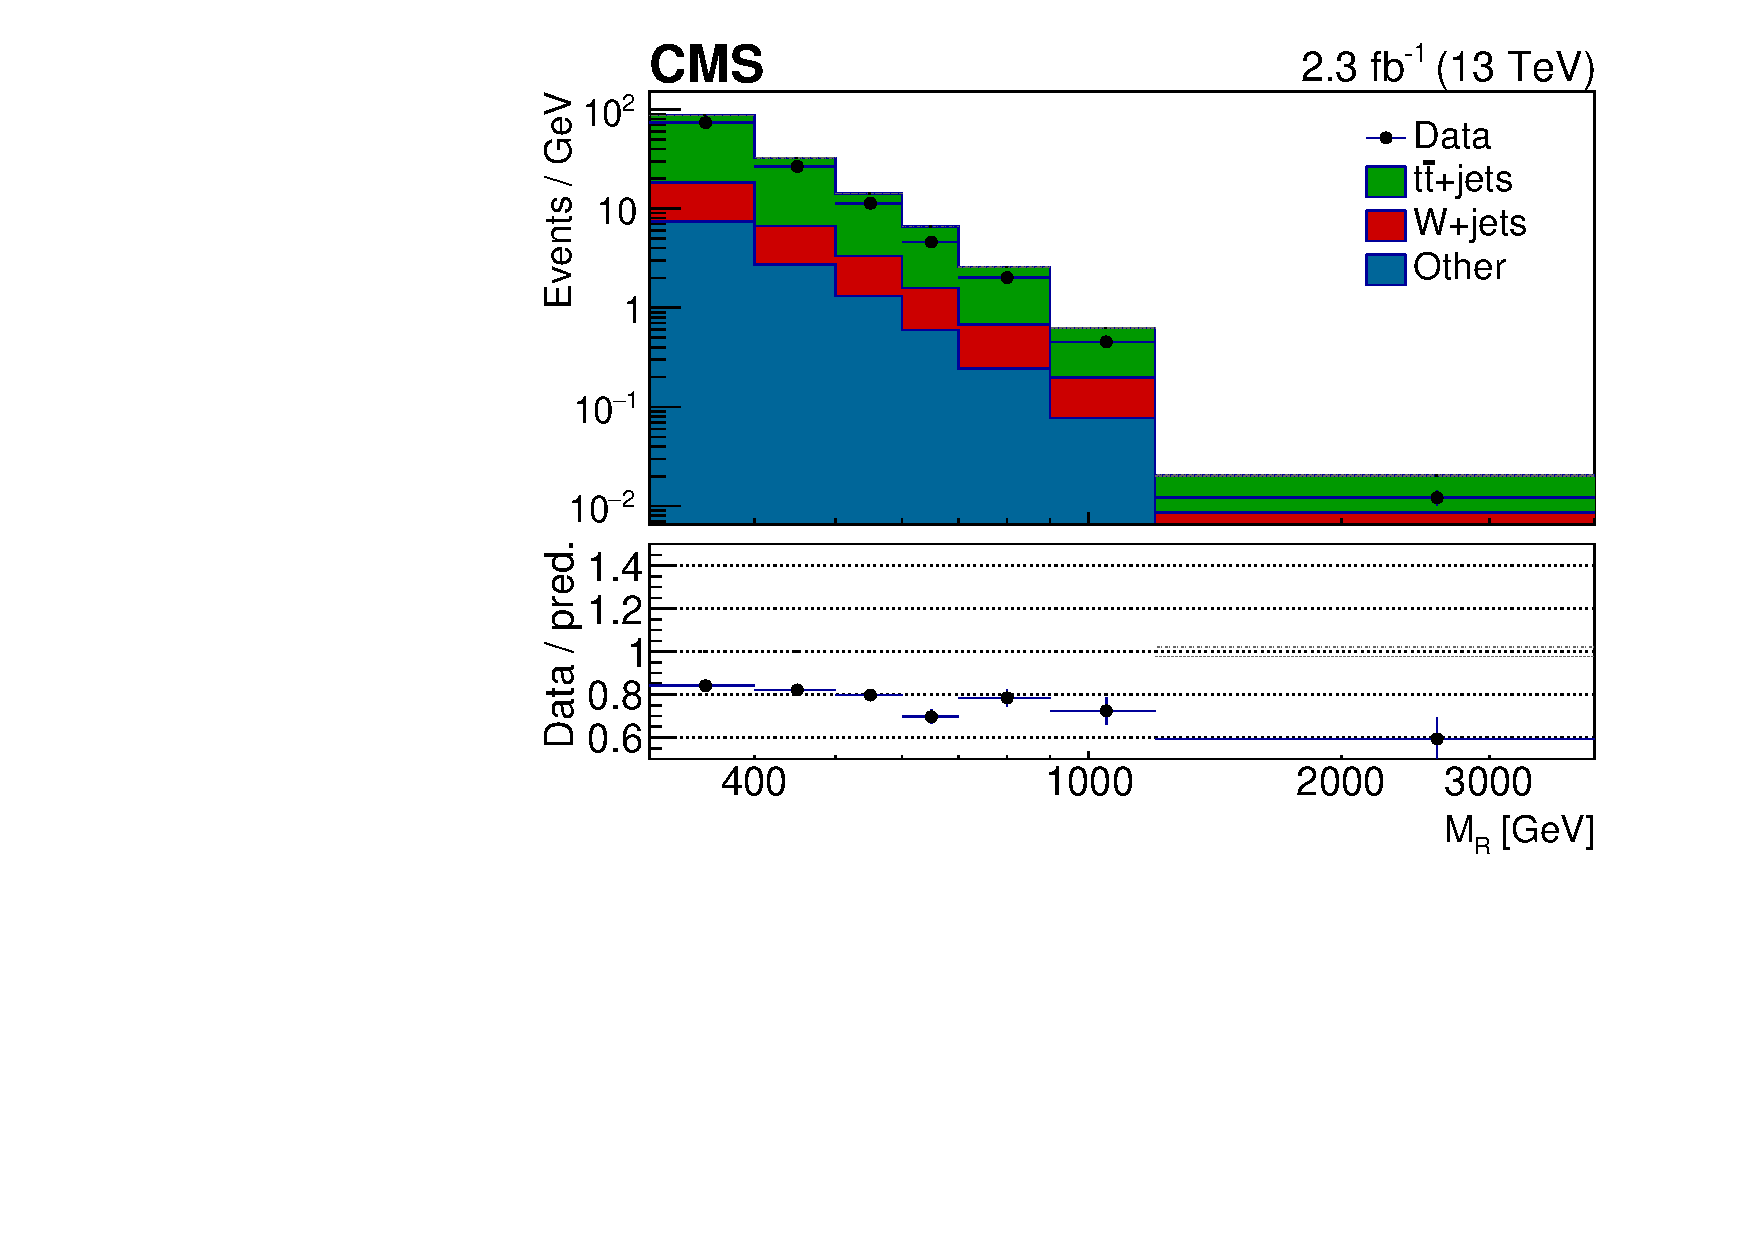
\includegraphics[width=0.45\textwidth]{figs/analysis13TeV/TTBarWJets/MR_TTJetsSingleLepton.pdf}
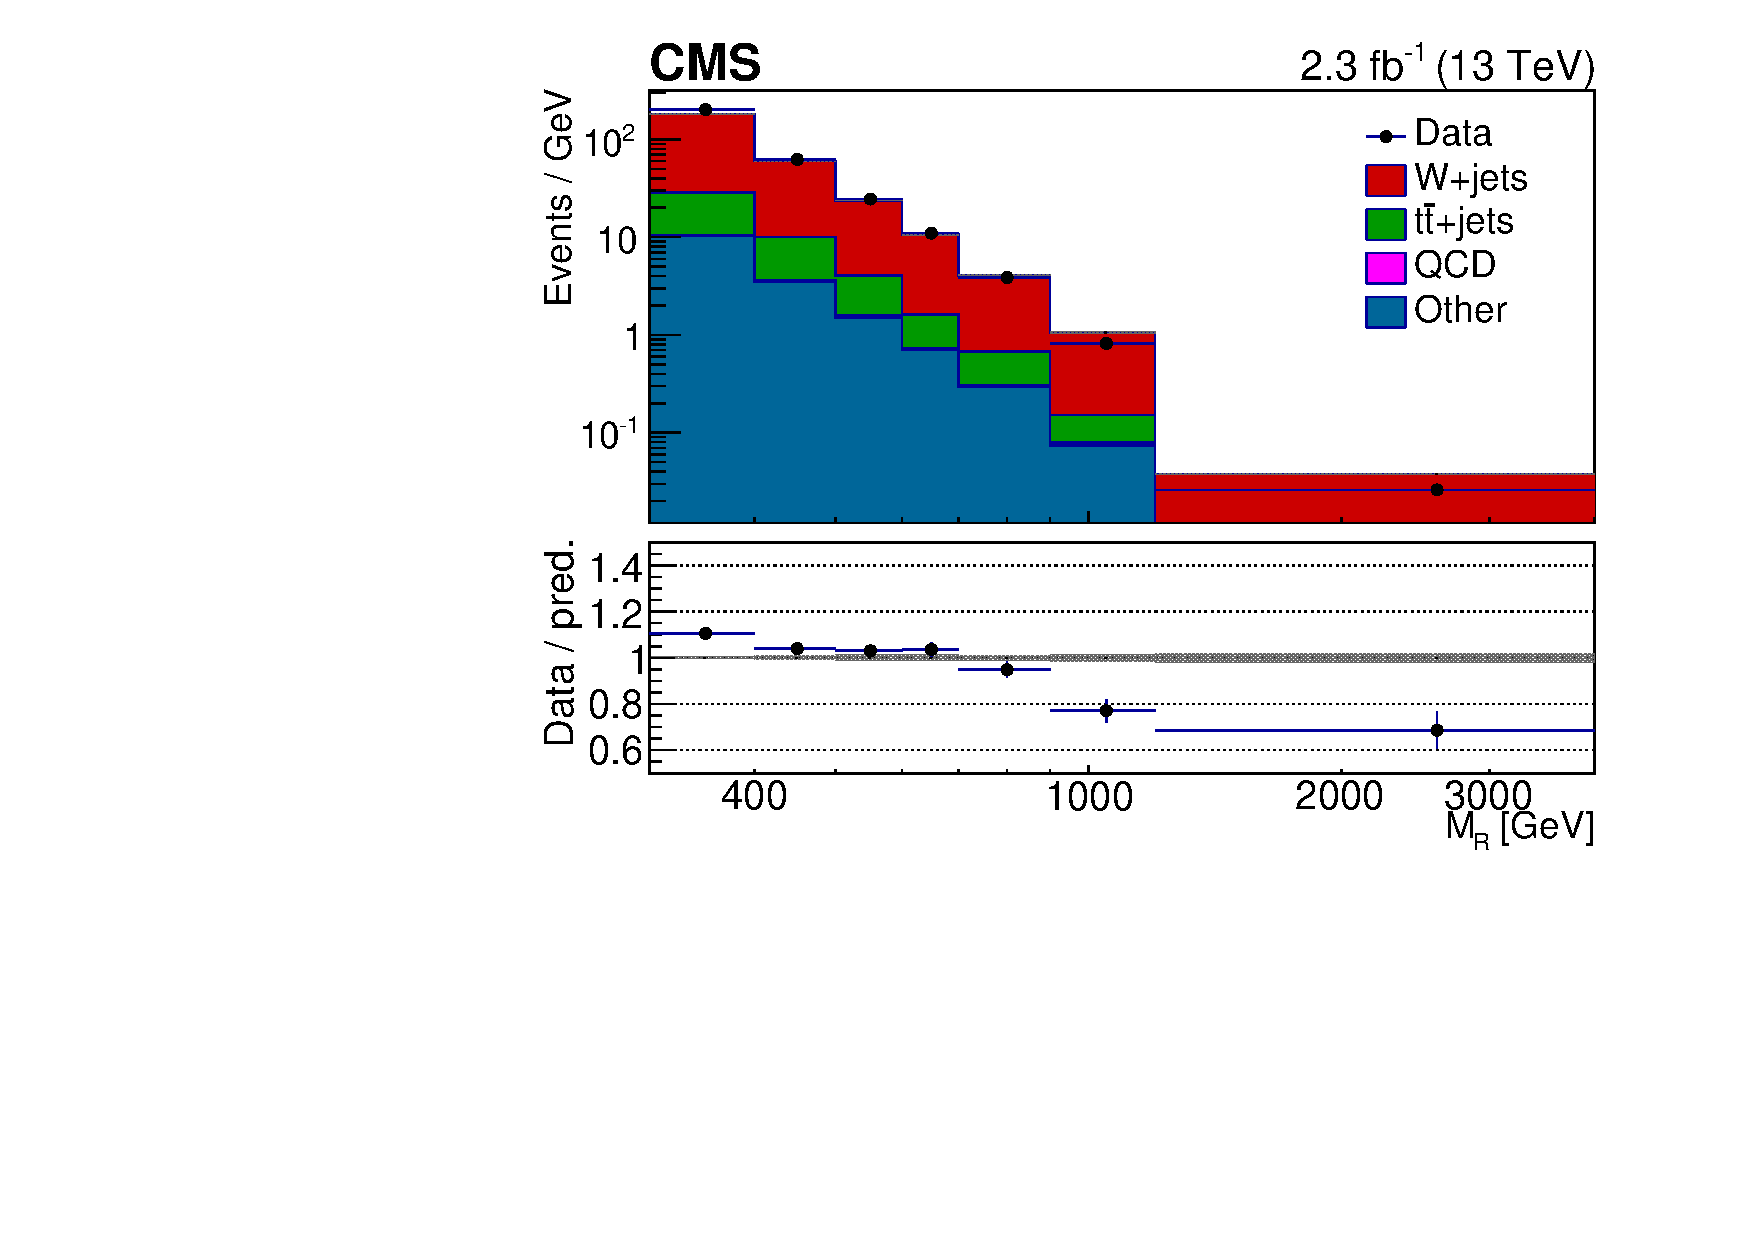
\includegraphics[width=0.45\textwidth]{figs/analysis13TeV/TTBarWJets/MR_WJetsSingleLepton.pdf}
\caption{ The $\MR$ distributions for events in the $\ttbar$ (left) and $\PW(\ell\nu)$+jets (right) 
control regions are shown, comparing data with the MC prediction.  In the right-hand plot, the $\ttbar$ MC events have been reweighted according to the corrections derived in the $\ttbar$ enhanced control region.  
 }
\label{fig:TTBarWJetsCR_MR}
\end{figure}

\begin{figure}[!htb] \centering
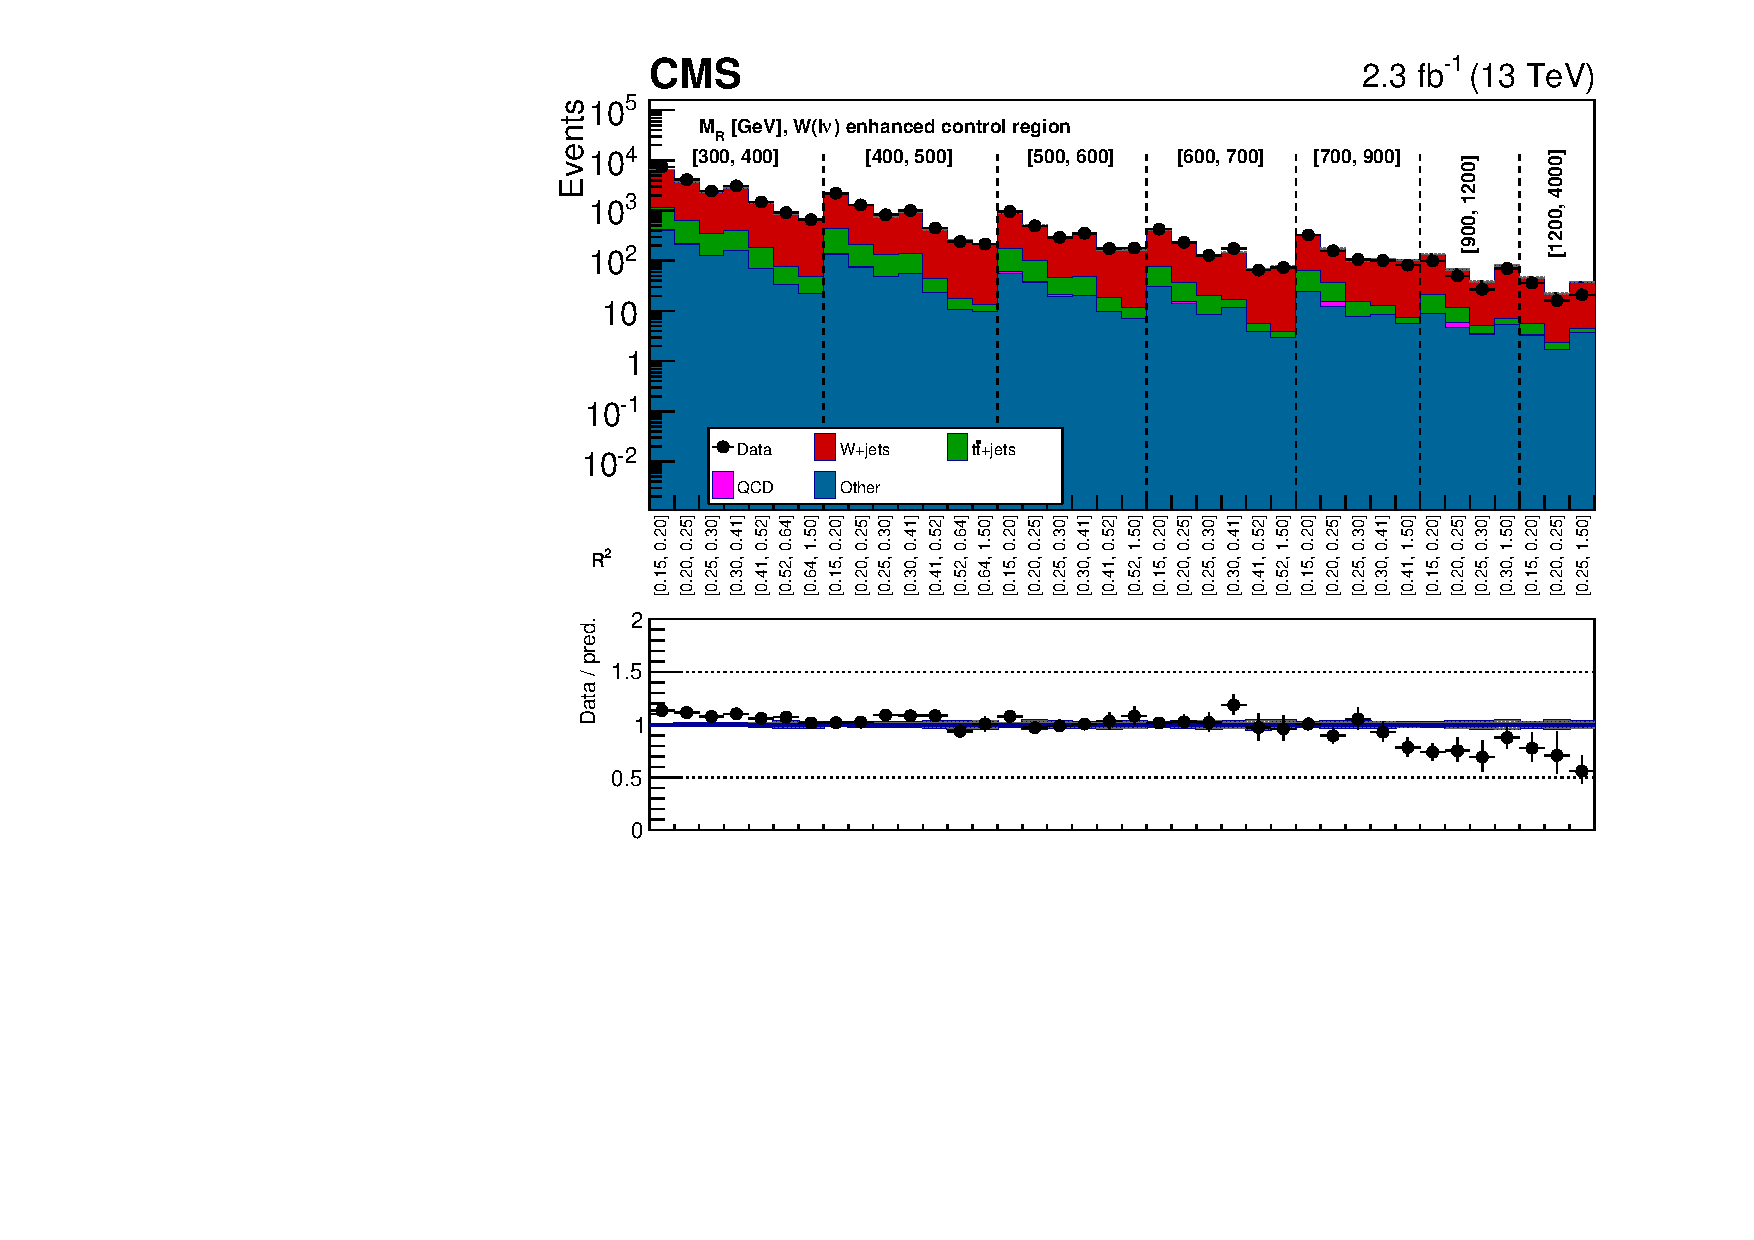
\includegraphics[width=0.95\textwidth]{figs/analysis13TeV/TTBarWJets/MRRsqWJetsSingleLeptonUnrolledDataMC.pdf}
\caption{ The two dimensional $\MR$ and $\Rtwo$ distribution for the $\PW(\ell\nu)$+jets enhanced control region 
is shown, comparing data with the MC prediction. The $\ttbar$ MC events in this control sample have been reweighted 
according to the corrections derived in the $\ttbar$ enhanced control region. The two dimensional $\MR$-$\Rtwo$ 
distribution is shown in a one dimensional representation, with each $\MR$ bin marked by the dashed lines and labeled near the top,
and each $\Rtwo$ bin labeled below. The ratio of data to the background prediction is shown on the bottom inset, with
the statistical uncertainty expressed through the data point error bars and the systematic uncertainty of the
background prediction represented by the shaded region. 
}
\label{fig:WJetsControlRegion_MRRsq_Unrolled}
\end{figure}

Corrections to the MC are first measured and applied as a function of $\MR$ and $\Rtwo$, inclusively in the
number of selected jets. As our search region requires a higher multiplicity of jets, an additional correction factor
is required to accurately model the jet multiplicity. We measure this additional 
correction factor to be $0.90 \pm 0.03$ by comparing the data and the MC prediction in the $\PW(\ell\nu)$+jets and $\ttbar$ 
control region for events with four or more jets.
To control for possible simulation mismodeling that is correlated between the number of jets and the razor
variables, we perform additional cross-checks of the $\MR$ and $\Rtwo$ distributions in bins of 
the number of \PQb-tagged jets in the $\ttbar$ and $\PW(\ell\nu)$+jets
control regions for events with four or more jets. For bins which show statistically significant disagreement,
the size of the disagreement is propagated as a systematic uncertainty. The typical range of these additional 
systematic uncertainties is between $10\%$ and $30\%$.

The $\ttbar$ and $\PW(\ell\nu)$+jets backgrounds in the zero lepton Multi-Jet event category are 
composed of events with at least one lepton in the final state, which is either out of 
acceptance or fails the veto electron, muon, or hadronic tau selection. 
Two additional control regions are defined in order to control the accuracy of the modeling of the 
acceptance and efficiency for selecting electrons or muons, and hadronic taus. 
We require events in the veto lepton (veto hadronic tau) control region to have at least one veto electron or muon
(hadronic tau) selected. The transverse mass is required to be between $30\GeV$ and $100\GeV$ in order to 
suppress QCD multijet background and contamination from potential new physics processes. At least two jets
with $\pt>80$~GeV and at least four jets with $\pt>40\GeV$ are required,
consistent with the search region requirements. Finally, we consider events with 
$\MR > 400$~GeV and $\Rtwo>0.25$. The distribution of the veto lepton $p_{T}$ for events in the veto 
lepton and veto hadronic tau control regions are shown in Figure~\ref{fig:VetoLeptonCR_LepPt},
and demonstrate that the MC models well the observed data.
The observed discrepancies in any bin are propagated as systematic uncertainties to the 
prediction of the $\ttbar$ and $\PW(\ell\nu)$+jets in the Multi-Jet category search region.

\begin{figure}[!htb] \centering
\subfigure[Veto Electrons or Muons]{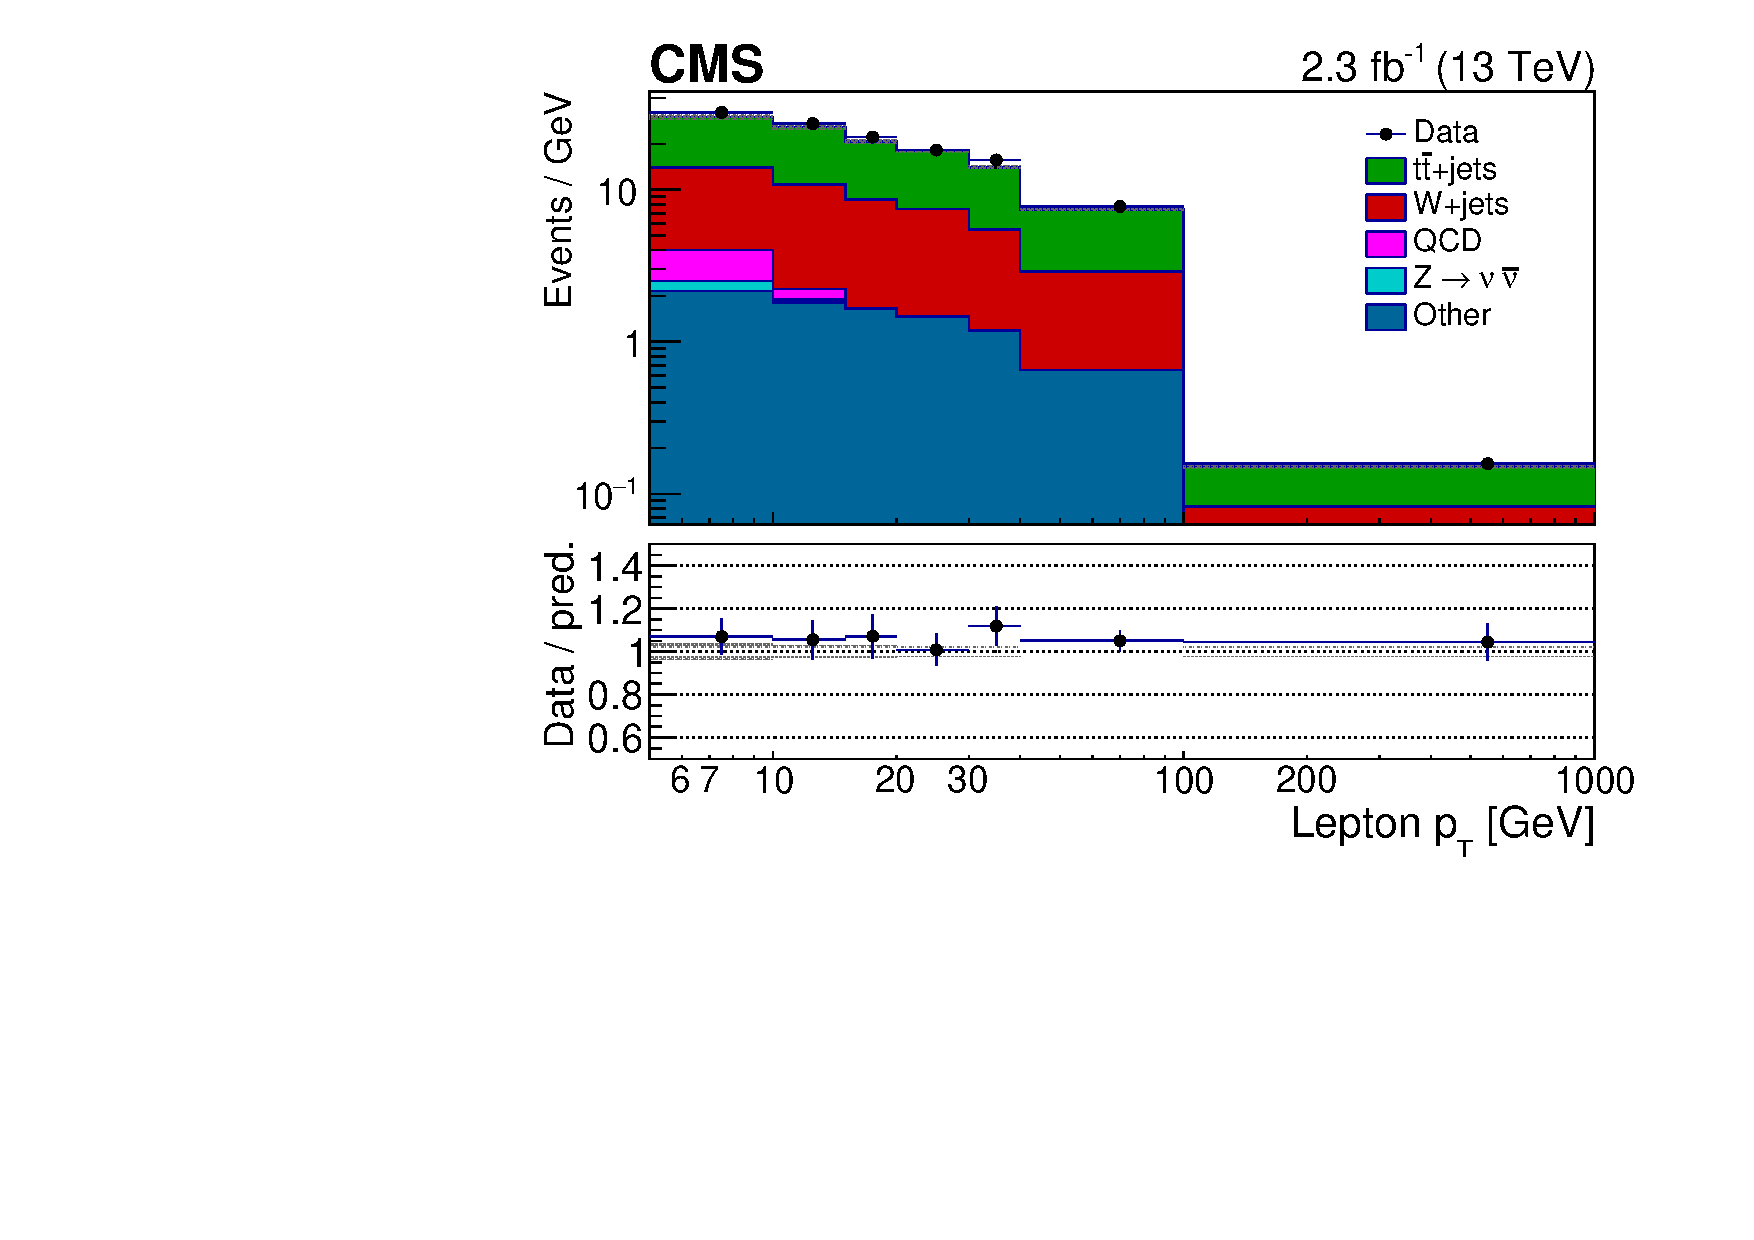
\includegraphics[width=0.49\textwidth]{figs/analysis13TeV/TTBarWJets/lep1Pt_VetoLeptonControlRegion_Density.pdf}}
\subfigure[Veto Hadronic Tau]{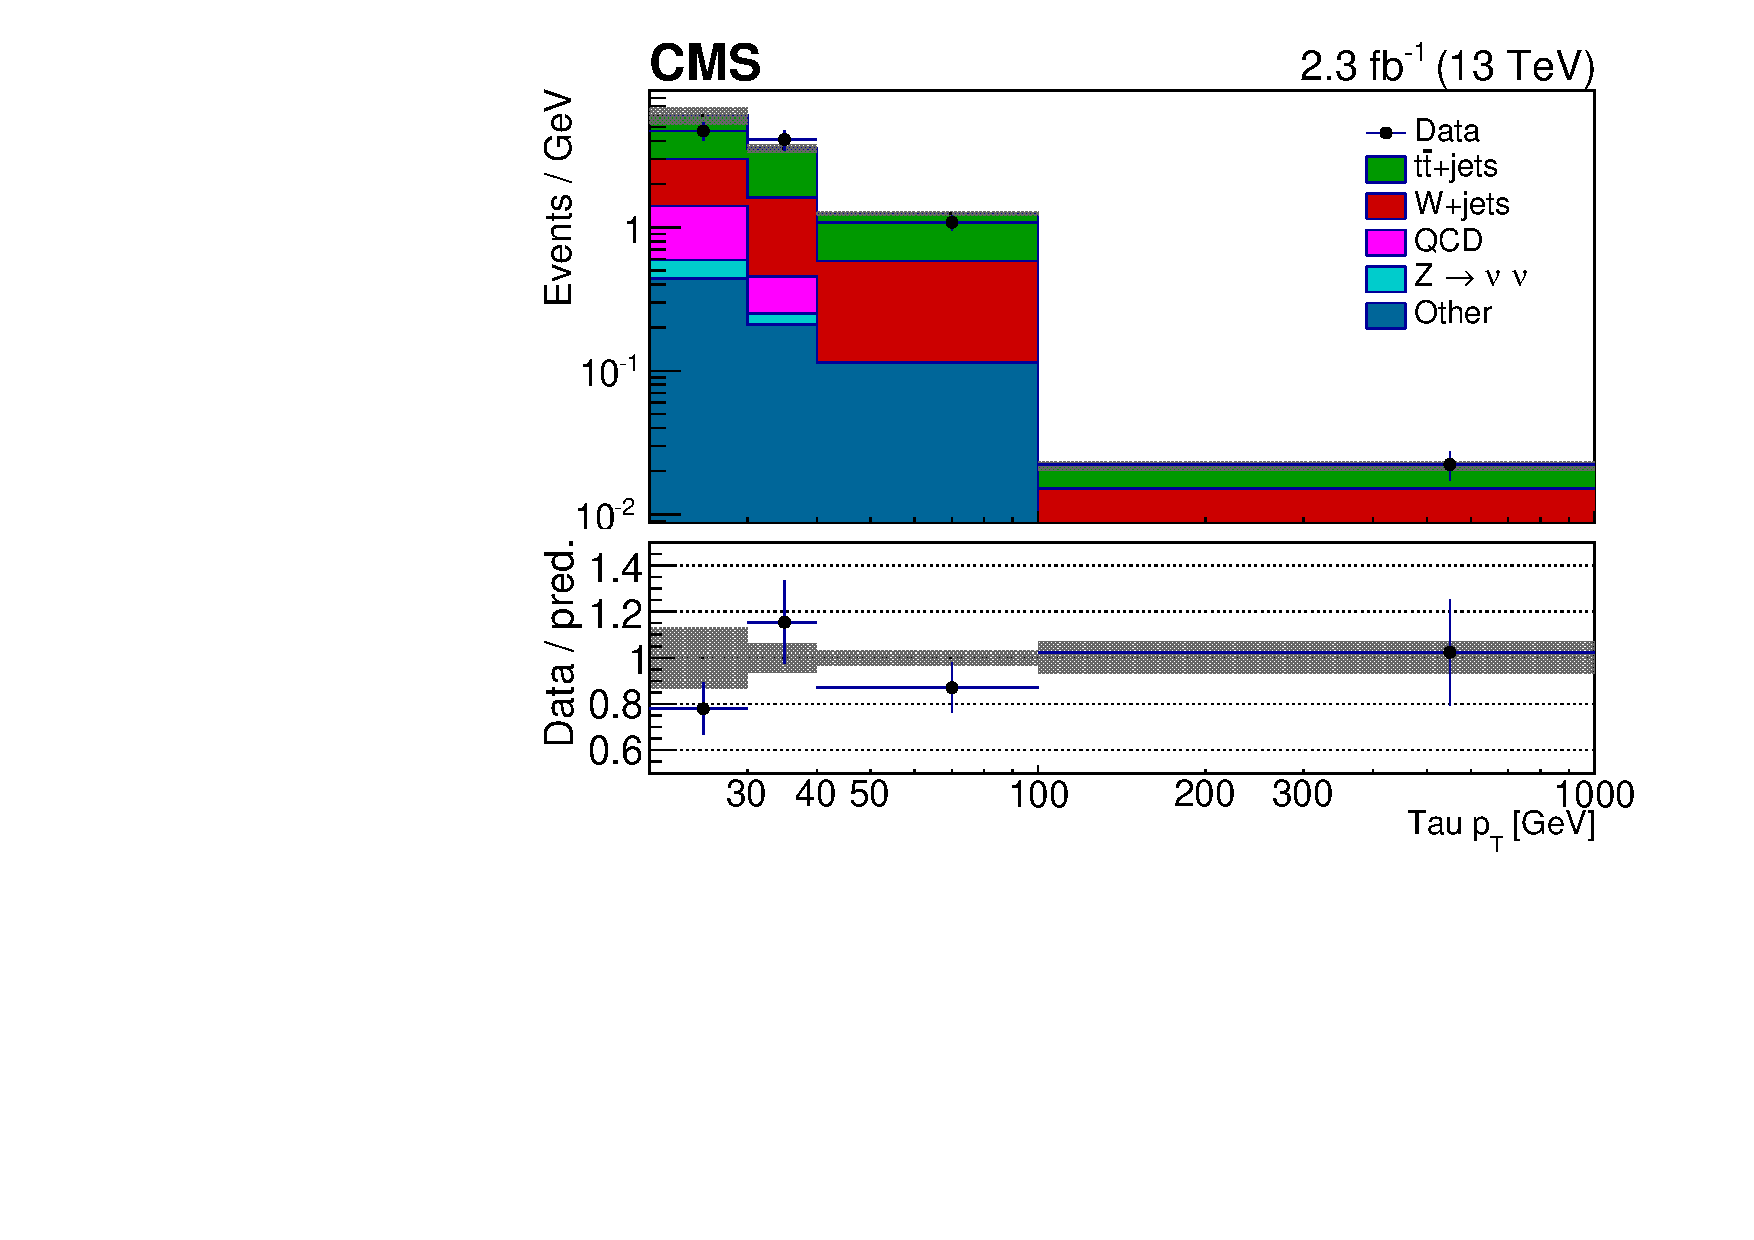
\includegraphics[width=0.49\textwidth]{figs/analysis13TeV/TTBarWJets/lep1Pt_VetoTauControlRegion_Density.pdf}}
\caption{ The $\pt$ distribution of the veto electron or muon (left) and the veto hadronic tau (right)
is shown for events in the veto lepton control regions, comparing data with the MC prediction. The $\ttbar$ and 
$\PW(\ell\nu)$+jets MC events have been reweighted according to the correction factors derived
in the $\ttbar$ enhanced and $\PW(\ell\nu)$+jets enhanced control regions, respectively.  
The event yields in each bin are normalized by the bin width. The ratio of data to the MC prediction
is shown in the bottom inset.
}
\label{fig:VetoLeptonCR_LepPt}
\end{figure}

The $\ttbar$ background in the Electron Multi-Jet and Muon Multi-Jet categories are primarily from
the dilepton decay mode as the transverse mass cut highly suppresses the semi-leptonic decay
mode. Corrections to the MC derived from the $\ttbar$ control region are primarily comprised
of semi-leptonic decays. We define an additional control region enhanced in dilepton $\ttbar$ decays 
to confirm that the MC corrections derived from a region dominated by
semi-leptonic decays also apply to dilepton decays. We select events with two tight leptons, 
both with $\pt>30 \GeV$, missing transverse energy above $40\GeV$, and 
dilepton mass larger than $20\GeV$. For events with two leptons of the same flavor, we additionally
veto events with dilepton mass between $76$ and $106\GeV$ in order to suppress background from $\cPZ$ 
decays. At least one \PQb-tagged jet is required to enhance the purity for the $\ttbar$
process. Finally, we mimic the phase space region similar to our search region in the Electron and
Muon Multi-Jet categories by simulating the failed identification of one of leptons and applying
the transverse mass cut using the other lepton. The correction factors measured in the 
$\ttbar$ control region are applied to the MC prediction of the dilepton
$\ttbar$ cross-check region in bins of $\MR$ and $\Rtwo$.
In Figure~\ref{fig:TTBarDileptonCR_MRRsqUnrolled}
we show the $\MR$-$\Rtwo$ distribution for the dilepton $\ttbar$ cross-check region
in events with four or more jets, and we observe no significant mismodeling by the MC, 
indicating that the measured corrections are accurate.

\begin{figure}[!htb] \centering
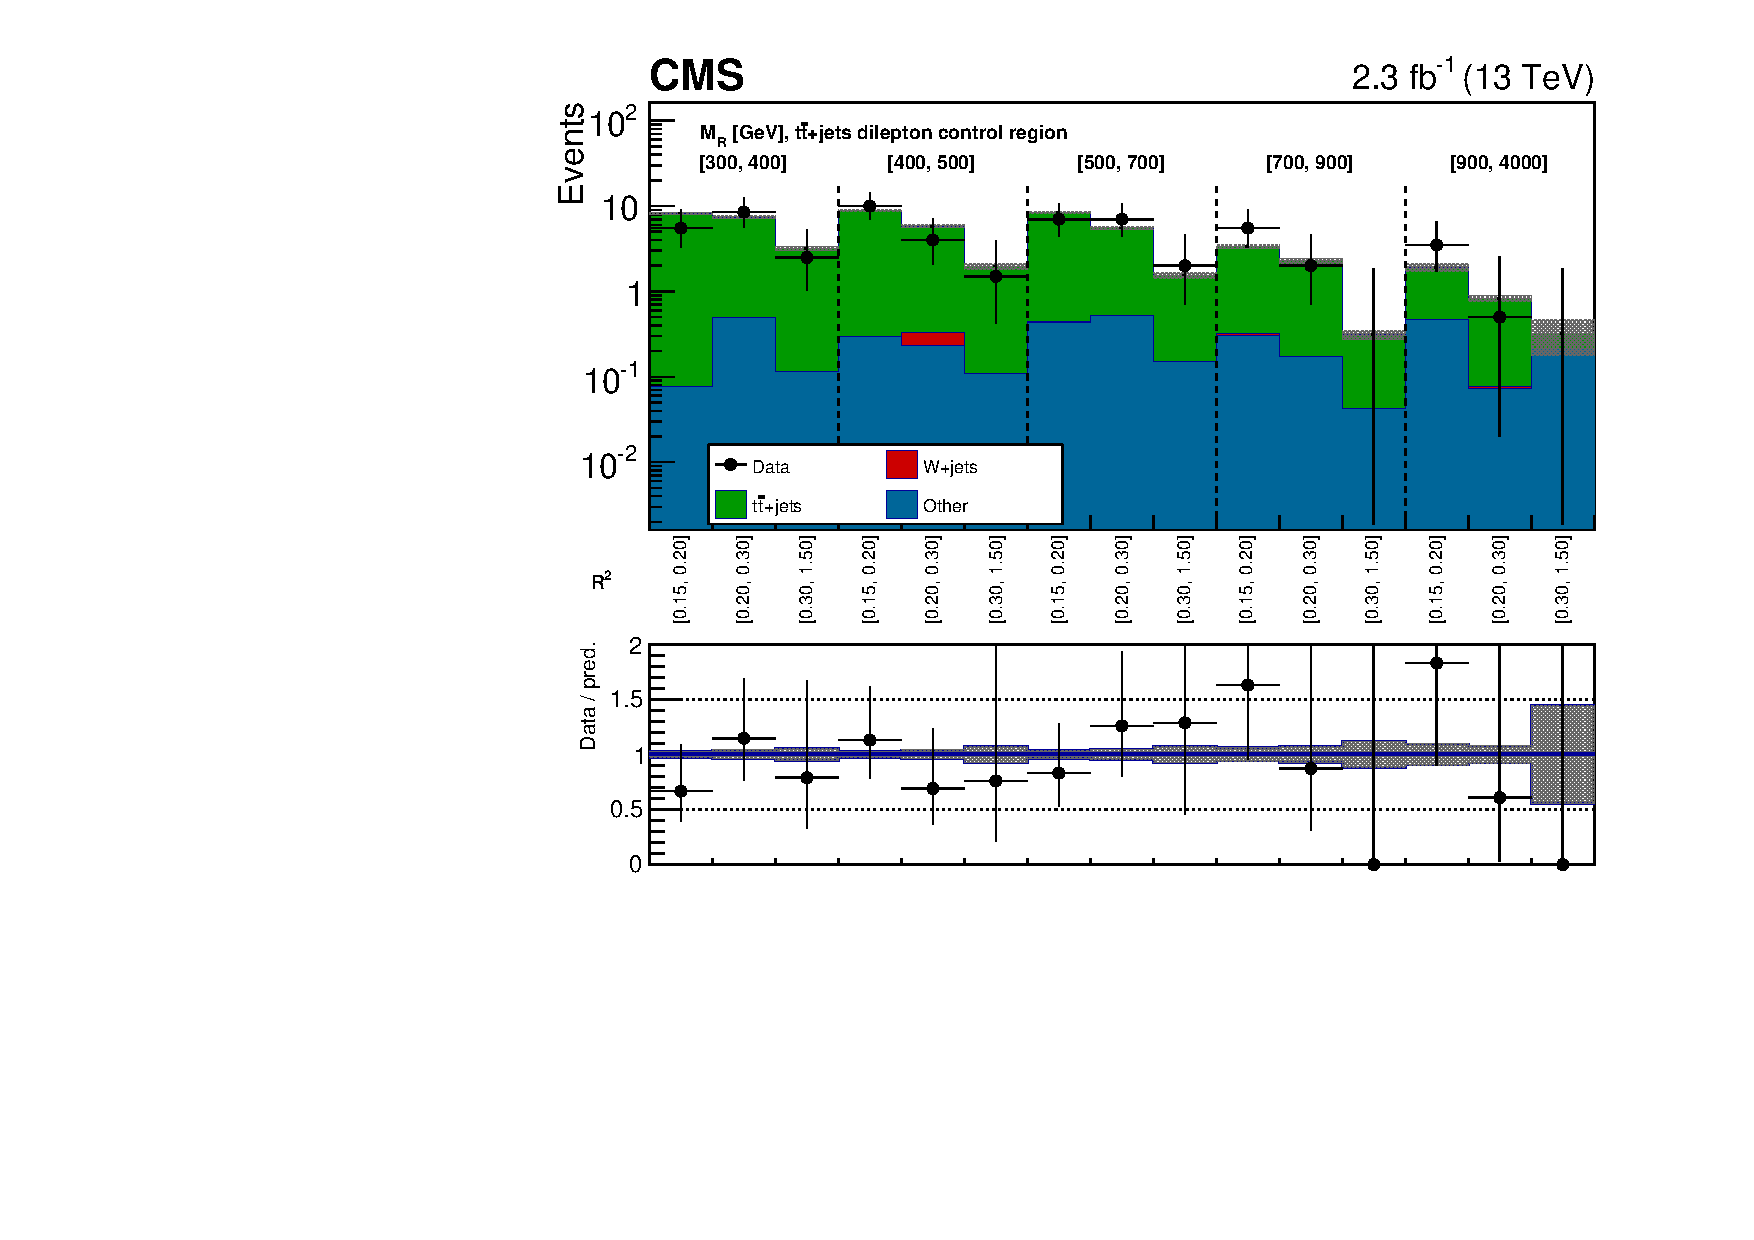
\includegraphics[width=0.95\textwidth]{figs/analysis13TeV/TTBarWJets/Razor_TTBarDileptonCrossCheckRegion_MRRsqUnrolled_MR300Rsq0p15_all_Logy.pdf}
\caption{ The two dimensional $\MR$-$\Rtwo$ distribution for the $\ttbar$ dilepton control region is shown, 
comparing data with the MC prediction. The $\ttbar$ MC events have been reweighted according to the correction factors
derived in the $\ttbar$ enhanced control region.  The two dimensional $\MR$-$\Rtwo$ distribution is shown
in a one dimensional representation, with each $\MR$ bin marked by the dashed lines and labeled near the top
, and each $\Rtwo$ bin labeled below. The ratio of data to the background prediction is shown on the bottom inset, with
the statistical uncertainty expressed through the data point error bars and the systematic uncertainty of the
background prediction represented by the shaded region. 
}
\label{fig:TTBarDileptonCR_MRRsqUnrolled}
\end{figure}

\subsubsection{$\cPZ\to\nu\bar\nu$ Background}
\label{sec:ZInvCR}
Three independent control regions are used to predict the $\cPZ(\nu\bar\nu)$+jets background,
relying on the assumption that the hadronic recoil spectrum and the jet multiplicity distribution
of the $\cPZ(\nu\bar\nu)$+jets process are similar to those of the $\PW(\ell\nu)$+jets and $\cPgg$+jets 
processes. The primary and most populated control region is the $\cPgg$+jets control region, 
defined by selecting events with at least one photon passing loose identification and
isolation requirements. The events are triggered using single photon triggers, and 
the photon is required to have $\pt>50\GeV$. The momentum of the photon candidate
in the tranverse plane is added vectorially to $\ptvecmiss$ 
in order to simulate an invisible particle, as one would have in the case of a 
$\cPZ\to\nu\bar\nu$ decay, and the $\MR$ and $\Rtwo$ variables are computed according to
this invisible decay scenario. The requirements on $\MR$ and $\Rtwo$ sculpts the
photon $\pt$ distribution, which turns on starting around $120\GeV$ and peaks at around
$200\GeV$.  A template fit to the distribution of $\sigma_{i \eta i \eta}$ is 
performed to determine the contribution from misidentified photons to the $\cPgg$+jets 
control region and is found to be about $5\%$, independent of $\MR$ and $\Rtwo$. 
Events from the $\cPgg$+jets process where the photon is produced within the cone of a jet
(labeled as $\cPgg$+jets fragmentation) are considered to be background and subtracted
using the MC prediction. Backgrounds from rarer processes such as $\PW\cPgg$, $\cPZ\cPgg$, 
and $\ttbar\cPgg$ are also subtracted using the MC prediction.
In Figure~\ref{fig:Znn_PhotonJets}, we show the $\MR$ distribution as well as the two
dimensional $\MR$-$\Rtwo$ distribution for the $\cPgg$+jets control region, where we again 
observe a steeper $\MR$ falloff in the data compared to the MC. Correction factors 
are derived in bins of $\MR$ and $\Rtwo$ and applied to the MC prediction for the 
$\cPZ\to\nu\bar\nu$ background in the search region. The statistical uncertainties for the 
correction factors range between $10\%$ and $30\%$ and are one of the dominant uncertainties
for the $\cPZ\to\nu\bar\nu$ background prediction. 
Analogous to the procedure for the $\ttbar$ and $\PW(\ell\nu)$+jets control region, we derive an additional correction
factor of $0.87 \pm 0.05$ to accurately describe the yield in events with four or more jets. Additional
cross-checks are performed in bins of the number of b-tagged jets and systematic uncertainties ranging
from $4\%$ for events with zero b-tagged jets to $58\%$ for events with three or more b-tagged jets are
derived.

\begin{figure}[!htb] \centering
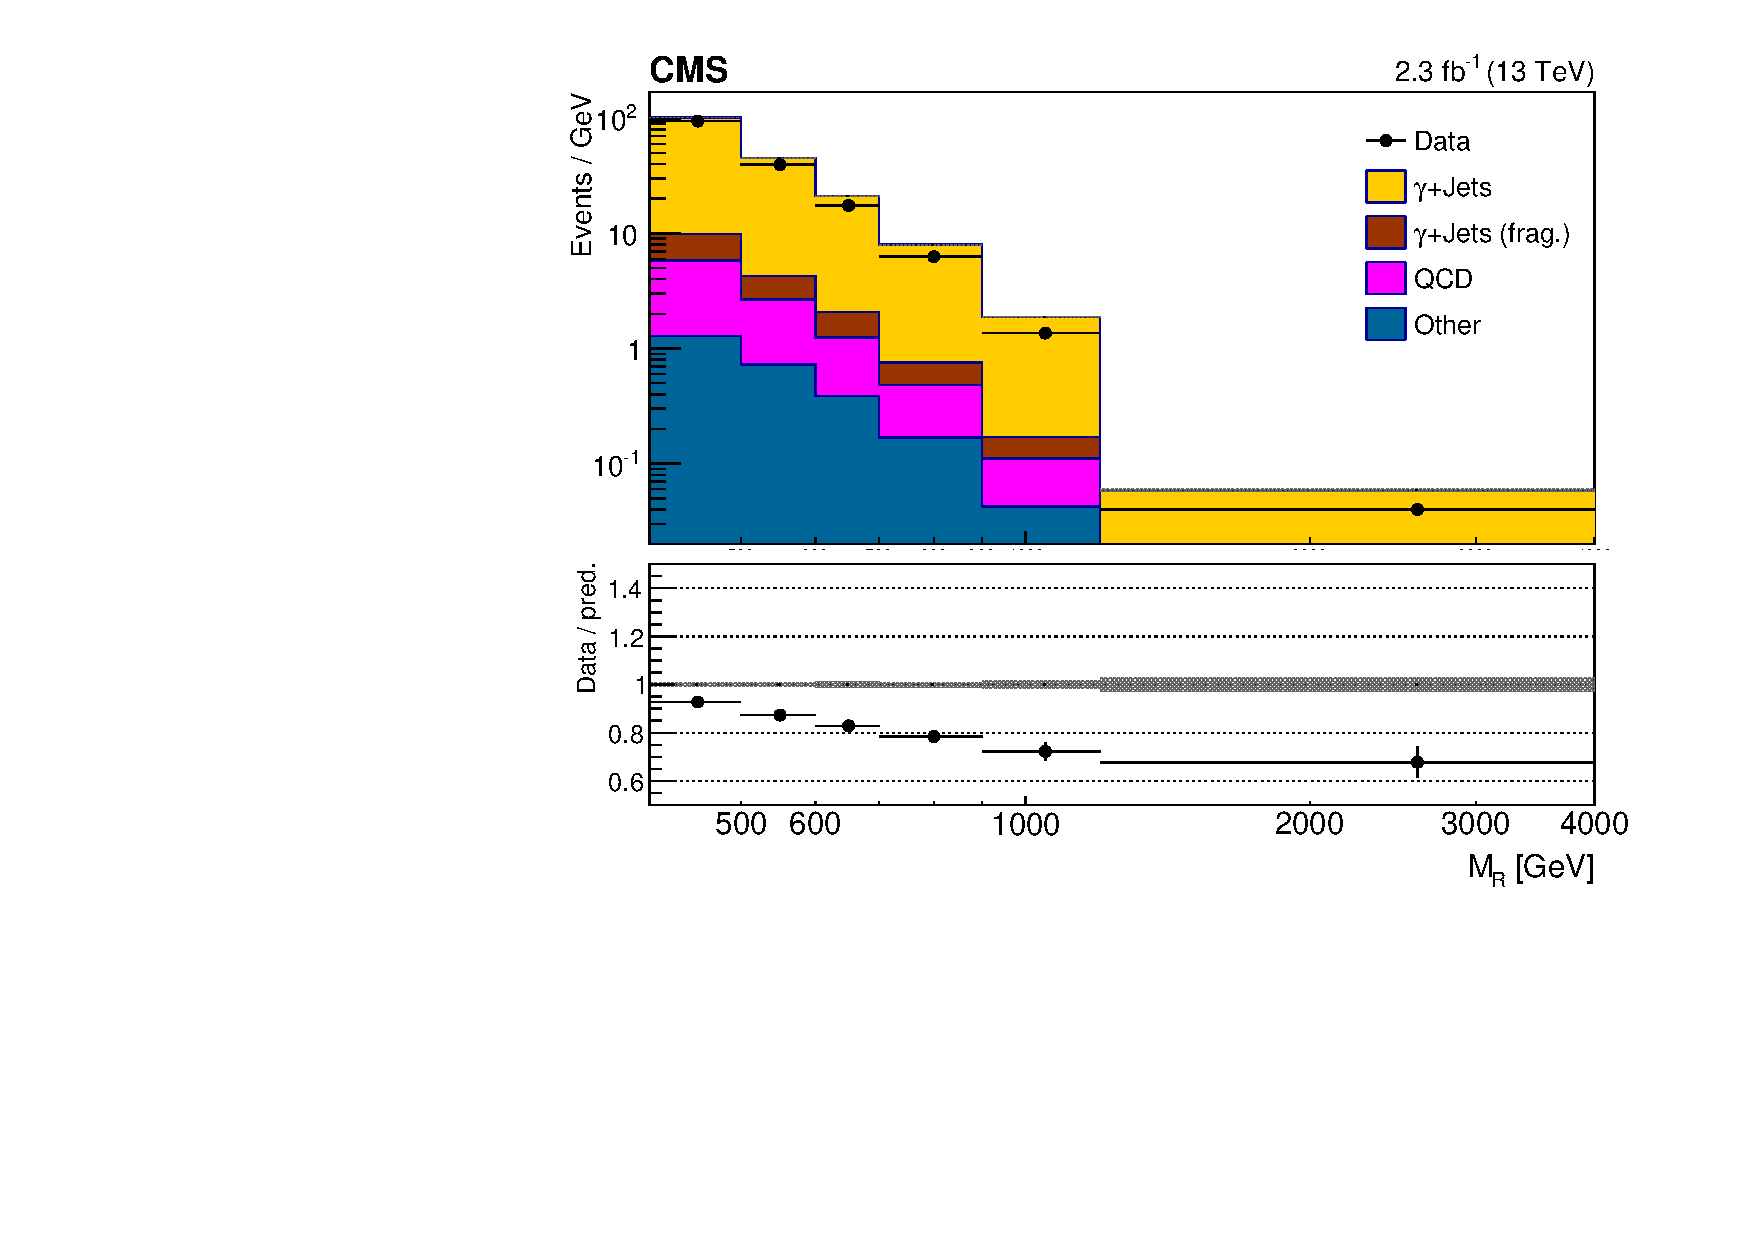
\includegraphics[width=0.55\textwidth]{figs/analysis13TeV/Znunu/Razor_PhotonControlRegion_MR_PhotonCR_Logy.pdf} \\
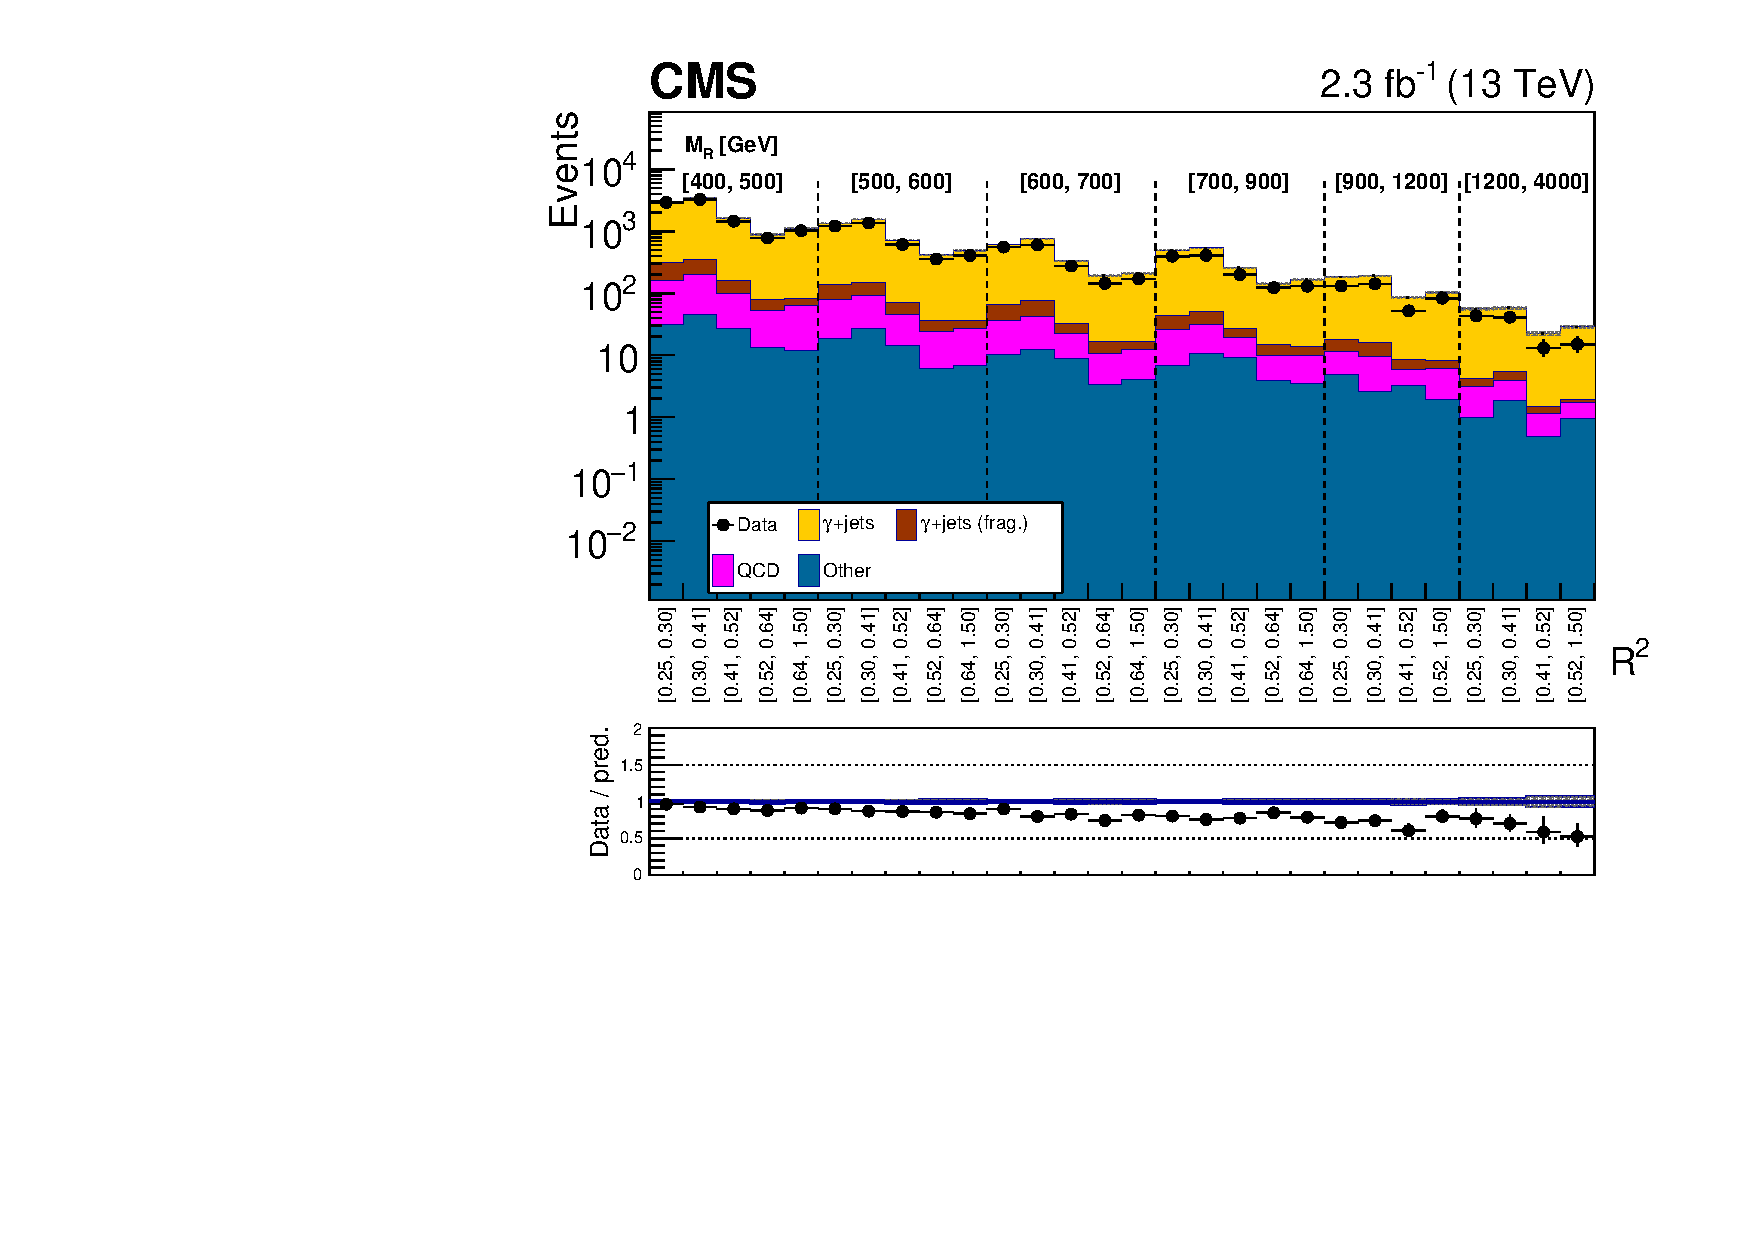
\includegraphics[width=0.95\textwidth]{figs/analysis13TeV/Znunu/Razor_PhotonControlRegion_MRRsqUnrolled_PhotonCR_Logy.pdf}
\caption{The one-dimensional distribution of $\MR$ in the $\cPgg$+jets control region
  (above) and the two-dimensional $\MR$-$\Rtwo$ distribution in
  the $\cPgg$+jets control region (below) are shown. The two dimensional $\MR$-$\Rtwo$ distribution is shown
in a one dimensional representation, with each $\MR$ bin marked by the dashed lines and labeled near the top,
and each $\Rtwo$ bin labeled below. The ratio of data to the background prediction is shown on the bottom inset, with
the statistical uncertainty expressed through the data point error bars and the systematic uncertainty of the
background prediction represented by the shaded region. 
} 
\label{fig:Znn_PhotonJets}
\end{figure}


The second control region, enhanced in $\PW(\ell\nu)$+jets, is defined identically to the $\PW(\ell\nu)$+jets control region described
above in Section~\ref{sec:TTBarWJetsCR}, except that the lepton is treated as invisible
by adding its momentum vectorially to $\ptvecmiss$ and the $\MR$ and $\Rtwo$
variables are computed accordingly. Correction factors are computed using events from this control region,
and the difference between these correction factors and those computed from the $\cPgg$+jets control region
is propagated as a systematic uncertainty.  These uncertainties range between $10\%$ and $40\%$ depending on the $\MR$-$\Rtwo$ bin. 

The third control region, enhanced in $\cPZ\to\ell^+\ell^-$ decays, 
is defined by selecting events with two tight electrons or two tight muons, and requiring that the dilepton mass is
between $76\GeV$ and $106\GeV$. Events are required to have no \PQb-tagged jets
in order to suppress $t\bar{t}$ background. The two leptons are treated as invisible by adding their
momenta vectorially to $\ptvecmiss$. We apply the correction factors obtained from the
$\cPgg$+jet control region to the $\cPZ\to\ell^+\ell^-$ MC prediction and perform a cross-check against data
in this control region. No significant discrepancy between the data and the prediction is observed.

\subsubsection{QCD Multijet Background}
\label{sec:QCDCR}
The QCD multijet process contributes about $10\%$ of the total background in the zero lepton Multi-Jet
event category for bins with zero or one \PQb-tagged jets. Such events enter the search regions
in the tails of the missing transverse energy distribution when the energy of 
one of the jets in the event is significantly under- or over-measured. 
In most such situations, the missing transverse momentum points either toward
or away from the leading jets and therefore the two megajet hemipsheres tend to
be in a back-to-back configuration. Our search region is defined by requiring that
the azimuthal angle between the two megajet hemispheres $\Delta\phi_R$ is less than
$2.8$. We define the control region for the QCD background process to be events
with $\dPhiR>2.8$, keeping all other selection requirements identical to those for
the search region. The purity of the QCD multijet process in the control region
is more than $70\%$. After subtracting for non-QCD background,
we project the observed data yield in the control region to the search region using
the translation factor $\zeta$:

\begin{equation}
\zeta = \frac{N(|\dPhiR|>2.8)}{N(|\dPhiR|<2.8)}.
\end{equation}

We find that the translation factor calculated from the MC
decreases as a function of $\MR$ and is, to a large degree, constant as a function of $\Rtwo$.
Using data events in the low $\Rtwo$ region ($0.15$ to $0.25$), dominated
by QCD multijet background, we measure the translation factor $\zeta$ as a function of
$\MR$ to cross-check the values obtained from the MC.
The $\MR$ dependence of $\zeta$ is modeled as the sum of a power law and constant.  
This functional shape is fitted to the values of $\zeta$ calculated from the MC.
A systematic uncertainty of $87\%$ is propagated, covering both the difference
between the values measured in MC and data and the spread around the
fitted model as a function of $\MR$ and $\Rtwo$ in MC. The function used
for the translation factor $\zeta$ and the values measured in data and MC are
shown in Figure~\ref{fig:QCDTranslationFactor}. 

\begin{figure}[!htb]
\begin{center}
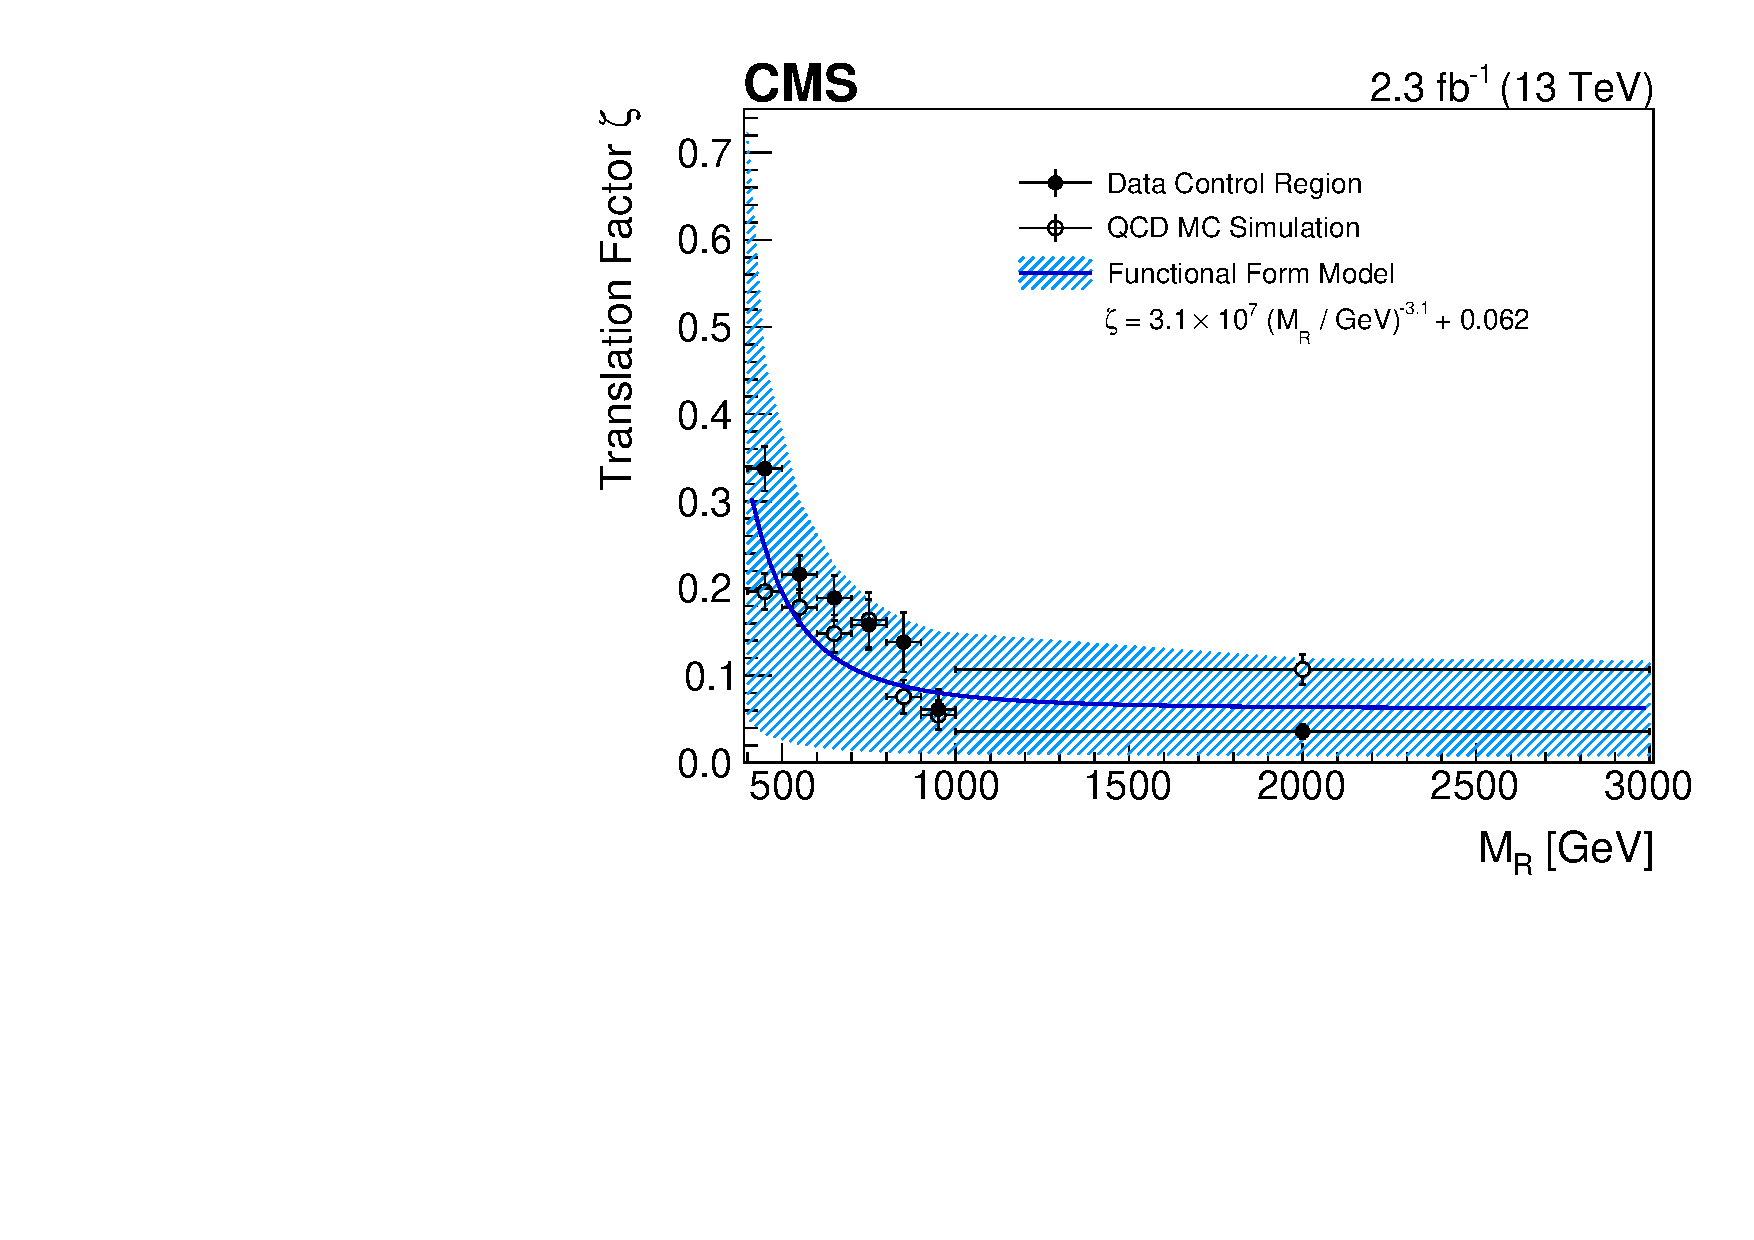
\includegraphics[width=0.75\textwidth]{figs/analysis13TeV/npf_vs_mr_razor_fit.pdf}
\caption{\label{fig:QCDTranslationFactor} 
The translation factor $\zeta$ is shown as a function of $\MR$. The curve shows the 
functional form used to model the $\MR$ dependence, and the open circle and black square data
points are the values of $\zeta$ measured in the low $\Rtwo$ data control region and the QCD MC
respectively. The hashed region indicates the size of the systematic uncertainty on
$\zeta$.
}
\end{center}
\end{figure}

We perform two additional cross-checks on the accuracy of the MC prediction for
$\zeta$ in control regions dominated by processes similar to the QCD multijet
background with no invisible neutrinos in the final state. The first 
cross-check is performed on a dimuon control region enhanced in $\cPZ\rightarrow\Pgm^+\Pgm^-$ decays, 
and the second cross-check is performed on a dijet control region enhanced in QCD dijet events. 
In both cases, the events at large $\Rtwo$ result from cases similar to our search region
where the energy of a leading jet is pathologically mismeasured. We compare the values of
$\zeta$ measured in these data control regions to the values predicted by the MC
and observe agreement at the $20\%$ level, well within the 
systematic unceratinty of $87\%$ assigned to our QCD background estimate. 


\subsection{Method B: Fit-based Background Prediction}
\label{sec:FitBkg}

The second background prediction method is based on a fit to the data with an 
assumed functional form for the shape of the background distribution in the $\MR$-$\Rtwo$ plane. 
Based on past studies~\cite{razorPRD,razor8TeV}, the shape of the background in
the $\MR$ and $\Rtwo$ variables is found to be well described by the following functional form:

\begin{equation}
 f_{\mathrm{SM}}(\MR,\Rtwo) =  \bigl[b(\MR-{\MRz})^{1/n}(\Rtwo-{\Rtwoz})
  ^{1/n}-1\bigr]\re^{-bn(\MR-{\MRz})^{1/n}(\Rtwo-{\Rtwoz})
    ^{1/n}} .
\label{eq:razFunction}
\end{equation}

The shape is described by four parameters: $\MRz$, $\Rtwoz$, $b$, and $n$. 
The two parameters $b$ and $n$ determine the tail of the distribution in the 
two-dimensional plane, while the $\MRz$ ($\Rtwoz$) parameter affects the tail of the 
one-dimensional projection on $\Rtwo$ ($\MR$). For $n=1$, the function 
projects to an exponential both on $\Rtwo$ and $\MR$, and $b$ is
proportional to the exponential rate parameter in each one-dimensional
projection. 

Background estimation is performed using an extended, binned, maximum-likelihood fit to the $\MR$ and $\Rtwo$
distribution in one of two ways: 

\begin{itemize}
  \item A fit to the data in the sideband regions in $\MR$ and 
    $\Rtwo$, defined more precisely below, as a model-independent way to look for excesses or 
    discrepancies. The fit is performed using only the data in the 
    sideband, and the functional form is extrapolated to the full $\MR$ and $\Rtwo$ plane.
  \item A fit to the data in the full search region in $\MR$ and $\Rtwo$ under  
    background-only and signal-plus-background hypotheses, following 
    a modified frequentist approach (LHC $\CLs$)~\cite{Read:2002hq,Read:2000ru,Cowan:2010js,ATLAS:2011tau} 
    to interpret the data in the context of particular SUSY simplified models. 
\end{itemize}

The sideband region is defined to be $100 \GeV$ in width in $\MR$
and $0.05$ in $\Rtwo$. Explicitly, for the
Multi-Jet event category, it comprises the region $500 \GeV$
$< \MR < 600 \GeV$ and $\Rtwo > 0.3$, plus the region $\MR > 500 \GeV$
and $0.25 < \Rtwo < 0.3$.  For the Muon Multi-Jet and Electron Multi-Jet
event categories, it comprises the region $400 \GeV < \MR < 500 \GeV$
and $\Rtwo > 0.2$, plus the region $\MR > 400 \GeV$ and
$0.15 < \Rtwo < 0.2$. 

For each event category, we fit the two-dimensional distribution of 
$\MR$ and $\Rtwo$ in the sideband region using the
above functional form, separately for events with no \PQb-tagged jets, one
\PQb-tagged jet, two \PQb-tagged jets, and three or more \PQb-tagged jets. The
normalization in each event category and each \PQb-tagged jet bin is
independently varied in the fit. Due to the lack of data events in the category
with three or more \PQb-tagged jets, we constrain
the shape of this category to be related to the shape for events with two
\PQb-tagged jets as follows:
\begin{equation}
  f^{\geq 3\cPqb}_{\mathrm{SM}}(\MR, \Rtwo)  = (1+m_{\MR}(\MR - M^{\mathrm{offset}}_R))f^{2\cPqb}_{\mathrm{SM}}(\MR, \Rtwo),
\label{eq:3btagFunction}
\end{equation}
where $f^{2\cPqb}_{\mathrm{SM}}(\MR, \Rtwo)$ and $f^{\geq 3\cPqb}_{\mathrm{SM}}(\MR, \Rtwo)$ are the
probability density functions for events with
two \PQb-tagged jets and with three or more \PQb-tagged jets,
respectively; $\MR^{\mathrm{offset}}$ is the lowest $\MR$ value in a particular
event category; and $m_{\MR}$ is a floating parameter constrained by a Gaussian distribution
centered at the value measured using the MC and with a
100\% uncertainty. The above form for the shape of the background events 
with three or more \PQb-tagged jets was verified in MC.

Numerous tests were performed to establish the robustness of the fit
model in adequately describing the underlying distributions. To
demonstrate that the background model gives an accurate description of the 
background distributions, we construct a representative
data set using MC samples, and perform the background fit using
the functional form from Eq.~\ref{eq:razFunction}. Goodness-of-fit is
evaluated by comparing the background prediction from the fit with the
prediction from the MC. This procedure is performed
separately for each of the search categories and we find
that the fit function yields an accurate representation of the
background predicted by the MC.

We also observe that the fit model is insensitive to variations of the background
composition predicted by the MC in each event category by altering
relative contributions of the dominant backgrounds, performing a
new fit with the alternative background composition, and comparing
the new fit results to the nominal fit result. The contributions
of the main $\ttbar$, $\PW(\ell\nu)$+jets, and $\cPZ(\nu\bar\nu)$ backgrounds 
were varied by 30\%, and the rare backgrounds from QCD multijet and $\ttbar\cPZ$ 
were varied by 100\%. For the Muon Multi-Jet and Electron Multi-Jet event categories,
we also varied the contributions from the dileptonic and semi-leptonic decays
of the $\ttbar$ background separately by 30\%. In each of these tests, we 
observed that the chosen functional form can adequately describe the shapes of 
the $\MR$ and $\Rtwo$ distributions as predicted by the modified MC.

Additional pseudo-experiment studies were performed comparing the background prediction
from the sideband fit and the full region fit to evaluate the average
deviation between the two fit predictions. We observe that 
the sideband fit and the full region fit predictions in the
signal-sensitive region differ by up to 15\% and we propagate an
additional systematic uncertainty to the sideband fit background
prediction to cover this average difference.

%The best fit background
%shape is used as a probability density function and sampled to
%obtain an ensemble of toy experiments. For each toy experiment,
%we perform a sideband fit and a full region fit, and the fit predictions
%for the background yield in the region at high $M_{R}$ and high $R^{2}$ 
%are compared on a toy-by-toy basis. For the zero lepton category,
%the region is defined as $M_{R}>700 \GeV$ and $R^{2}>0.41$, while
%for the one lepton categories, the region is defined as 
% $M_{R}>500 \GeV$ and $R^{2}>0.25$. 
%Based on an ensemble of peusdo-experiments in which we sample a
%background-only pseudo-data set and then perform both a sideband fit
%and a full region fit, we observe that on average the sideband fit
%predicts a slightly smaller background yield in the signal-sensitive
%region compared to the full region fit and that the average relative
%difference decreases with increasing integrated luminosity.
%For the Multi-Jet category, the average difference decreases
%from about 15\% for data samples corresponding to $2 \fbinv$
%to less than 2\% for data samples corresponding to about $20 \fbinv$,
%while for the one-lepton categories, the average difference
%decreases from about 15\% to about 7\%. The average difference is small 
%compared to the total systematic uncertainty, which ranges from 40\%
%to 100\% depending on the \PQb-tag bin. Nonetheless, we propagate an
%additional systematic uncertainty to the sideband fit background
%prediction to cover these average differences.

\begin{figure}[!htb] \centering
\subfigure[2 \PQb-tag data]{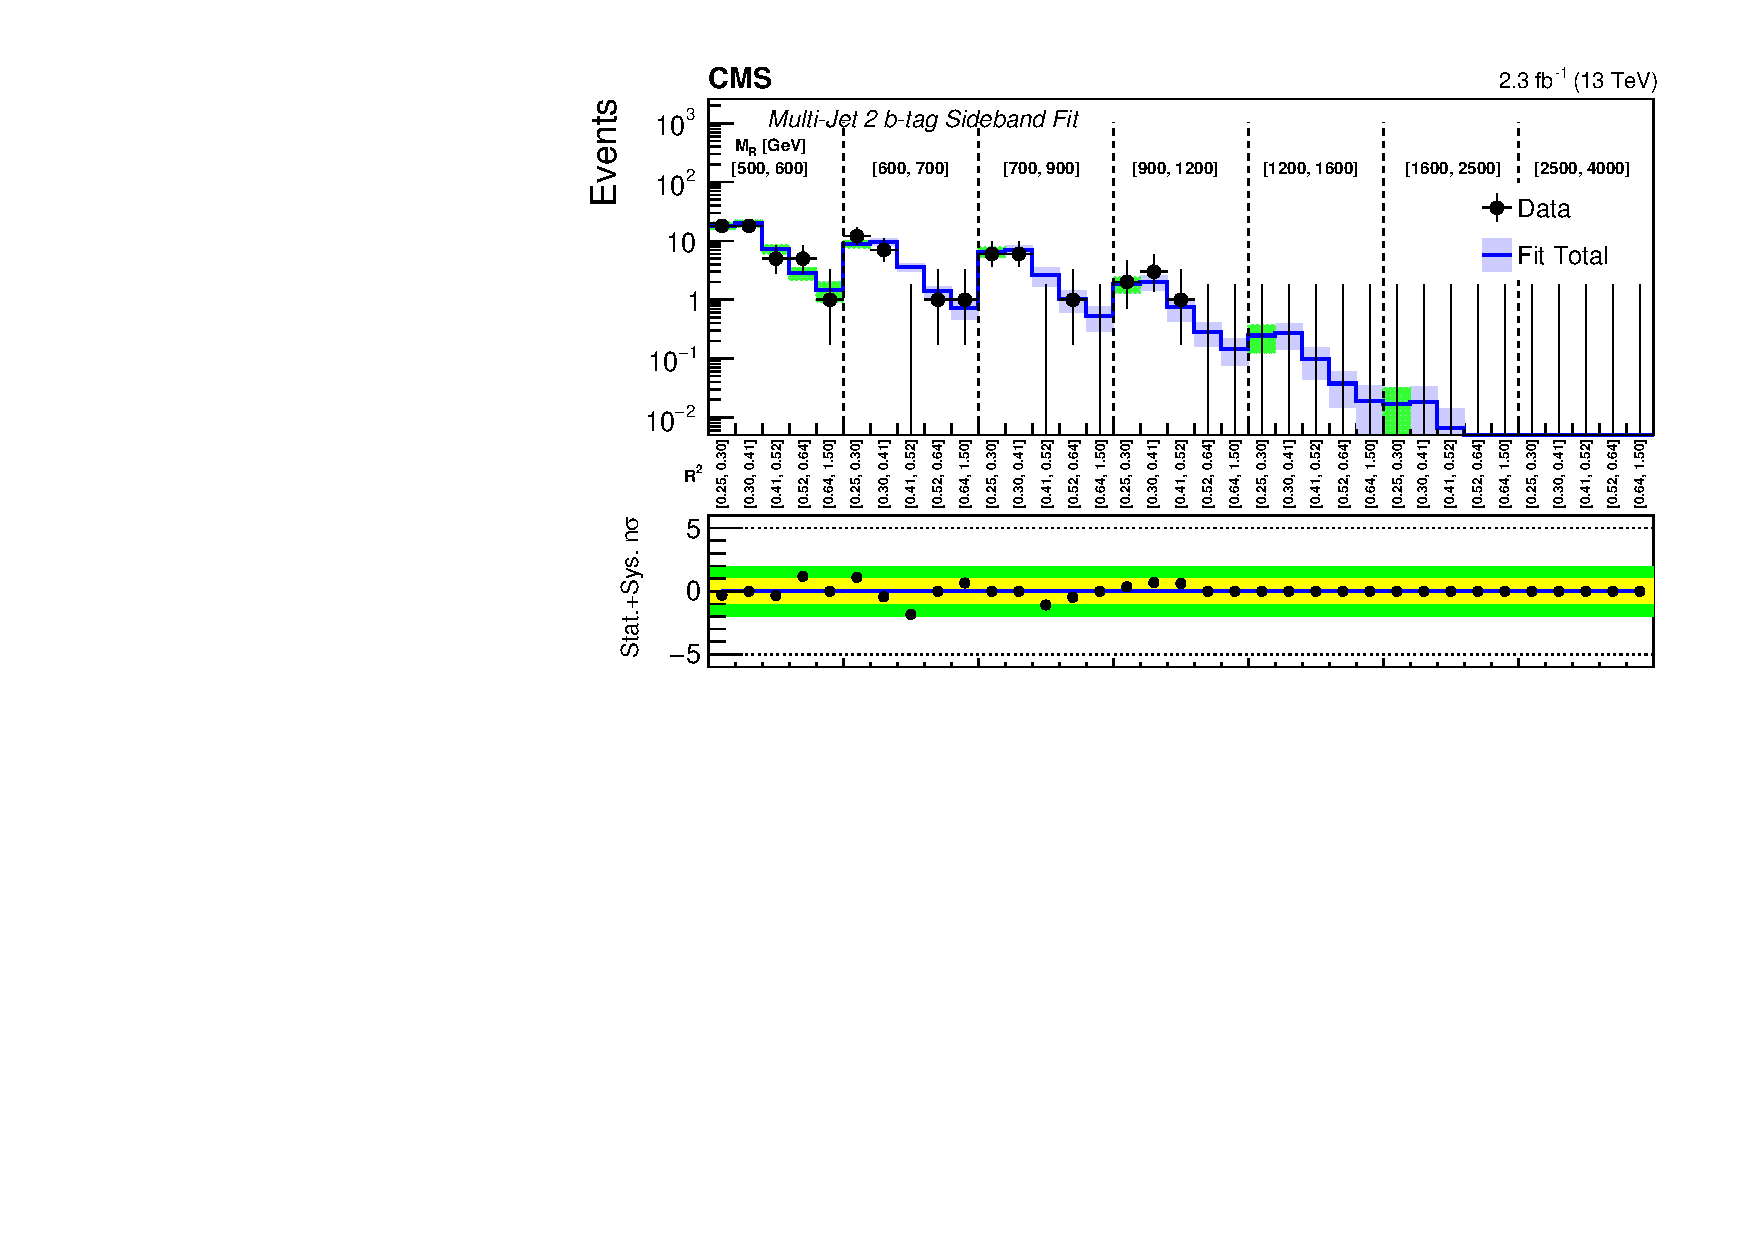
\includegraphics[width=0.9\textwidth]{figs/analysis13TeV/results/h_th1x_ns_2btag_MultiJet.pdf}}\\
\subfigure[$\geq 3$ \PQb-tag data]{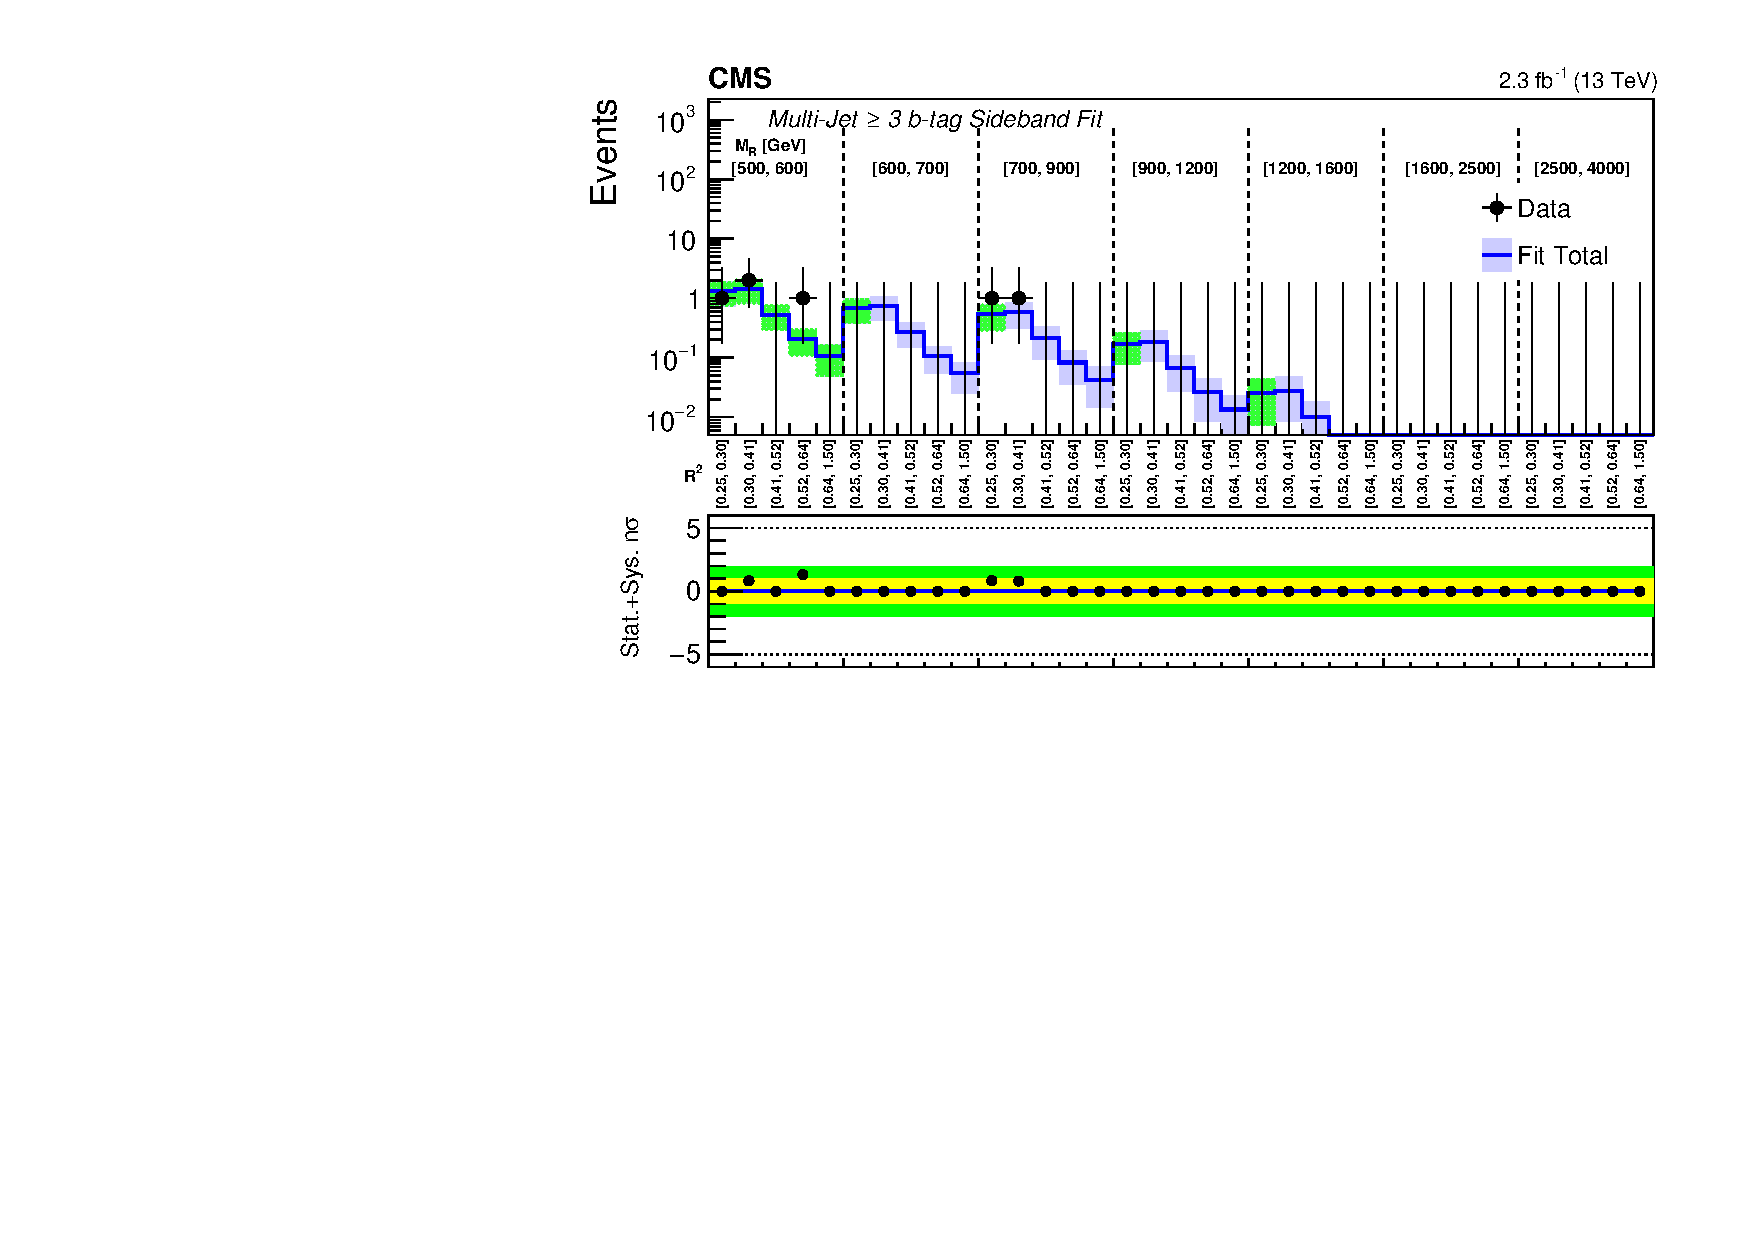
\includegraphics[width=0.9\textwidth]{figs/analysis13TeV/results/h_th1x_ns_3btag_MultiJet.pdf}}
\caption{Comparison of the sideband fit background prediction with the observed data
  in bins of $\MR$ and $\Rtwo$ variables in the Multi-Jet category for
  the 2 \PQb-tag (top) and $\geq 3$ \PQb-tag (bottom) bins. The colored bands represents the 
  systematic uncertainties in the background prediction. The uncertainty bands for the 
  sideband bins are shown in green. On the bottom inset, the deviation between the observed 
  data and the background prediction are plotted in units of standard deviation, taking into 
  account both statistical and systematic uncertainties. Vertical dashed lines denote the 
  boundaries of different $\MR$ bins. }
\label{fig:results_Multijet2btag3btag}
\end{figure}
\begin{figure}[!htb] \centering
\subfigure[2 \PQb-tag simulation]{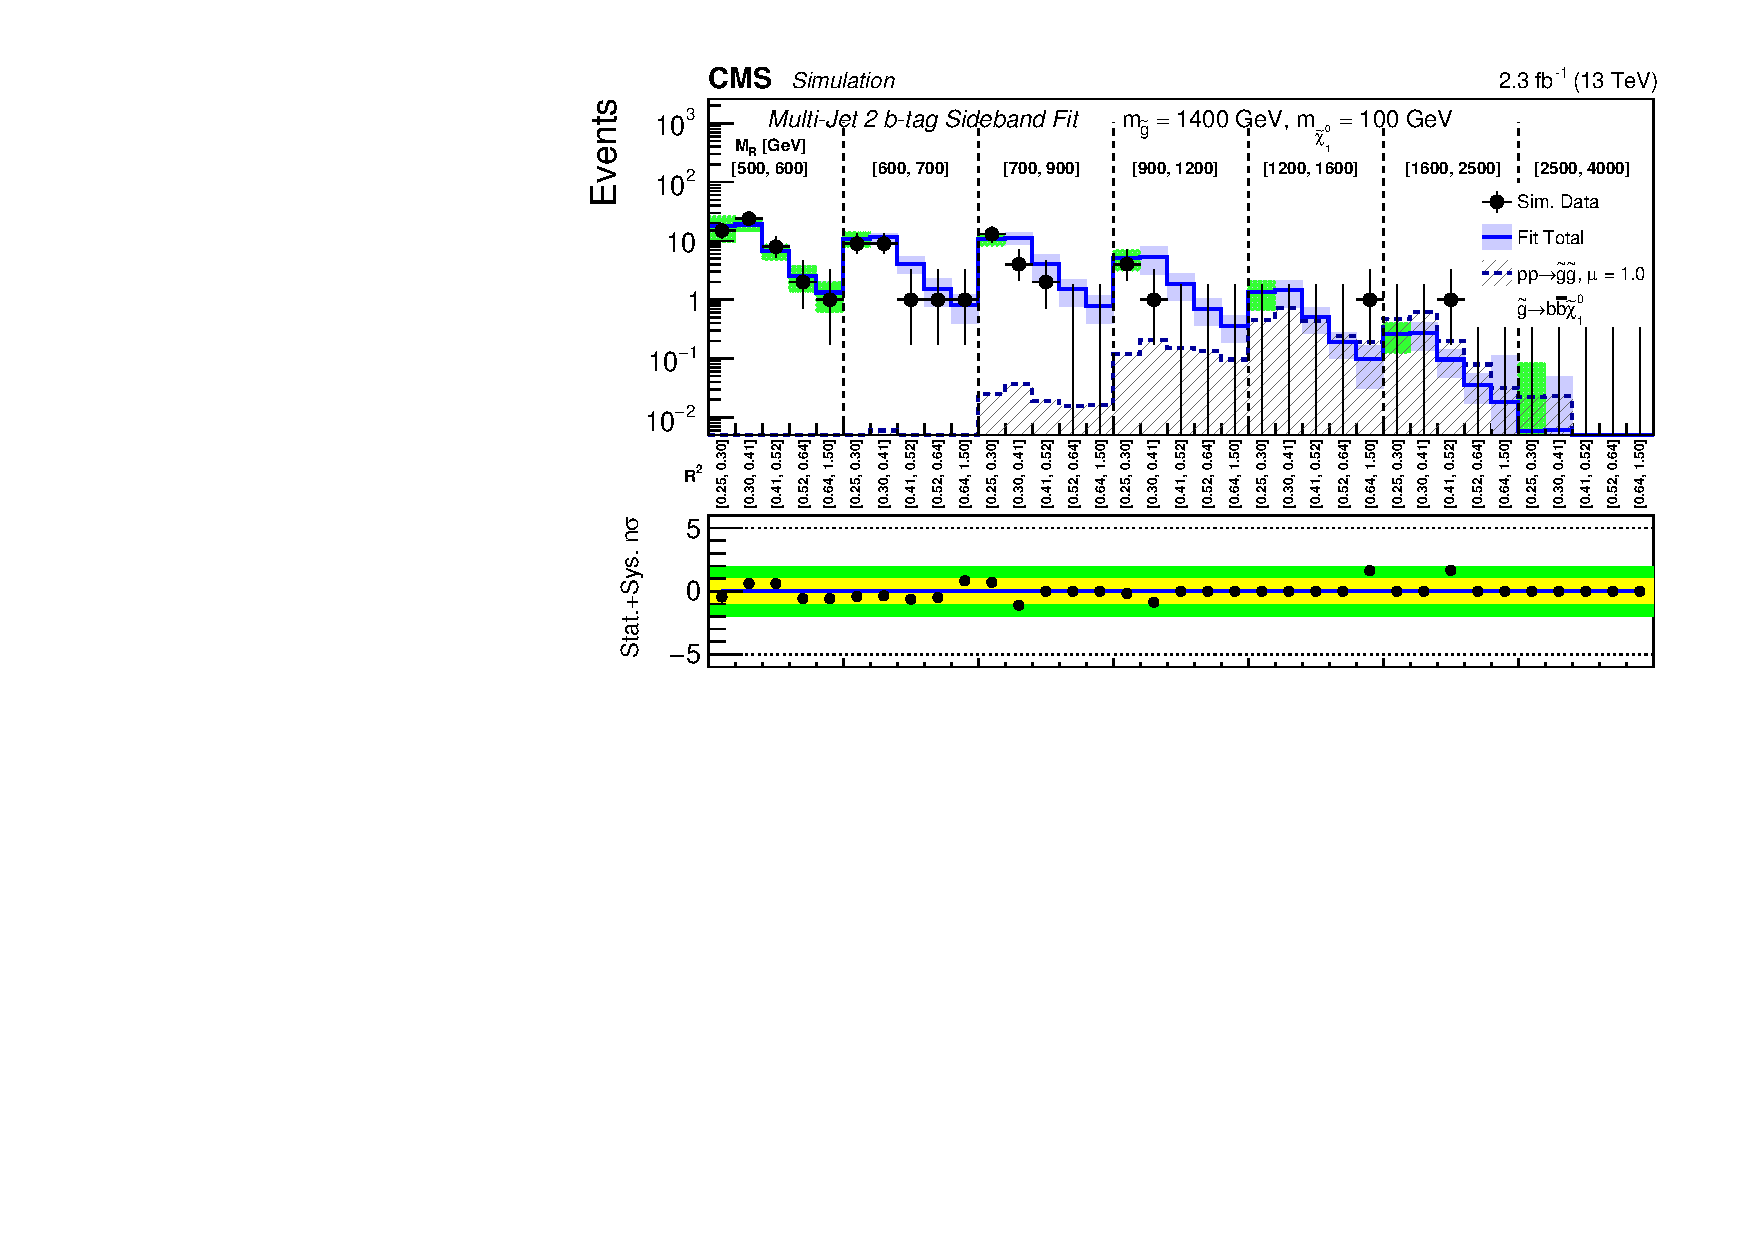
\includegraphics[width=0.9\textwidth]{figs/analysis13TeV/signalInjectionTests/T1bbbb_1400_100/h_th1x_ns_2btag_MultiJet.pdf}}\\
\subfigure[$\geq 3$ \PQb-tag simulation]{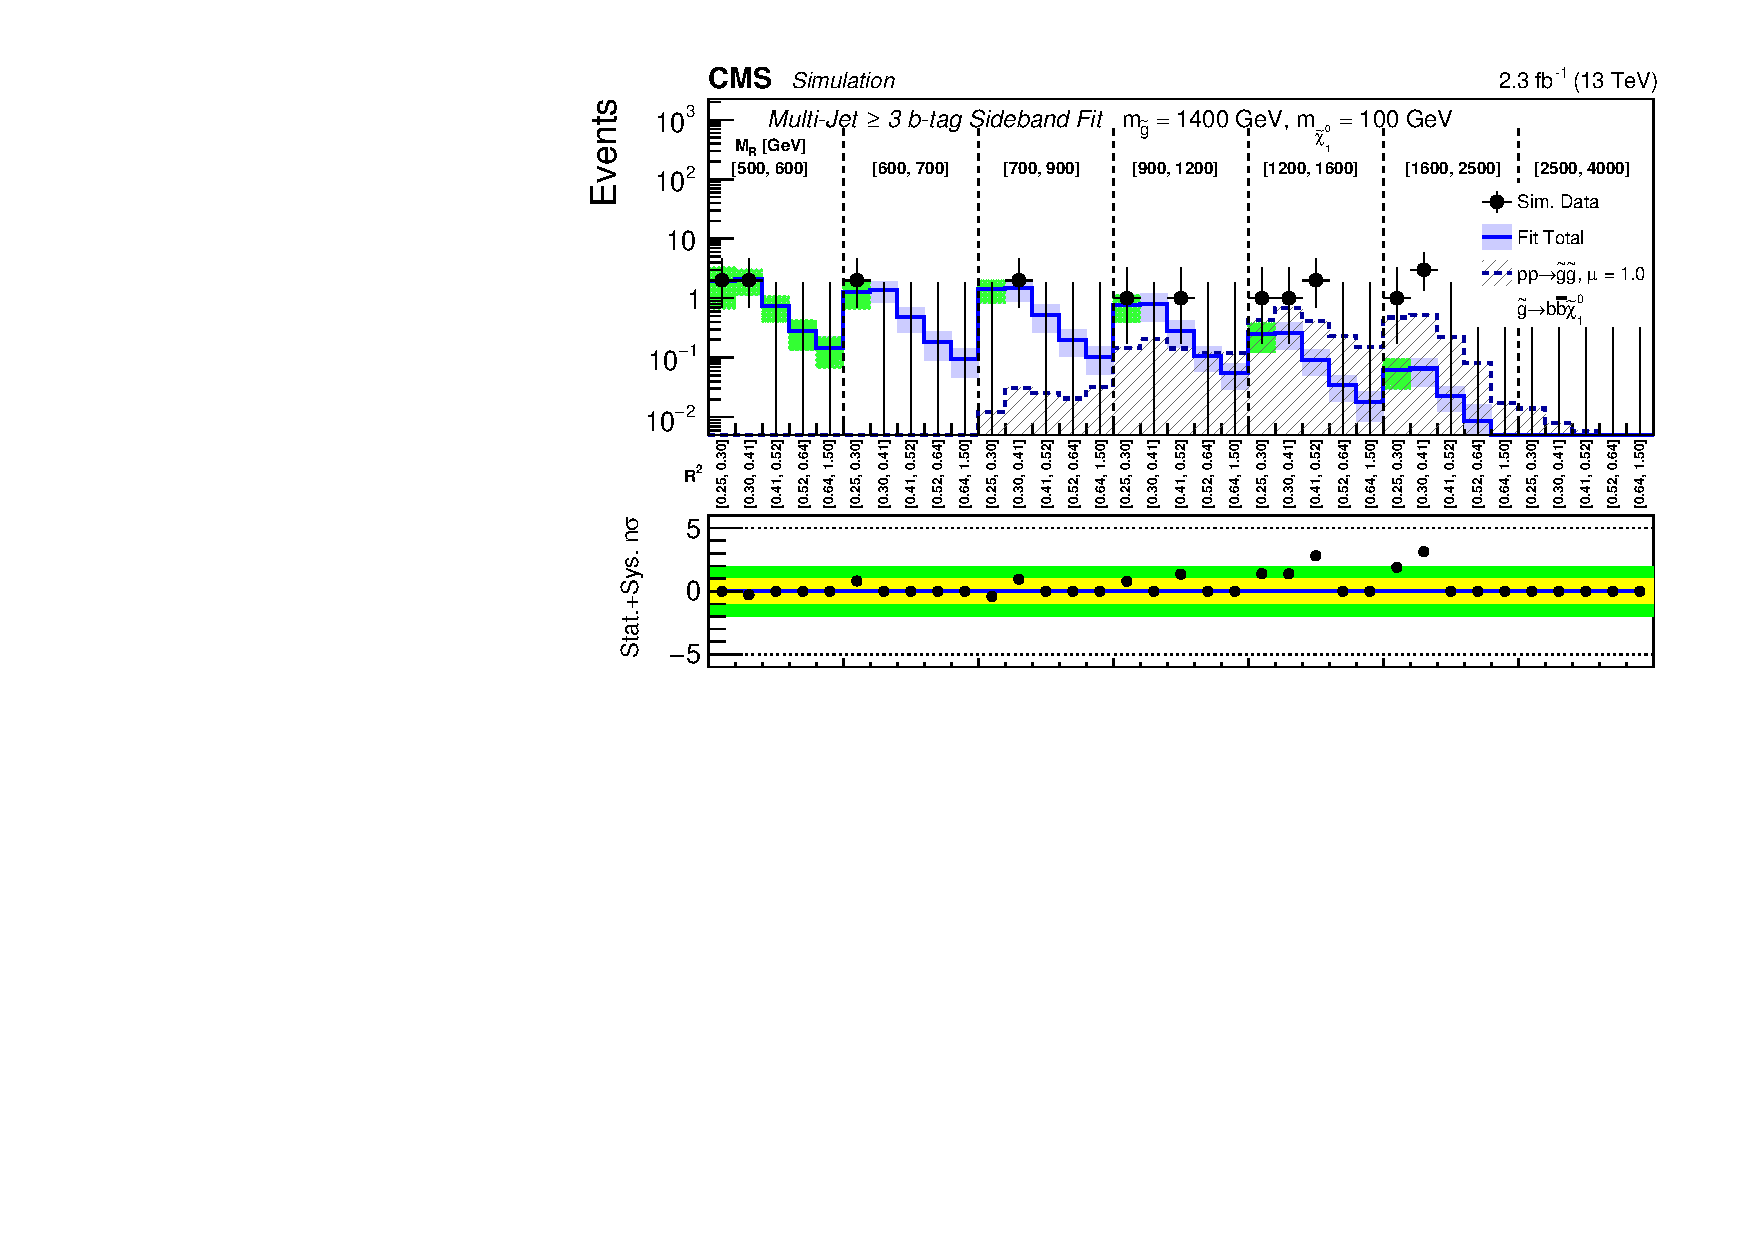
\includegraphics[width=0.9\textwidth]{figs/analysis13TeV/signalInjectionTests/T1bbbb_1400_100/h_th1x_ns_3btag_MultiJet.pdf}}
\caption{The result of the background-only fit performed in the
  sideband of the 2 \PQb-tag (top) and $\geq 3$ \PQb-tag (bottom) bins of the
  Multi-Jet category on a signal-plus-background pseudo-data set assuming a gluino pair production simplified
model signal, where gluinos decay with a 100\% branching fraction to a $\bbbar$ pair and the
 LSP, with $m_{\sGlu} = 1400 \GeV$ and  $m_{\chiz_1}=100 \GeV$, at
 nominal signal strength. A detailed explanation of the figure format is given in the caption of
  Figure~\ref{fig:results_Multijet2btag3btag}.}
\label{fig:signal_Multijet2btag3btag}
\end{figure}

To illustrate method B, we present the data and fit-based background predictions 
in Figure~\ref{fig:results_Multijet2btag3btag}, for events in the 2 \PQb-tag and $\geq 3$ \PQb-tag 
Multi-Jet categories. The number of events observed in data are compared to the
prediction from the sideband fit in the $\MR$ and $\Rtwo$ bins. To
quantify the agreement between the background model and the observation, we generate 
alternative sets of background shape parameters from the covariance matrix calculated
by the fit. An ensemble of pseudo-experiment data sets is created, generating 
random ($\MR$, $\Rtwo$) pairs distributed according to each of these alternative shapes. 
For each $\MR$-$\Rtwo$ bin, the distribution of the predicted yields from the
ensemble of pseudo-experiments is compared to the observed yield in data. 
The agreement between the predicted and the observed yields is described as a two-sided 
p-value and translated to the corresponding number of standard deviations for a normal
distribution. Positive (negative) significance indicates the observed
yield is larger (smaller) than the predicted one. We find a pattern of 
differences between the data and the background prediction in the different
bins considered that is consistent with random fluctuations.

To demonstrate that the model-independent sideband fit procedure
used in the analysis would be sensitive to the presence of a
signal, we perform a signal injection test. We sample a signal-plus-background 
pseudo-data set and perform a background-only fit in the sideband. We show one illustrative 
example of such a test in Figure~\ref{fig:signal_Multijet2btag3btag}, where we inject a signal 
corresponding to gluino pair production, in which each gluino decays to a neutralino and 
a $\bbbar$ pair with $m_{\sGlu} = 1400 \GeV$ and $m_{\chiz_1}=100 \GeV$. The
deviations with respect to the fit predictions are shown for the 2
\PQb-tag and $\geq 3$ \PQb-tag Multi-Jet categories. We observe characteristic patterns 
of excesses in two adjacent groups of bins neighboring in $\MR$. 


\subsection{Cross-Method Comparison}

The background predictions obtained from methods A and B are systematically compared 
in all of the search region categories. For method B, the model-independent 
fit to the sideband is used for this comparison. In Figure~\ref{fig:FitVsMADD},
we show the comparison of the two background predictions for two example event categories.
The predictions from the two methods agree to within the uncertainties of each method.
The uncertainty from the fit-based method tends to be slightly larger at high
$\MR$ and $\Rtwo$ due to the additional uncertainty in the exact shape of 
the tail of the distribution, as the $n$ and $b$ parameters are not strongly 
constrained by the sideband data. 

\begin{figure}[!htb] \centering
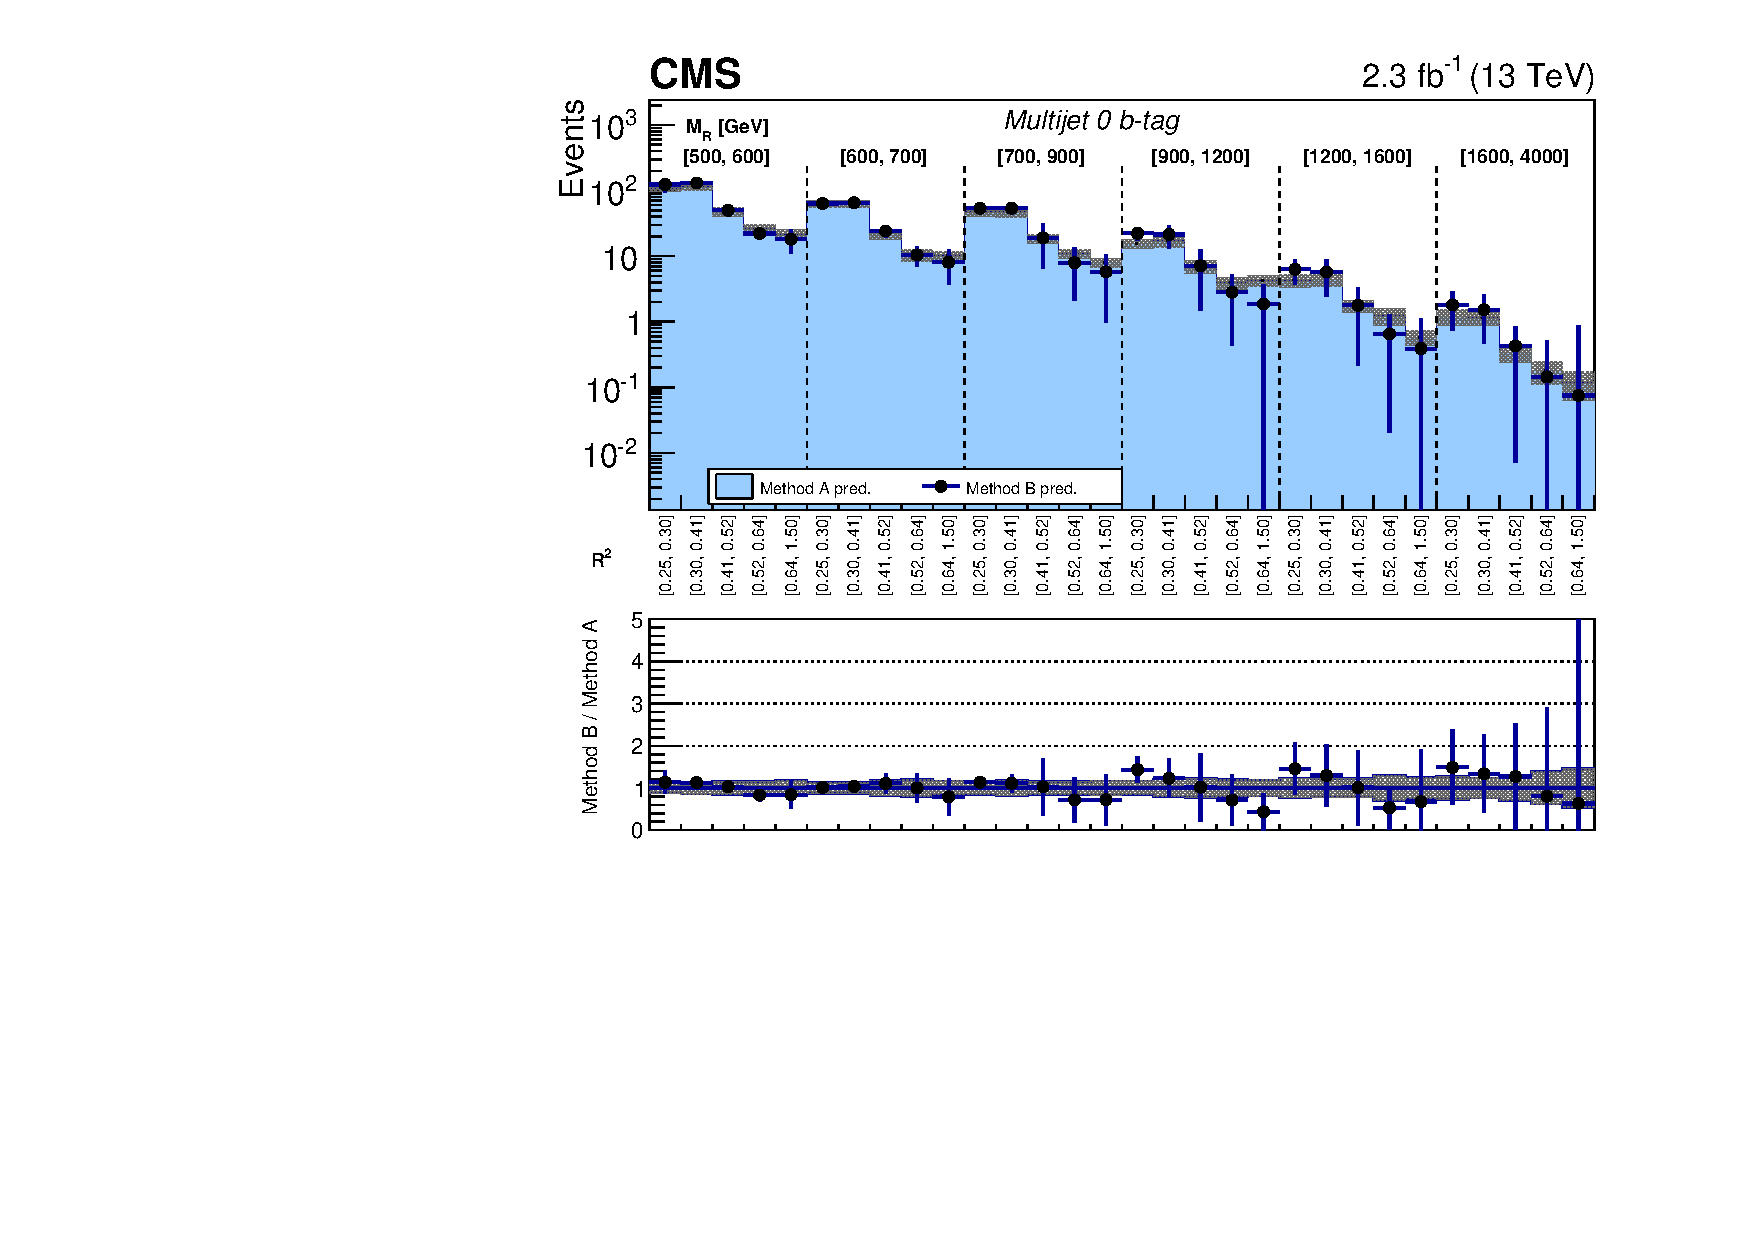
\includegraphics[width=0.9\textwidth]{figs/analysis13TeV/results/MRRsqMultiJet0BTagMCTotalUnrolledMCFit.pdf}
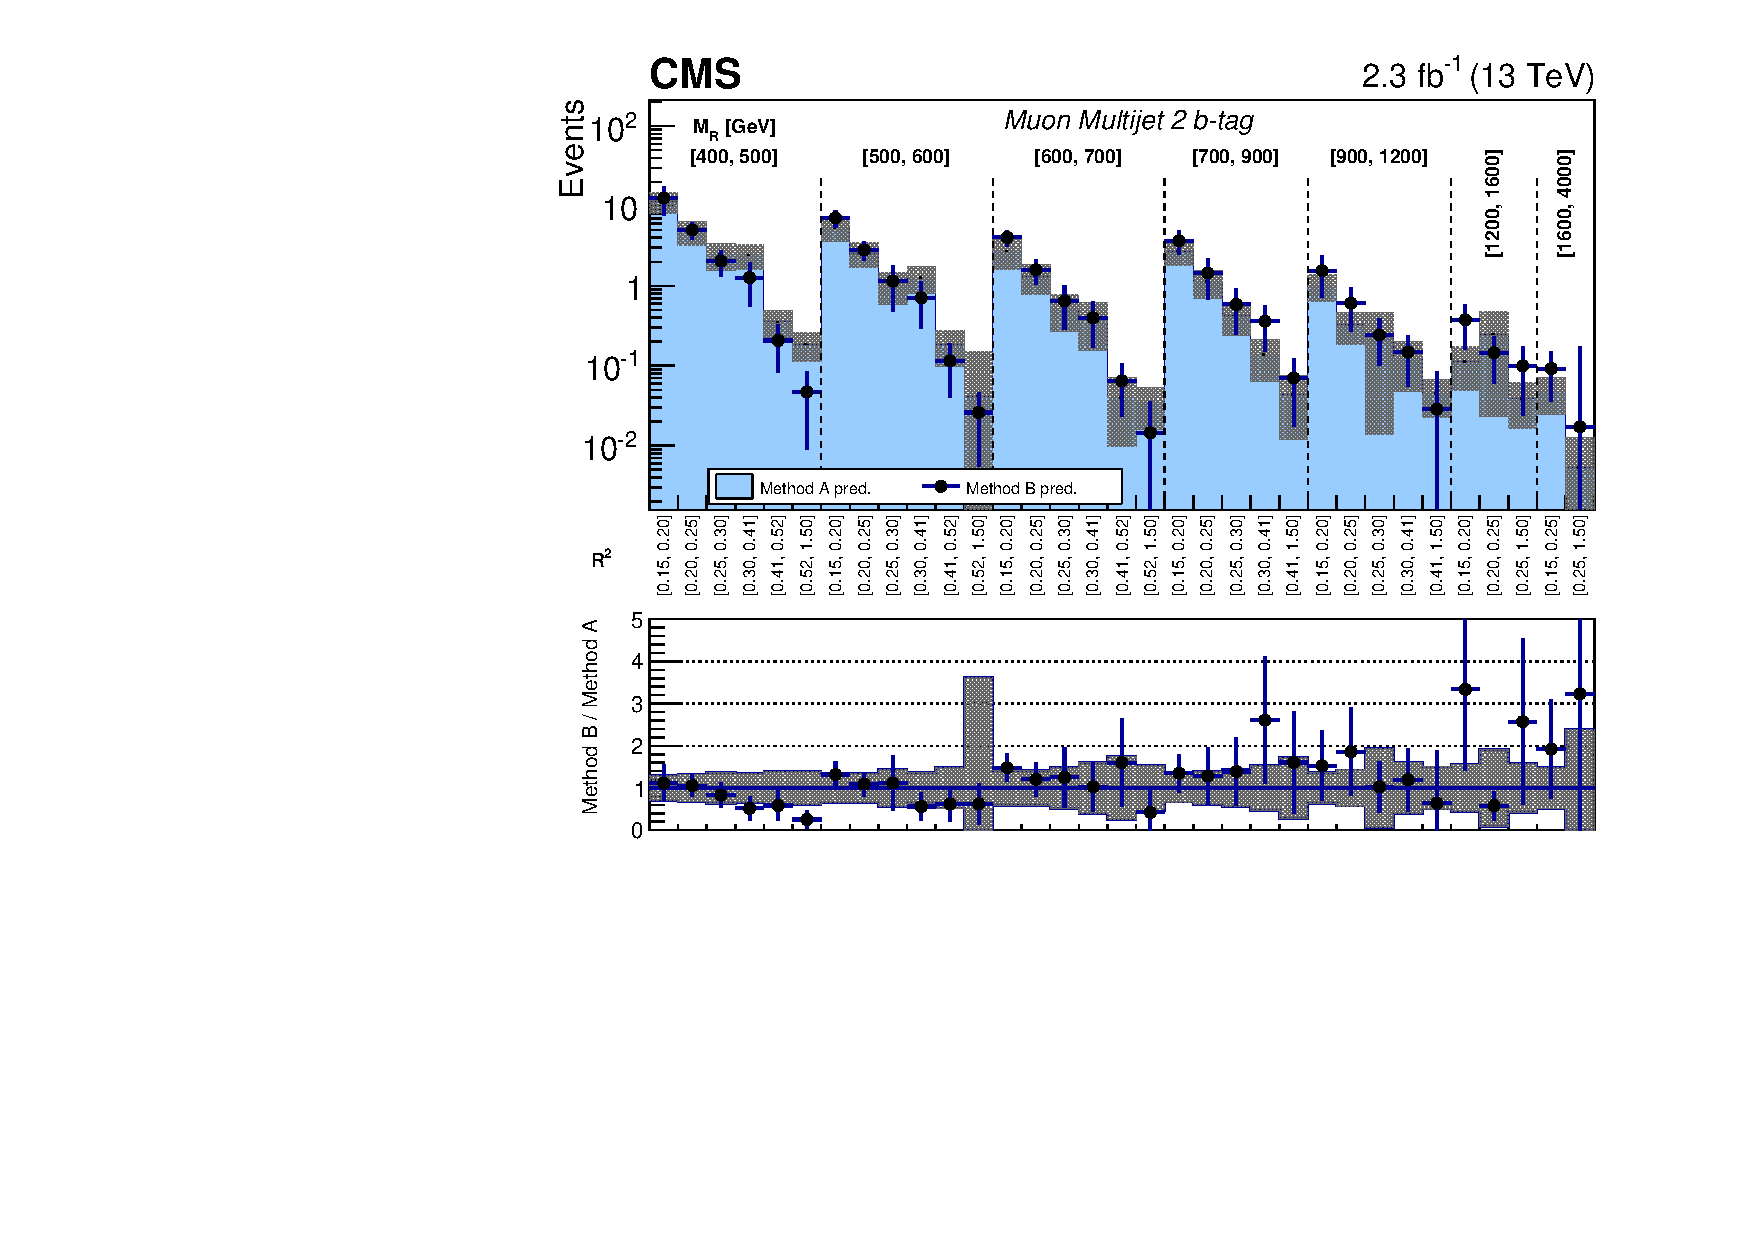
\includegraphics[width=0.9\textwidth]{figs/analysis13TeV/results/MRRsqMuMultiJet2BTagMCTotalUnrolledMCFit.pdf}
\caption{Comparisons of the two alternative background predictions for the $\MR$-$\Rtwo$ distribution 
for the 0 \PQb-tag bin of the Multi-Jet category (left) and the 2 \PQb-tag bin of the Muon Multi-Jet
category (right). The two-dimensional $\MR$-$\Rtwo$ distribution is shown
in a one dimensional representation, with each $\MR$ bin marked by the dashed lines and labeled near the top
and each $\Rtwo$ bin labeled below. The ratio of the method B prediction to the method A prediction is shown 
on the bottom inset. The method B uncertainty is represented by the error bars on the data points and the
method A uncertainty is represented by the shaded region. 
} 
\label{fig:FitVsMADD}
\end{figure}

The two background predictions use data-driven methods that make 
very different systematic assumptions. Method A assumes that corrections
to the simulation prediction measured in control regions apply also to the
signal regions, while method B assumes that the shape of the background distribution
in $\MR$ and $\Rtwo$ is well described by a particular exponentially falling functional 
form. The agreement observed between predictions obtained using these two very different 
methods significantly enhances our confidence of the background modelling, and 
also validates the respective assumptions.

\section{Systematic Uncertainties}
Various systematic uncertainties are considered in the evaluation of the
signal and background predictions. Different types of systematic
uncertainties are considered for the two different background models.

For method A, the largest uncertainties arise from the precision with
which the MC corrections are measured. The dominant uncertainties
on the correction factors result from statistical uncertainties due to 
the limited control region event sample. We also propagate systematic
uncertainties on the theoretical cross-section for the small residual backgrounds 
present in the control regions, and they contribute about $2\%$ to $5\%$ to the 
correction factor uncertainty.
Additional systematic uncertainties are computed from closure tests that 
study the accuracy of the MC corrections as a function of 
$\MR$,$\Rtwo$, and the number of \PQb-tagged jets in data events with four or more jets.
The total uncertainty from this procedure ranges from $10\%$ for the most populated bins to
$50\%$ and $100\%$ for the least populated bins. For the $\cPZ\rightarrow\nu\bar\nu$ process, we 
also propagate the difference in the correction factors measured in the three alternative 
control regions as a systematic uncertainty, intended to estimate the possible differences in 
the simulation mismodeling of the hadronic recoil for the $\cPgg$+jets process and 
the $\cPZ\rightarrow\nu\bar\nu$+jets process. These systematic uncertainties 
range from $10\%$ to $40\%$. For the QCD background prediction the statistical uncertainty 
due to limited event counts in the $\dPhiR> 2.8$ control regions and the systematic
uncertainty of $87\%$ on the translation factor $\zeta$ are propagated.
Finally, the contribution of potential SUSY signal events in the control regions are
propagated as a systematic uncertainty on the background estimate 
and is seen to have a very limited effect on the interpretation of the result.

For method B, the systematic uncertainties on the background are propagated as part of 
the maximum likelihood fit procedure. For each event category, the background shape in 
$\MR$ and $\Rtwo$ is described by four independent parameters: two 
that control the exponential fall off and two that control the behavior of the
non-exponential tail. Systematic uncertainties on the background are propagated 
through the profiling of these unconstrained shape parameters. For more populated bins, such as 
the 0 \PQb-tag and 1 \PQb-tag bins in the MultiJet category, the systematic uncertainties range from
about 30\% at low $\MR$ and $\Rtwo$ to about 70\% at high $\MR$ and $\Rtwo$.
For sparsely populated bins such as the 3 or more \PQb-tag bin in the Muon MultiJet or Electron
MultiJet categories, the systematic uncertainties range from
about 60\% at low $\MR$ and $\Rtwo$ to more than 200\% at high $\MR$ and $\Rtwo$.

\begin{table}[!htb]
\begin{center}
\caption{Summary of the main instrumental and theoretical systematic uncertainties.}
\label{tab:BackgroundSystematics}
\resizebox{\textwidth}{!}{
\begin{tabular}{|c|c|c|}
\hline
Systematic Uncertainty Source      & On Signal and/or Bkg   & Typical Impact of Uncertainty on Yields \\
\hline
Jet Energy Scale                   & Both                   & $2-15\%$ \\ \hline
Electron Energy Scale              & Both                   & $7-9\%$ \\ \hline
Muon Momentum Scale                & Both                   & $7-9\%$ \\ \hline
Muon efficiency                    & Both                   & $7-8\%$ \\ \hline
Electron efficiency                & Both                   & $7-8\%$ \\ \hline
Trigger efficiency                 & Both                   & $3\%$ \\ \hline
\PQb-tagging  efficiency           & Both                   & $6-15\%$ \\ \hline
\PQb mistagging  efficiency        & Both                   & $4-7\%$ \\ \hline
Ren./Fac.\ Scale                   & Both                   & $10-25\%$ \\\hline
Luminosity                         & Both                   & $2.7\%$ \\\hline
%Pileup                            & Both                   & $1\%$ \\ \hline
%Monte Carlo Statistics            & Both                   & $1/\sqrt{N_{MC}}$ \\\hline
Fast Simulation corrections        & Signal Only            & $0-10\%$ \\ \hline
Initial State Radiation            & Signal Only            & $15 - 30\%$ only for recoil above $400$~GeV \\\hline
\end{tabular}}
\end{center}
\end{table}

Systematic uncertainties due to instrumental and theoretical effects are propagated as shape 
uncertainties on the signal predictions for method A and B, and on the background
predictions for method A. The background prediction from method B is not affected
by these uncertainties as the shape and normalization are measured from data.
Uncertainties on the trigger and lepton selection efficiency, and the 
integrated luminosity primarily affect the total normalization. Uncertainties in 
the b-tagging efficiency affect the relative yields between different b-tag categories. 
The uncertainties from missing higher order corrections and the uncertainties on the jet 
energy and lepton momentum scale affect the shapes of the $\MR$ and $\Rtwo$ distributions.

For the signal predictions, we also propagate systematic uncertainties due to
possible inaccuracies of the fast simulation in modeling the lepton selection and 
b-tagging efficiencies. Finally, we propagate an uncertainty on the modeling of initial 
state radiation for signal predictions, that ranges from $15\%$ for signal events with 
recoil between $400\GeV$ and $600\GeV$ to $30\%$ for events with recoil above $600\GeV$. 
The systematic uncertainties and their typical impact on background and signal
predictions are summarized in Table~\ref{tab:BackgroundSystematics}.



\section{Results and Interpretations}
\label{sec:Results}

We present results of the search using method A as it provides slightly better sensitivity.
The two-dimensional $\MR$-$\Rtwo$ distributions for the search regions in the 
Multi-Jet, Electron Multi-Jet, and Muon Multi-Jet categories observed in data are shown in 
Figures~\ref{fig:ResultsMultiJet0btag1btag},\ref{fig:ResultsMultiJet2btag3btag},~\ref{fig:ResultsMuMultiJet0btag1btag},~\ref{fig:ResultsMuMultiJet2btag3btag},~\ref{fig:ResultsEleMultiJet0btag1btag},~and~\ref{fig:ResultsEleMultiJet2btag3btag},
along with the background prediction from method A. 
We observed no statistically significant discrepancies and interpret the null search
result using method A in terms of limits on the production cross section for the SUSY 
simplified model scenarios discussed in Section~\ref{sec:intro}.

\begin{figure}[!htb] \centering
\subfigure[0 \PQb-tag data]{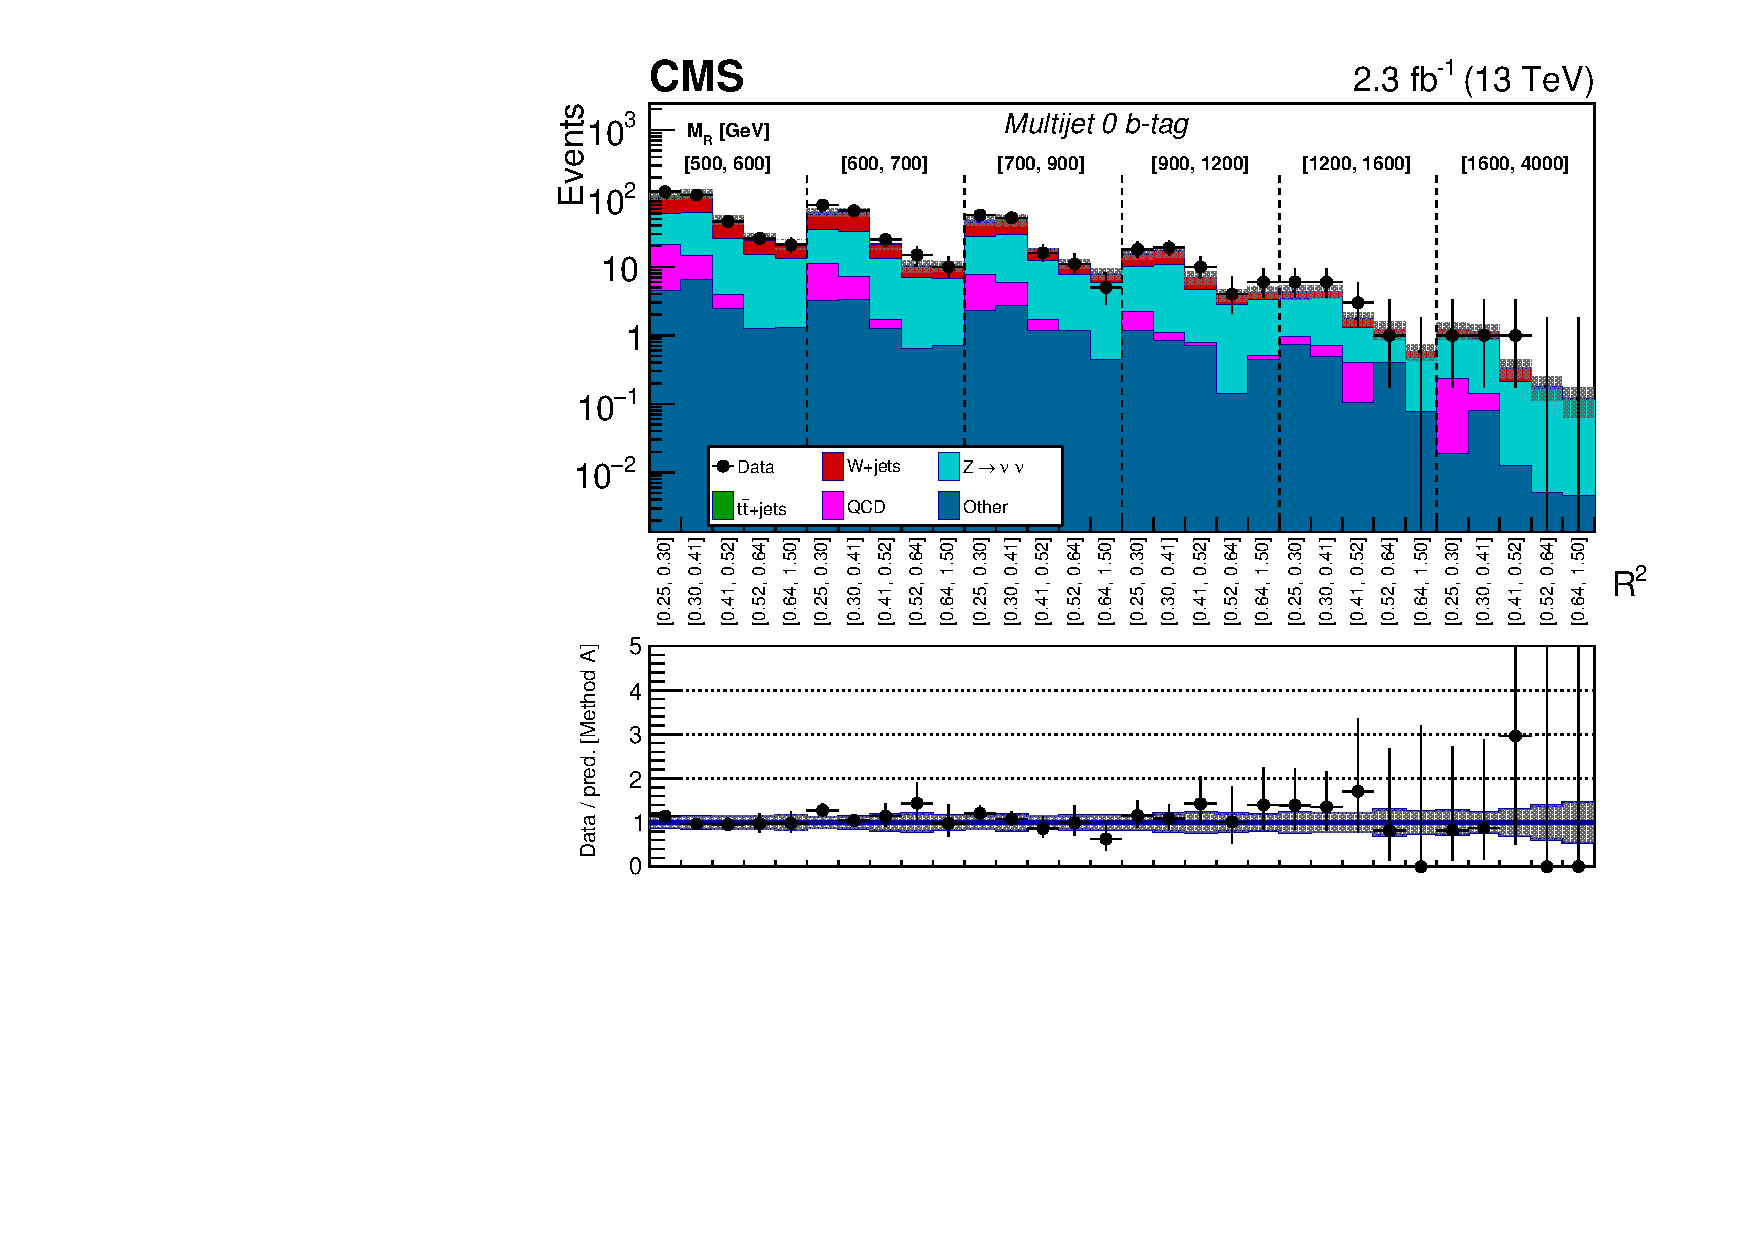
\includegraphics[width=0.8\textwidth]{figs/analysis13TeV/results/MRRsqMultiJet0BTagUnrolledDataMC.pdf}}\\
\subfigure[1 \PQb-tag data]{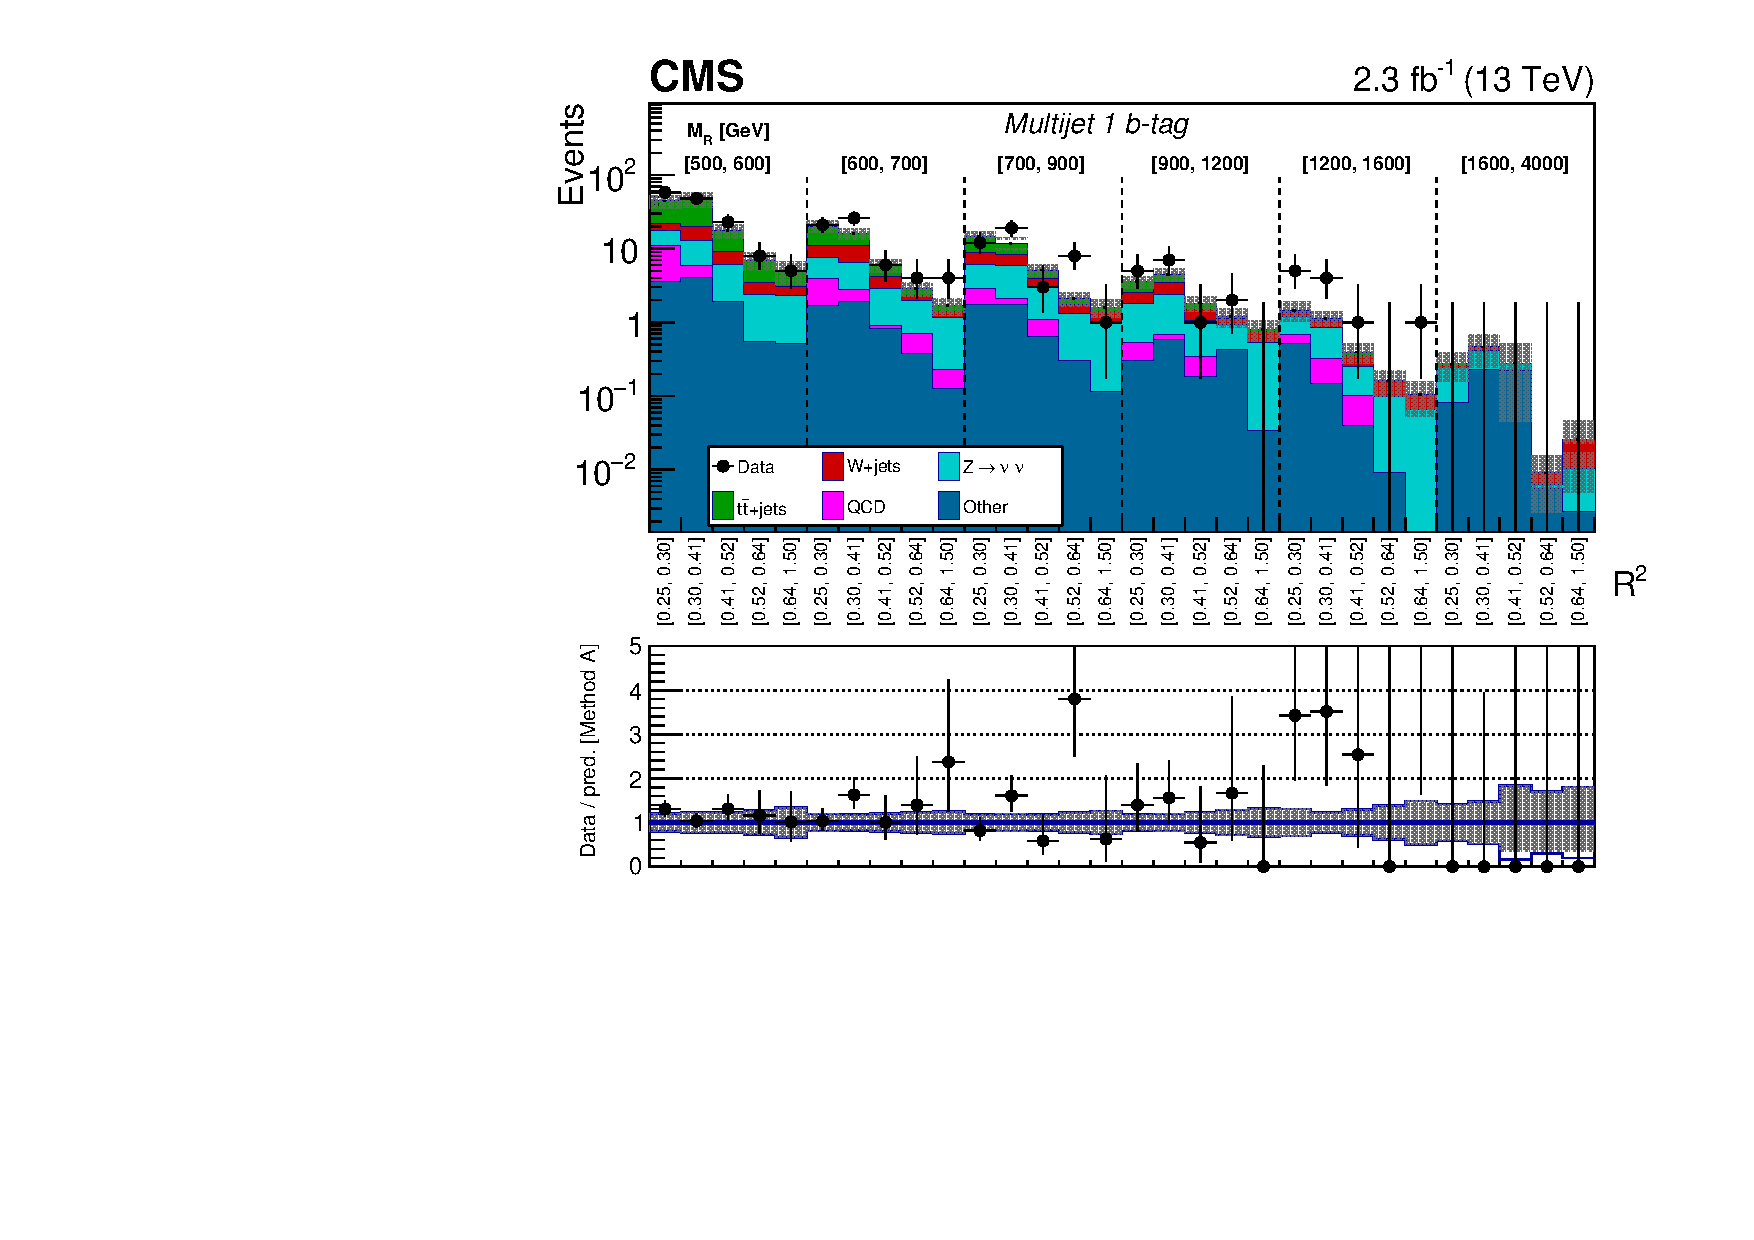
\includegraphics[width=0.8\textwidth]{figs/analysis13TeV/results/MRRsqMultiJet1BTagUnrolledDataMC.pdf}}
\caption{ The $\MR$-$\Rtwo$ distribution observed in data is shown along with the background prediction
obtained from method A for the Multi-Jet event category in the 0
\PQb-tag (top) and 1 \PQb-tag (bottom) bins. The two-dimensional $\MR$-$\Rtwo$ distribution is shown
in a one dimensional representation, with each $\MR$ bin marked by the dashed lines and labeled near the top,
and each $\Rtwo$ bin labeled below. The ratio of data to the background prediction is shown on the bottom inset, with
the statistical uncertainty expressed through the data point error bars and the systematic uncertainty of the
background prediction represented by the shaded region. 
}
\label{fig:ResultsMultiJet0btag1btag}
\end{figure}

\begin{figure}[!htb] \centering
\subfigure[2 \PQb-tag data]{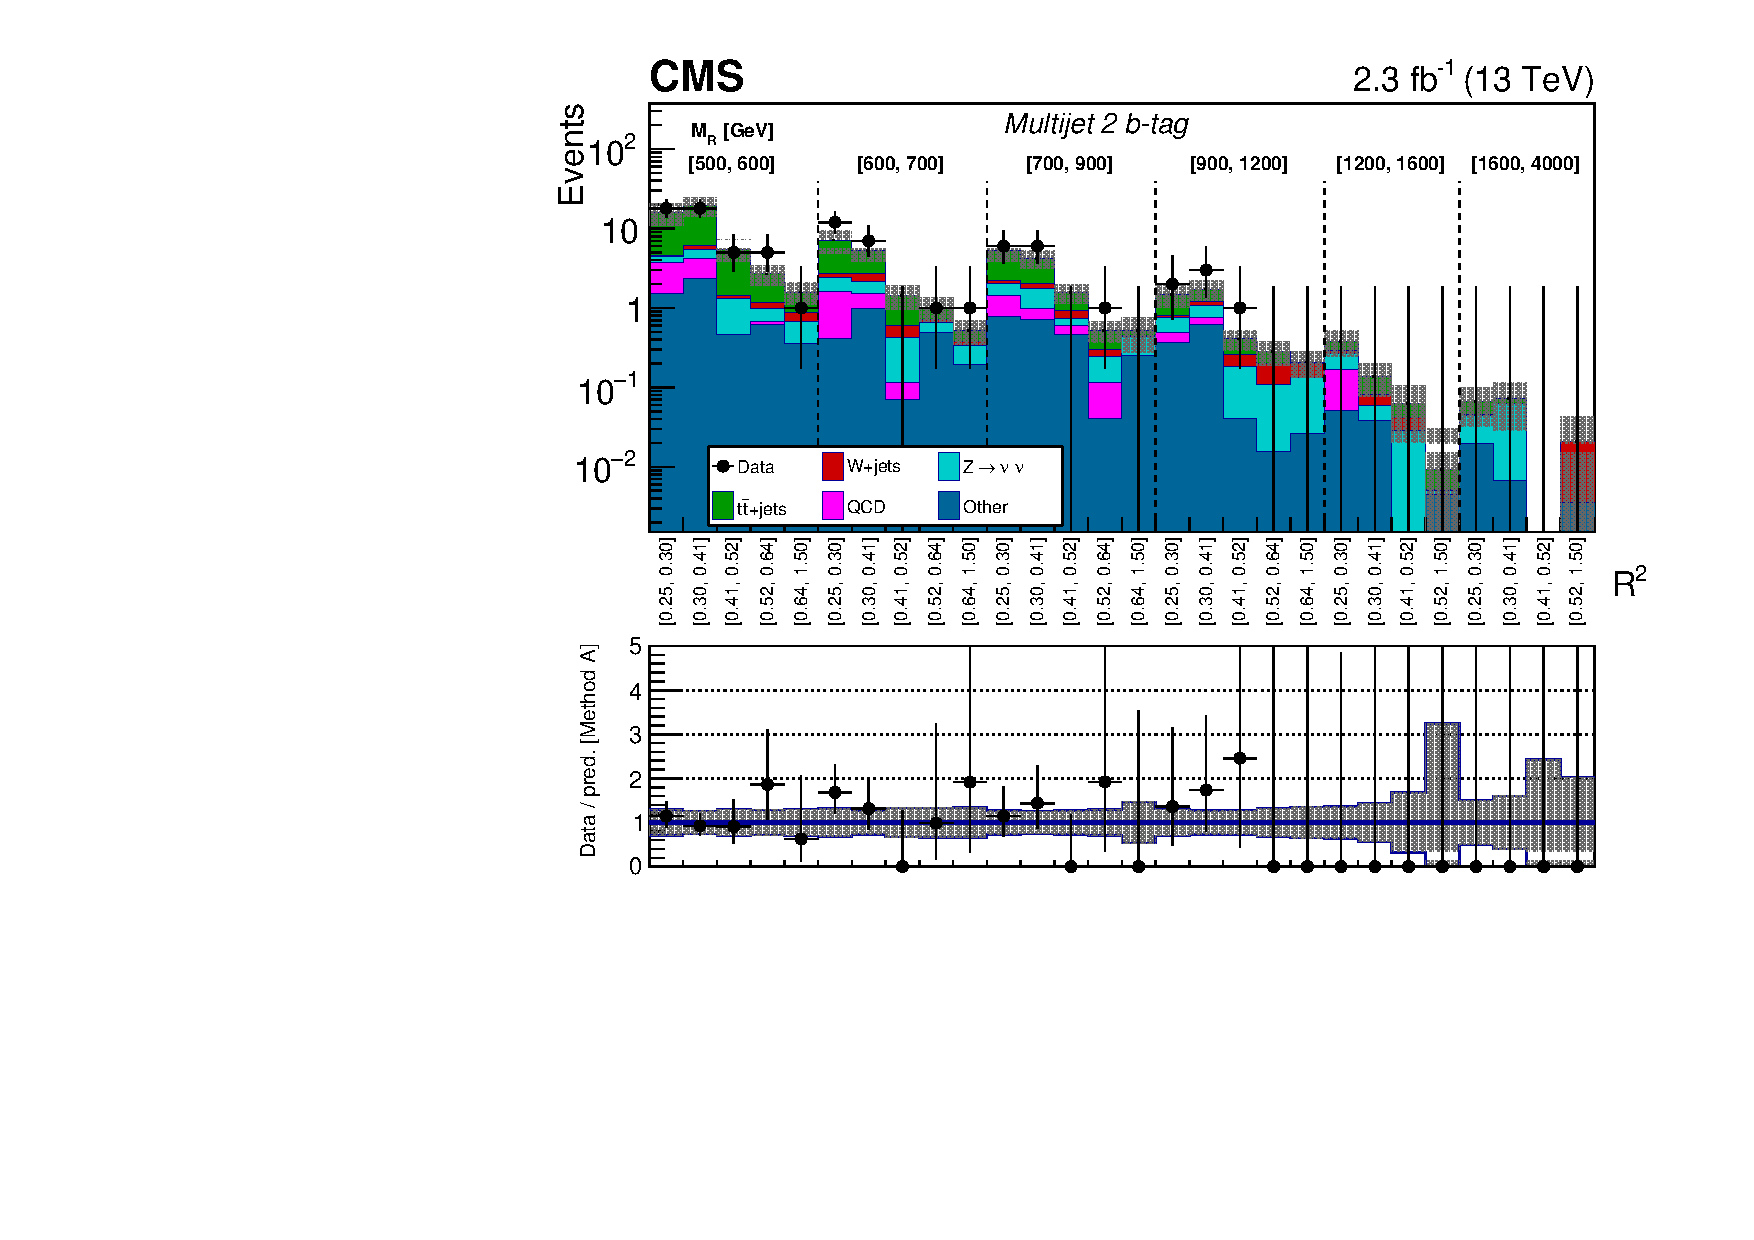
\includegraphics[width=0.8\textwidth]{figs/analysis13TeV/results/MRRsqMultiJet2BTagUnrolledDataMC.pdf}}\\
\subfigure[$\geq$ 3 \PQb-tag data]{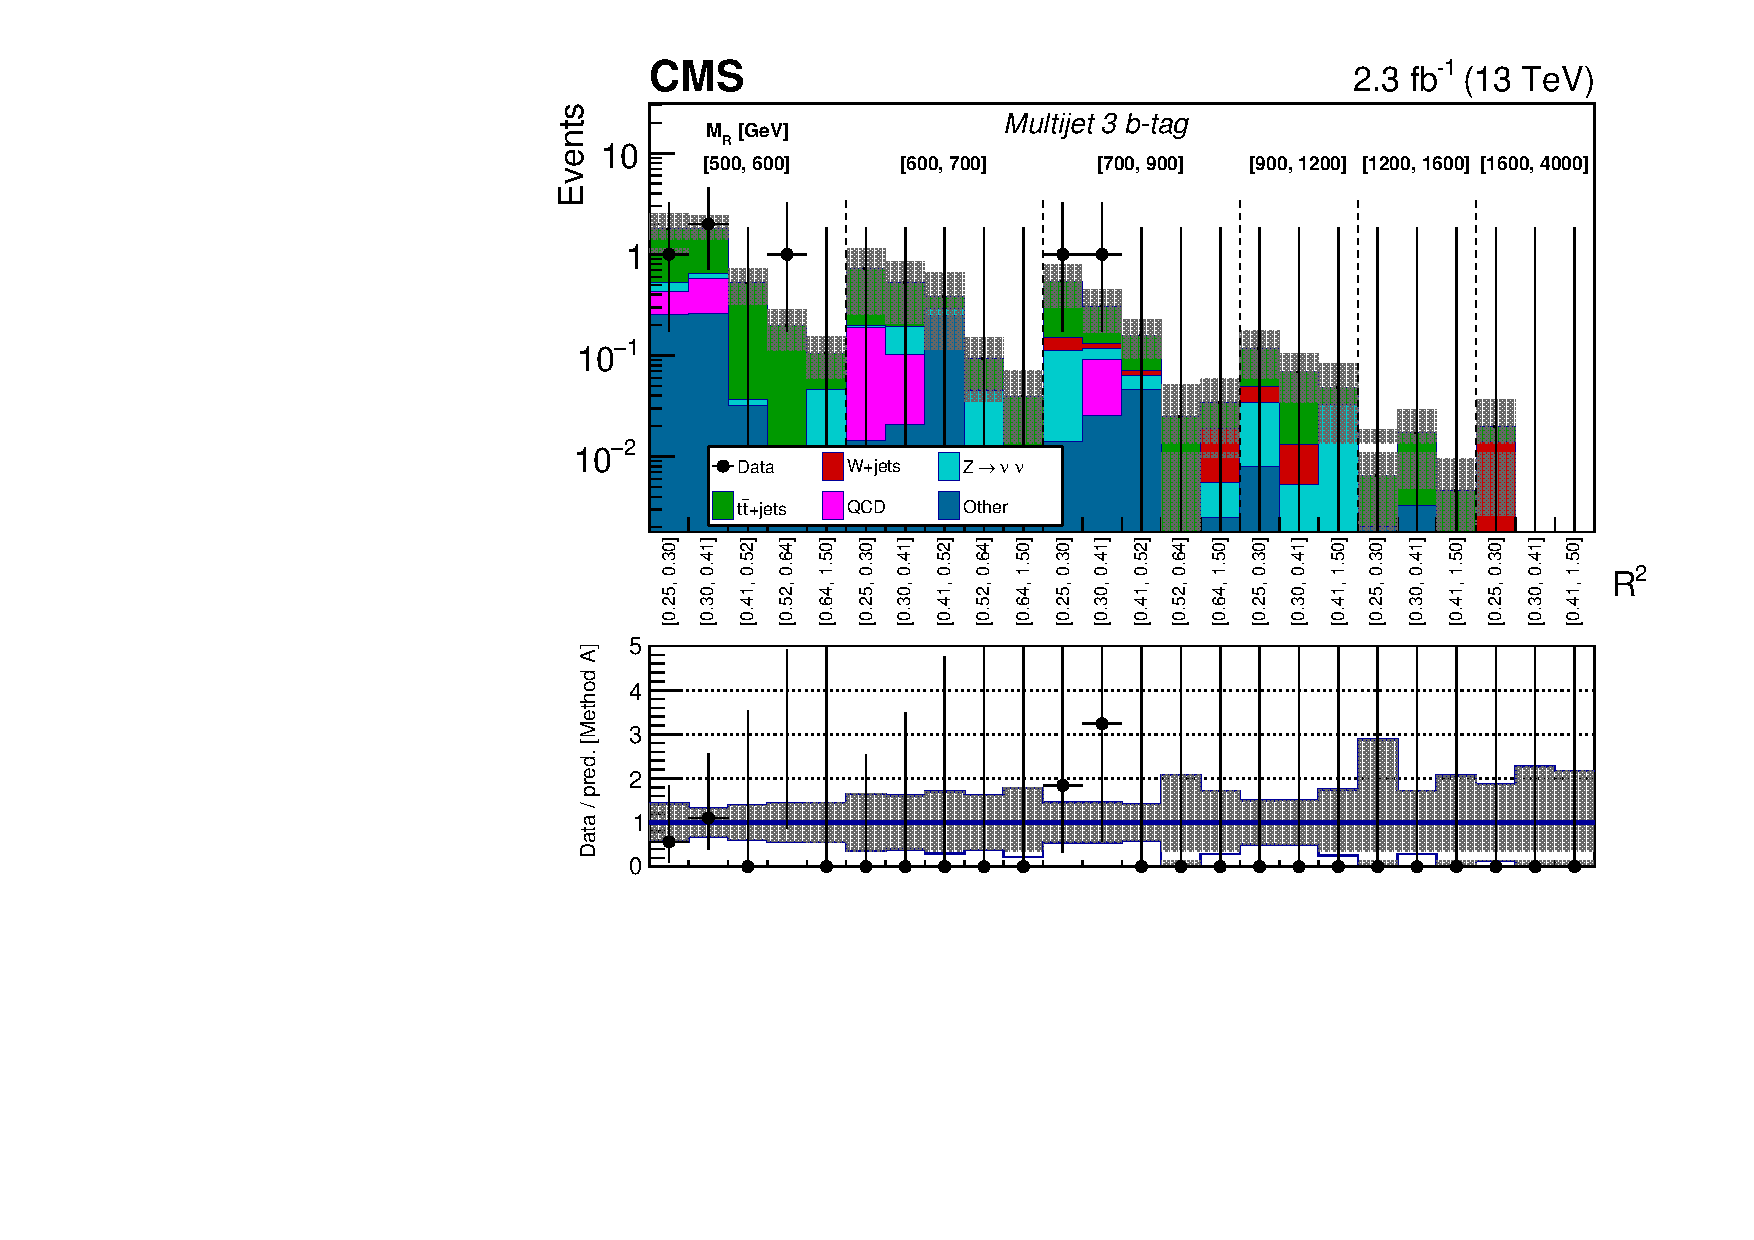
\includegraphics[width=0.8\textwidth]{figs/analysis13TeV/results/MRRsqMultiJet3BTagUnrolledDataMC.pdf}}
\caption{ The $\MR$-$\Rtwo$ distribution observed in data is shown along with the background prediction
obtained from method A for the Multi-Jet event category in the 2 \PQb-tag (top) and $\geq 3$ \PQb-tag (bottom) bins. 
A detailed explanation of the plots is given in the caption of
  Figure~\ref{fig:ResultsMultiJet0btag1btag}.
}
\label{fig:ResultsMultiJet2btag3btag}
\end{figure}

\begin{figure}[!htb] \centering
\subfigure[0 \PQb-tag data]{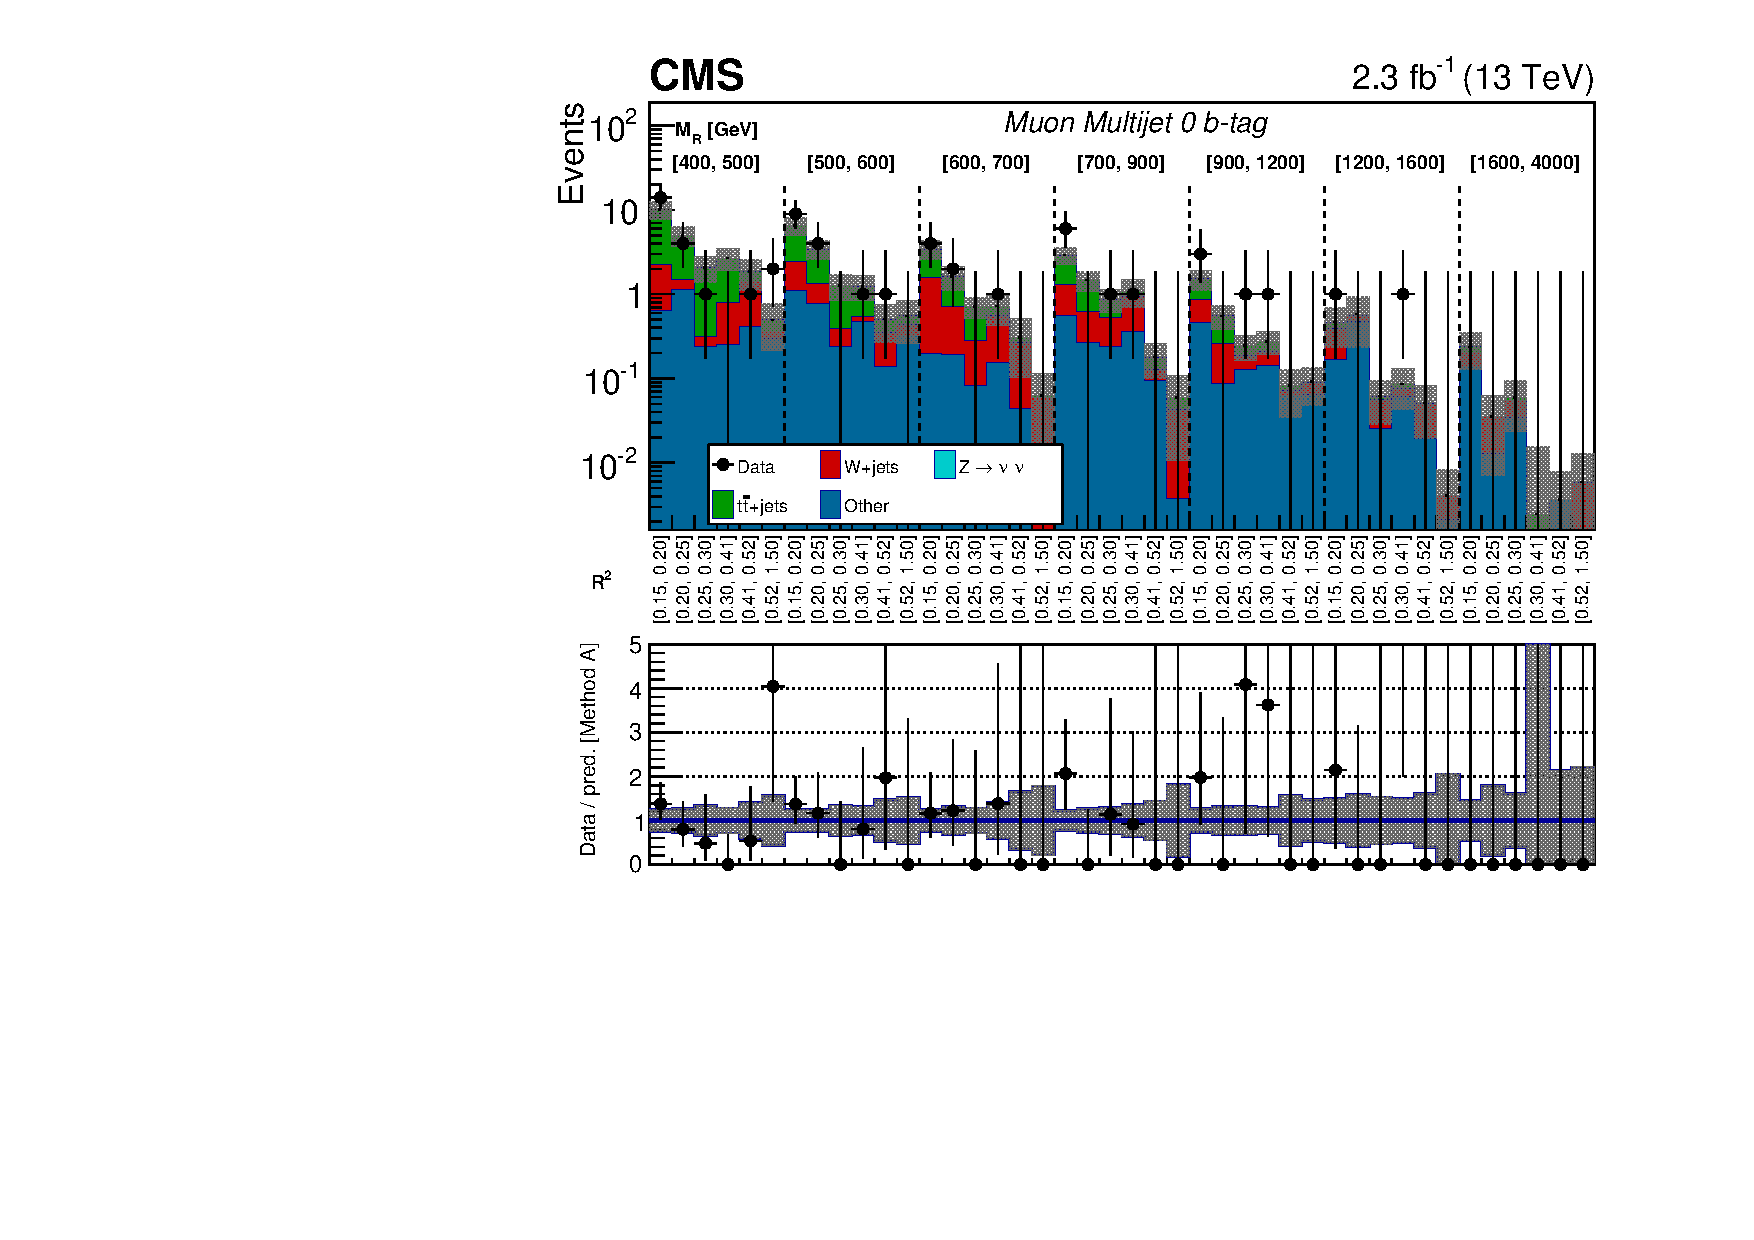
\includegraphics[width=0.8\textwidth]{figs/analysis13TeV/results/MRRsqMuMultiJet0BTagUnrolledDataMC.pdf}}\\
\subfigure[1 \PQb-tag data]{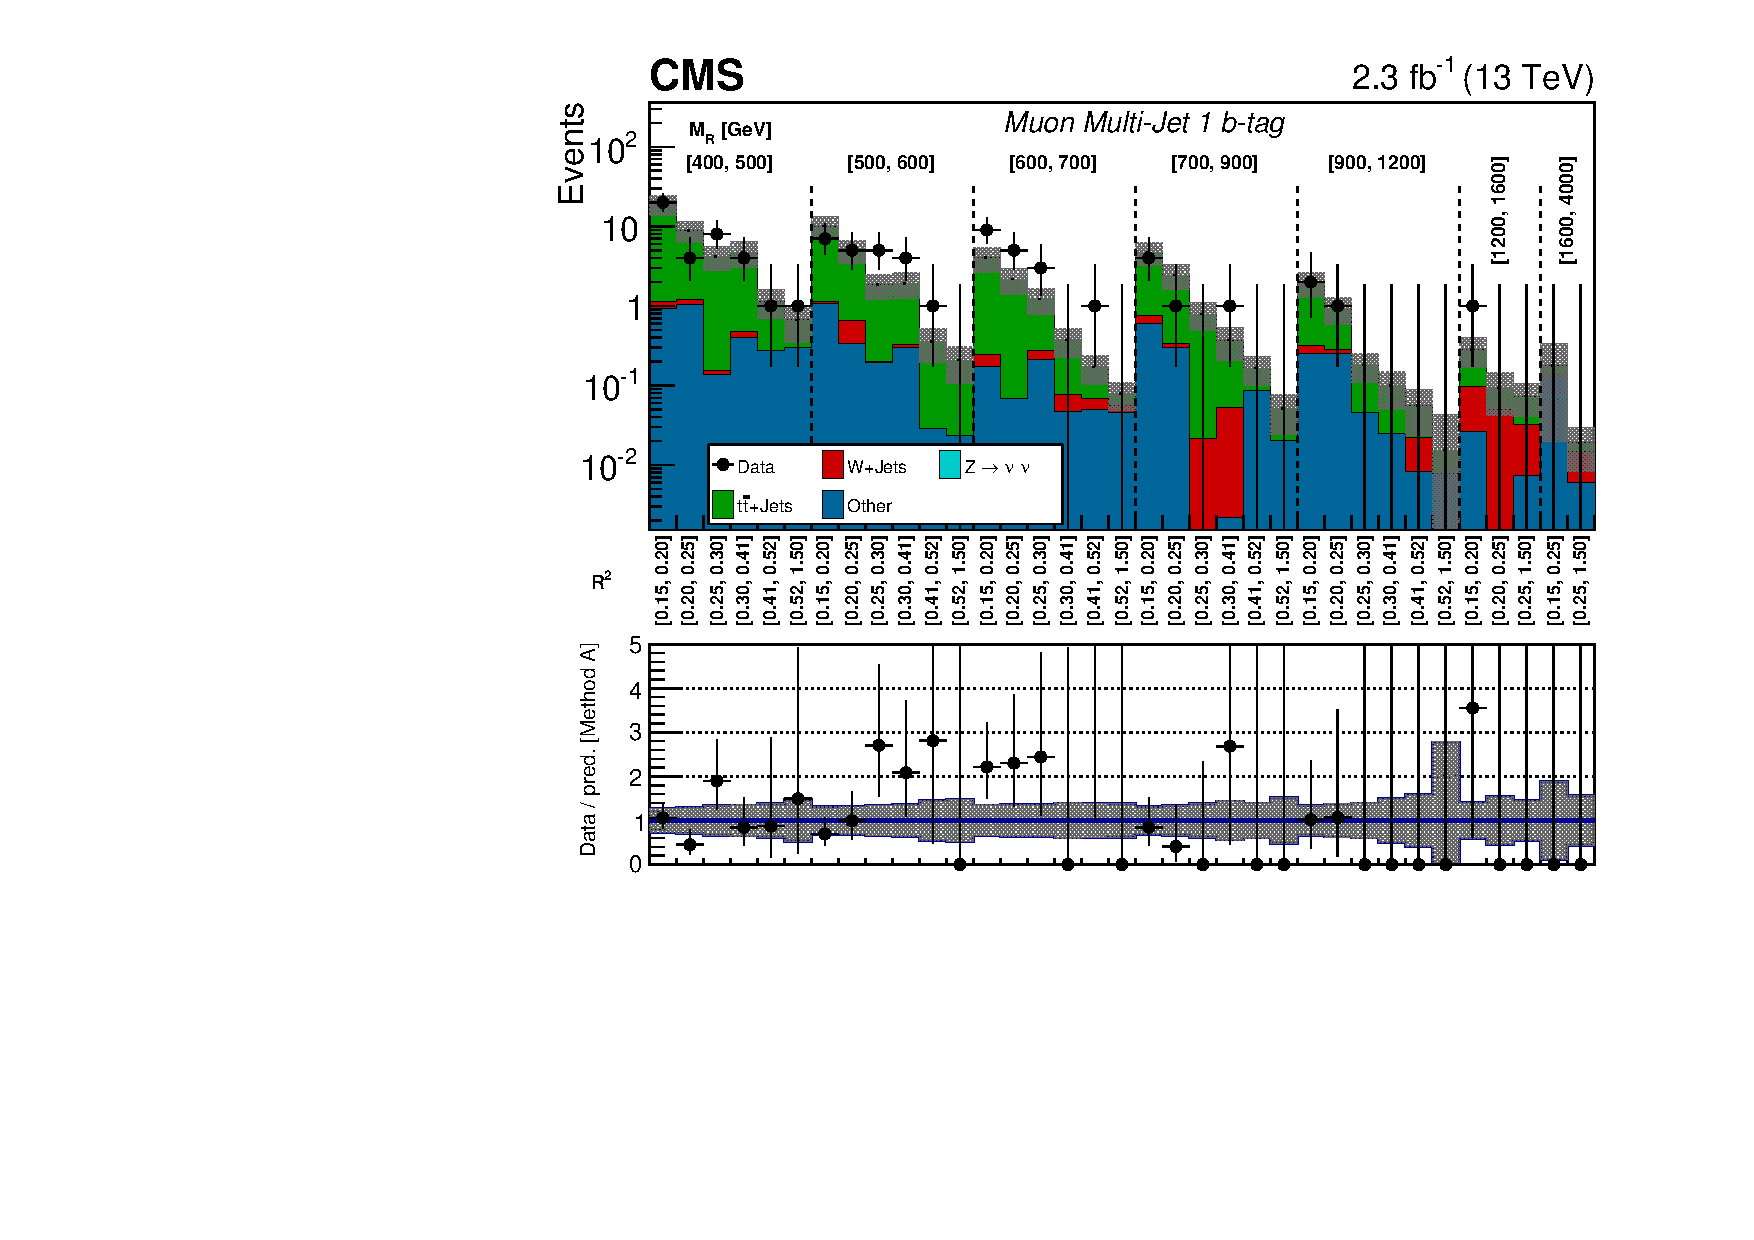
\includegraphics[width=0.8\textwidth]{figs/analysis13TeV/results/MRRsqMuMultiJet1BTagUnrolledDataMC.pdf}}
\caption{ The $\MR$-$\Rtwo$ distribution observed in data is shown along with the background prediction
obtained from method A for the Muon Multi-Jet event category in the 0 \PQb-tag (top) and 1 \PQb-tag (bottom) bins. 
A detailed explanation of the plots is given in the caption of
  Figure~\ref{fig:ResultsMultiJet0btag1btag}.
}
\label{fig:ResultsMuMultiJet0btag1btag}
\end{figure}

\begin{figure}[!htb] \centering
\subfigure[2 \PQb-tag data]{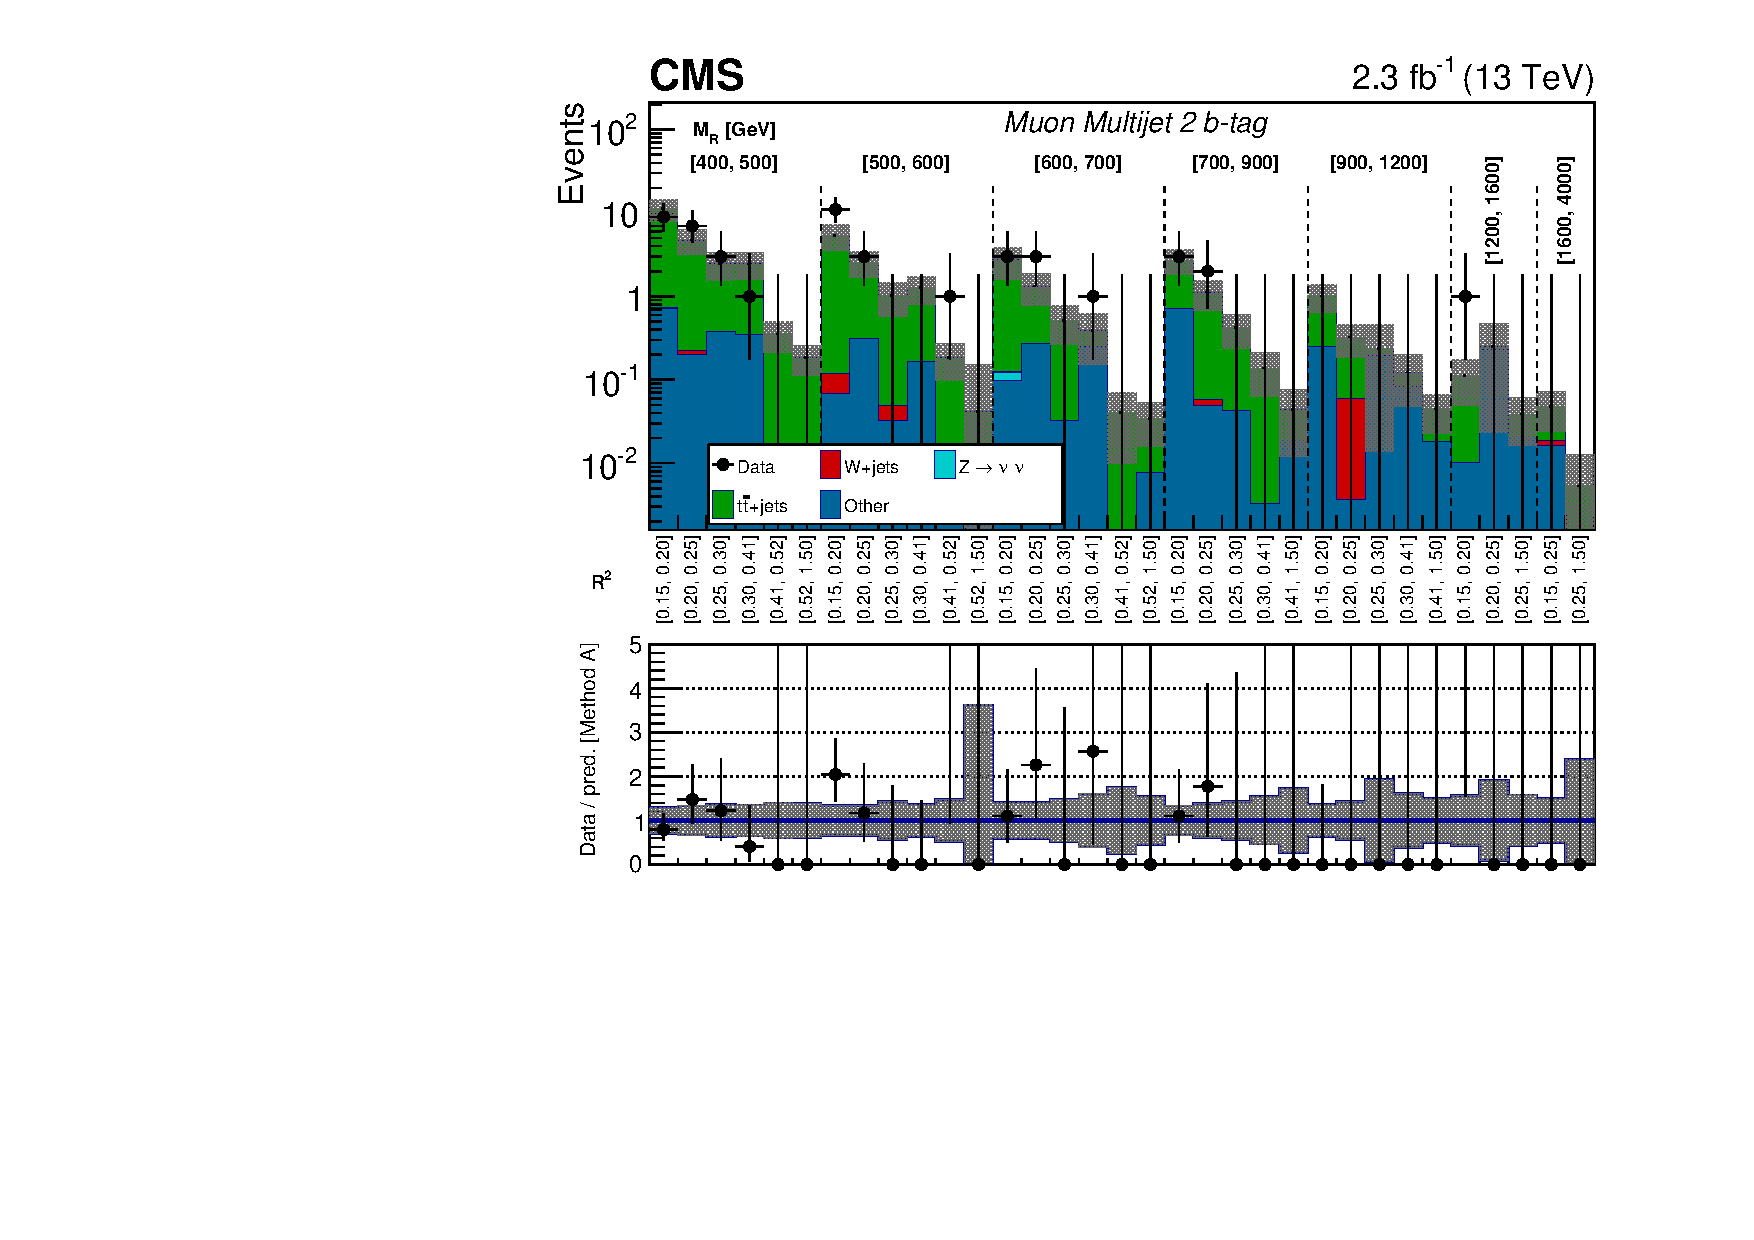
\includegraphics[width=0.8\textwidth]{figs/analysis13TeV/results/MRRsqMuMultiJet2BTagUnrolledDataMC.pdf}}\\
\subfigure[$\geq$ 3 \PQb-tag data]{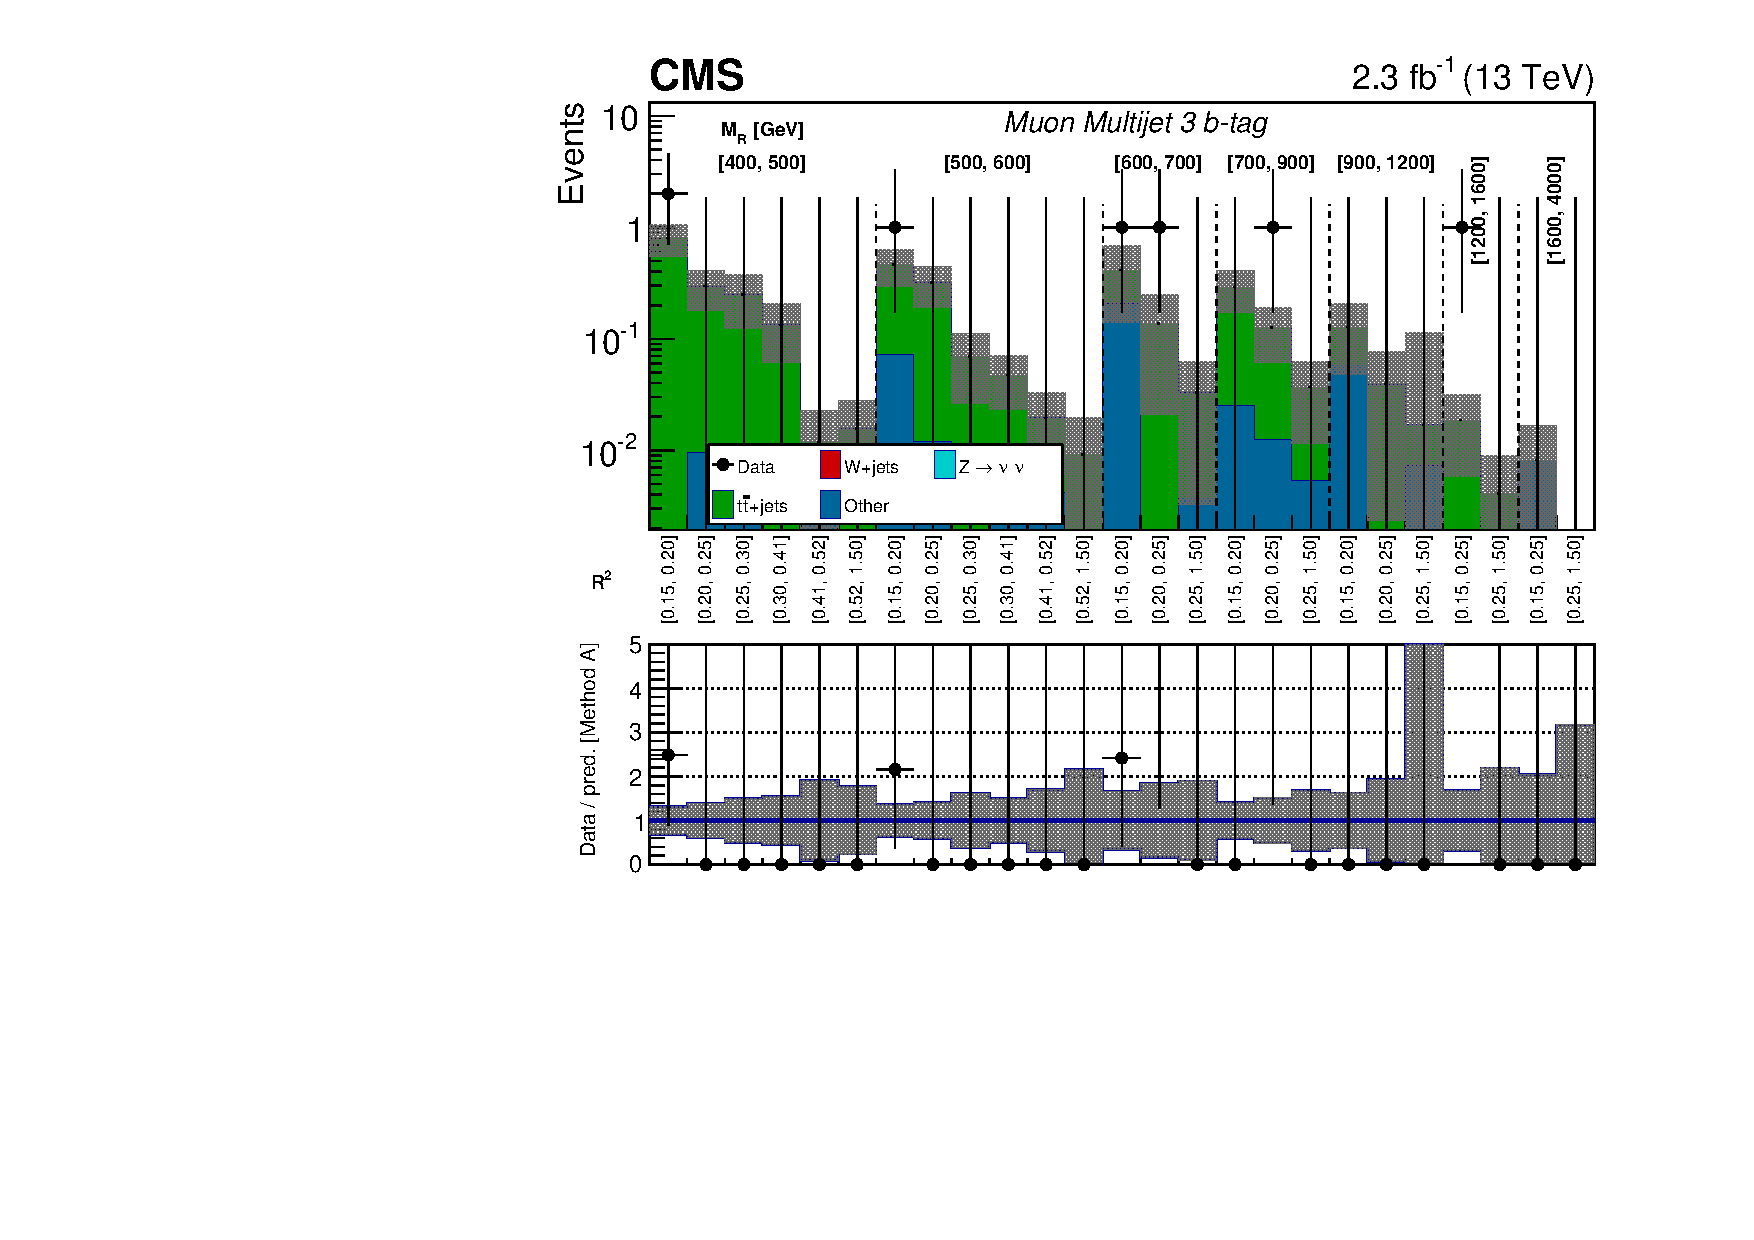
\includegraphics[width=0.8\textwidth]{figs/analysis13TeV/results/MRRsqMuMultiJet3BTagUnrolledDataMC.pdf}}
\caption{ The $\MR$-$\Rtwo$ distribution observed in data is shown along with the background prediction
obtained from method A for the Muon Multi-Jet event category in the 2 \PQb-tag (top) and $\geq 3$ \PQb-tag (bottom) bins. 
A detailed explanation of the plots is given in the caption of
  Figure~\ref{fig:ResultsMultiJet0btag1btag}.
}
\label{fig:ResultsMuMultiJet2btag3btag}
\end{figure}

\begin{figure}[!htb] \centering
\subfigure[0 \PQb-tag data]{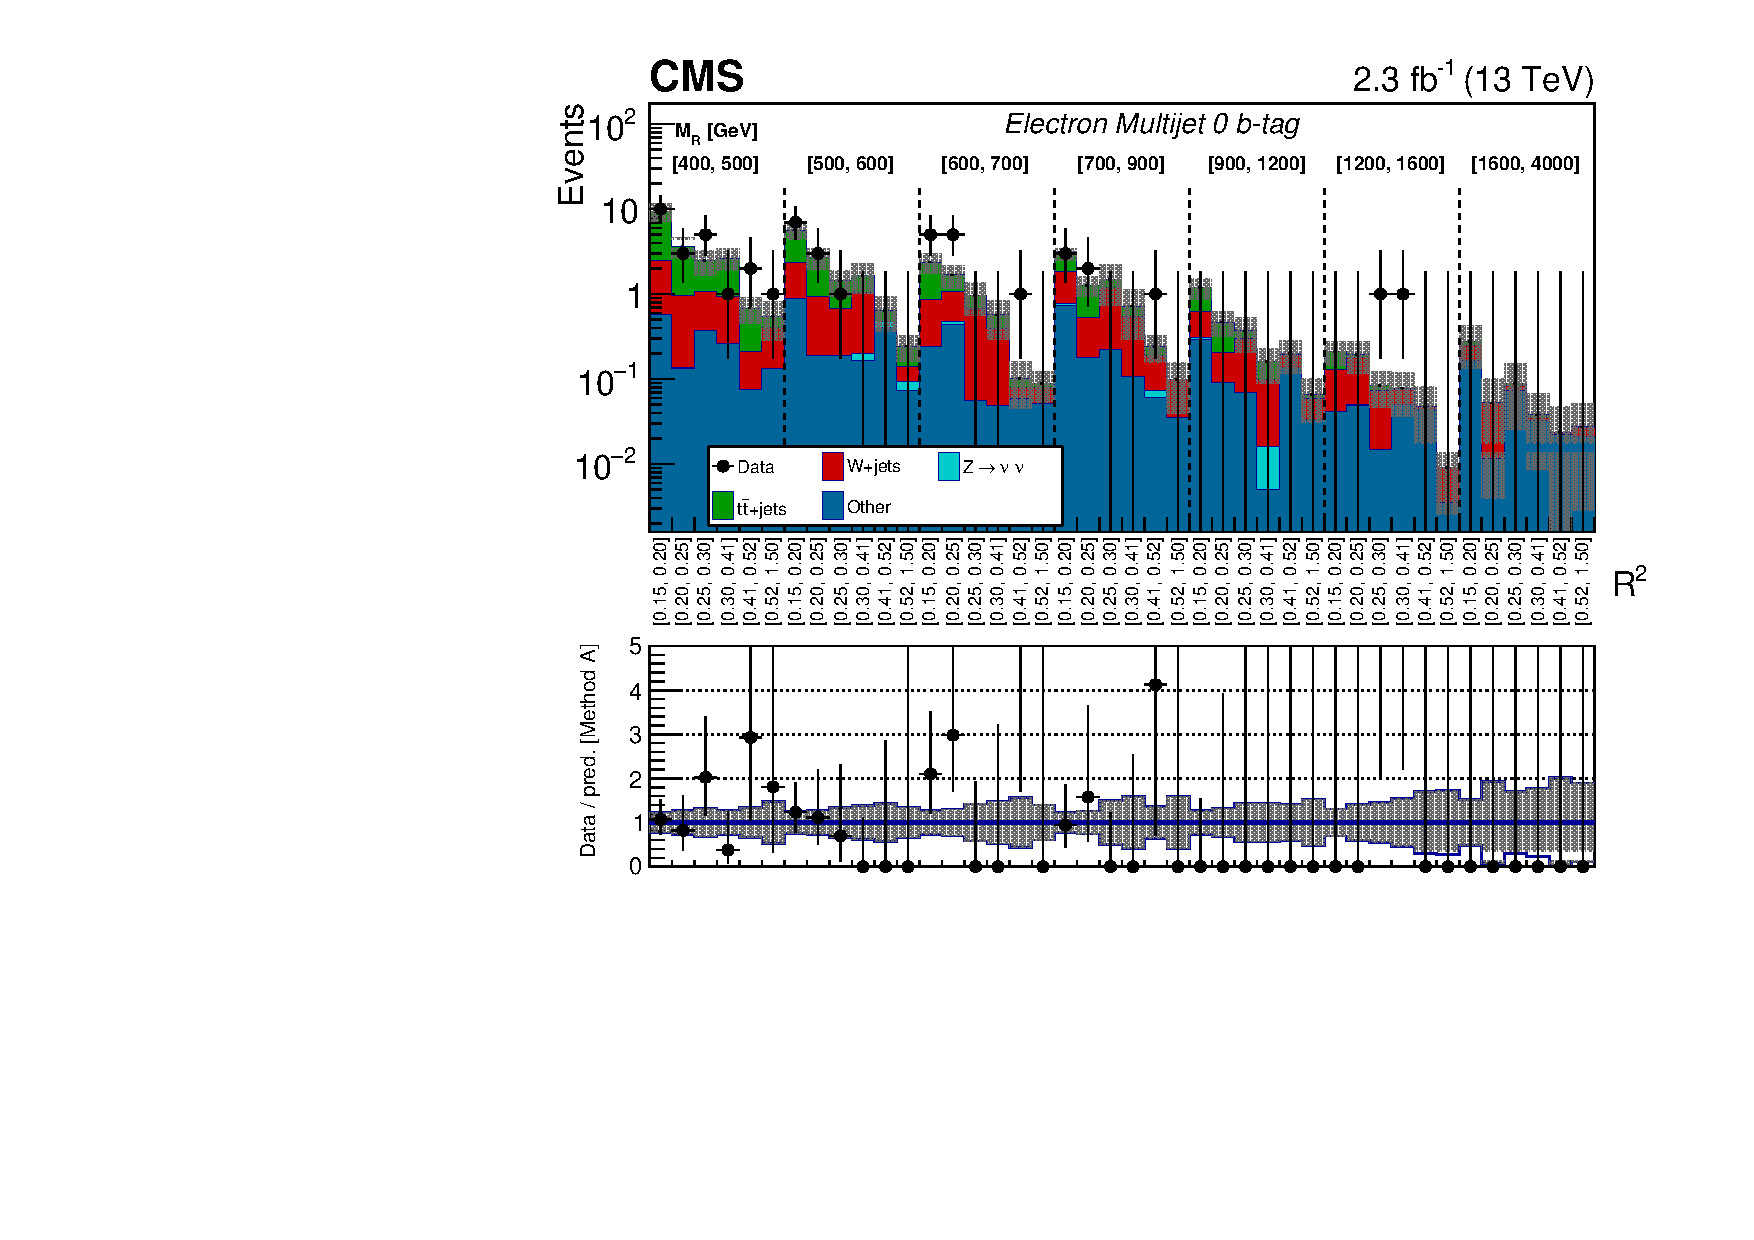
\includegraphics[width=0.8\textwidth]{figs/analysis13TeV/results/MRRsqEleMultiJet0BTagUnrolledDataMC.pdf}}\\
\subfigure[1 \PQb-tag data]{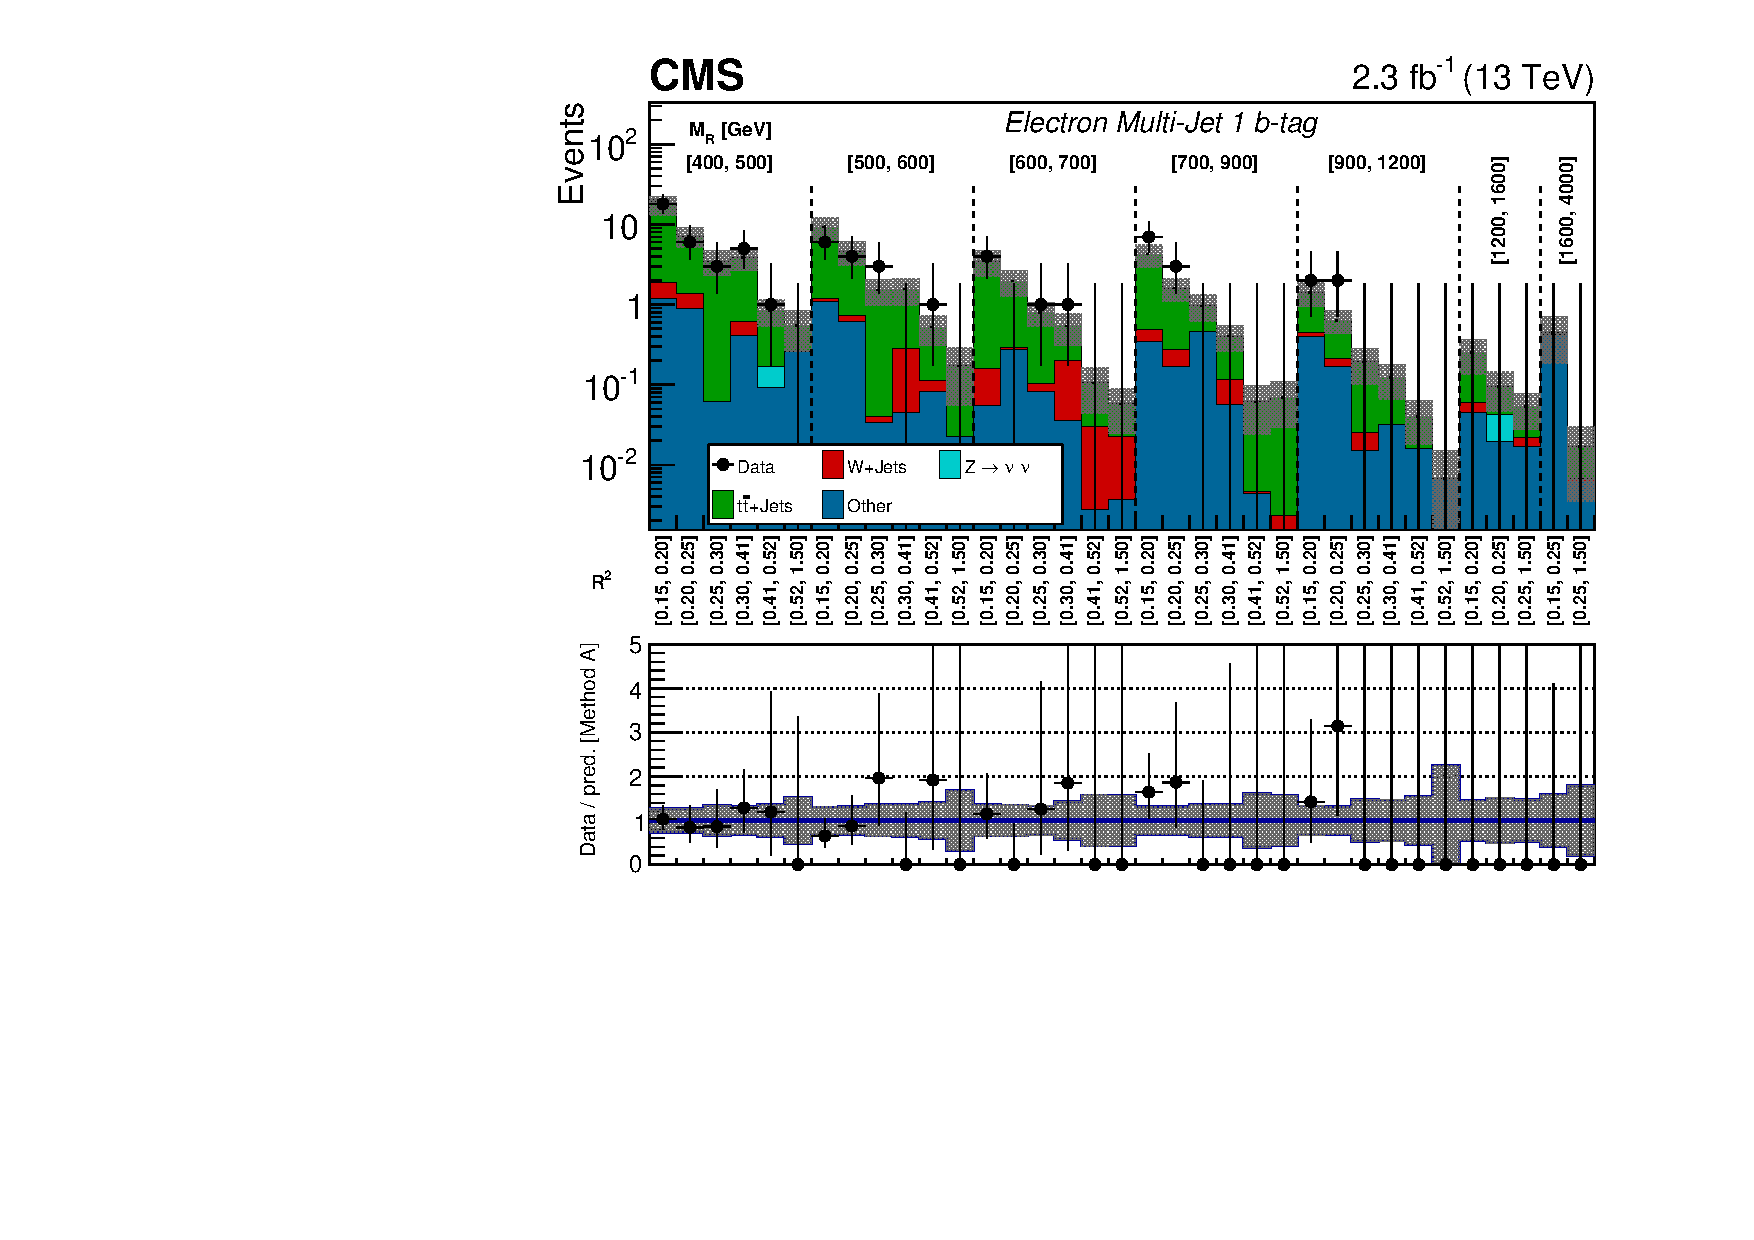
\includegraphics[width=0.8\textwidth]{figs/analysis13TeV/results/MRRsqEleMultiJet1BTagUnrolledDataMC.pdf}}
\caption{ The $\MR$-$\Rtwo$ distribution observed in data is shown along with the background prediction
obtained from method A for the Electron Multi-Jet event category in
the 0 \PQb-tag (top) and 1 \PQb-tag (bottom) bins. A detailed explanation of the plots is given in the caption of
  Figure~\ref{fig:ResultsMultiJet0btag1btag}.
}
\label{fig:ResultsEleMultiJet0btag1btag}
\end{figure}

\begin{figure}[!htb] \centering
\subfigure[2 \PQb-tag data]{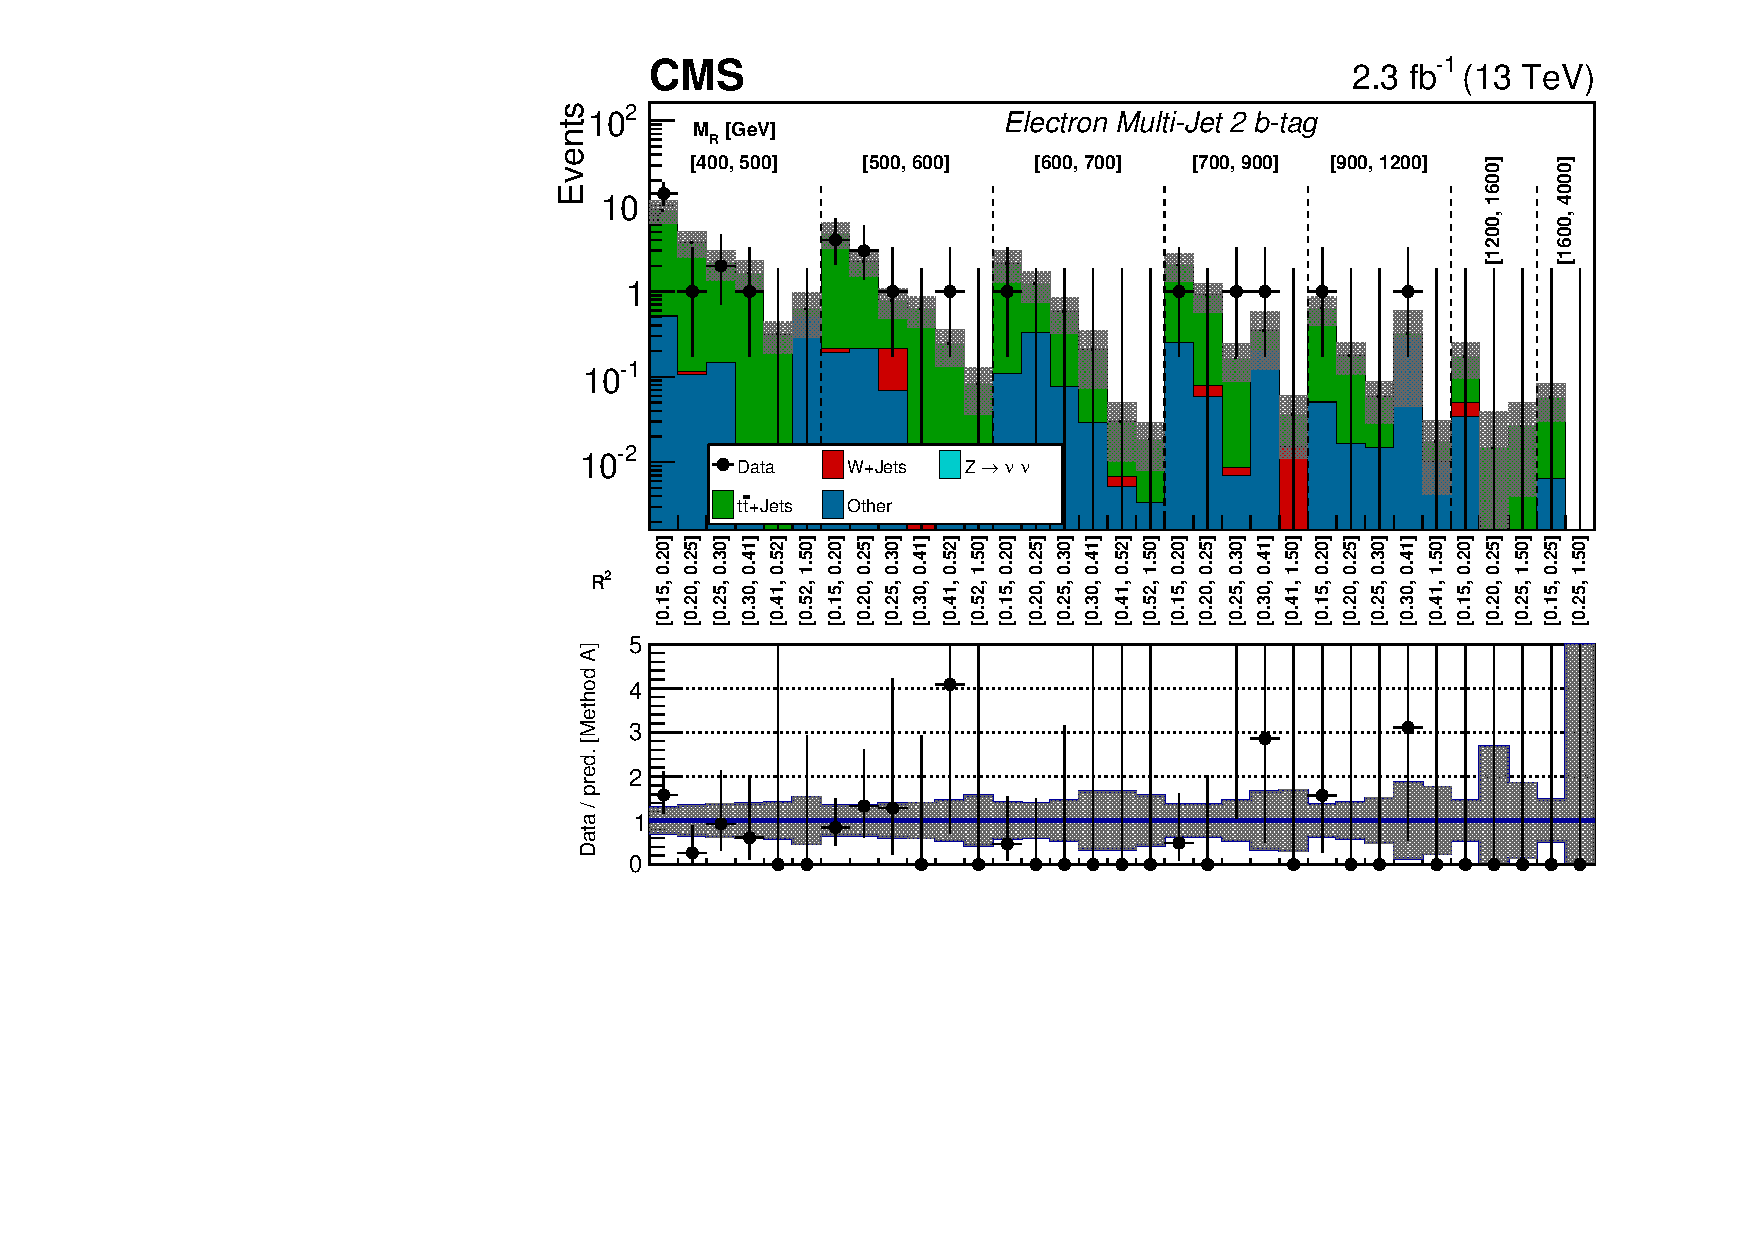
\includegraphics[width=0.8\textwidth]{figs/analysis13TeV/results/MRRsqEleMultiJet2BTagUnrolledDataMC.pdf}}\\
\subfigure[$\geq$ 3 \PQb-tag data]{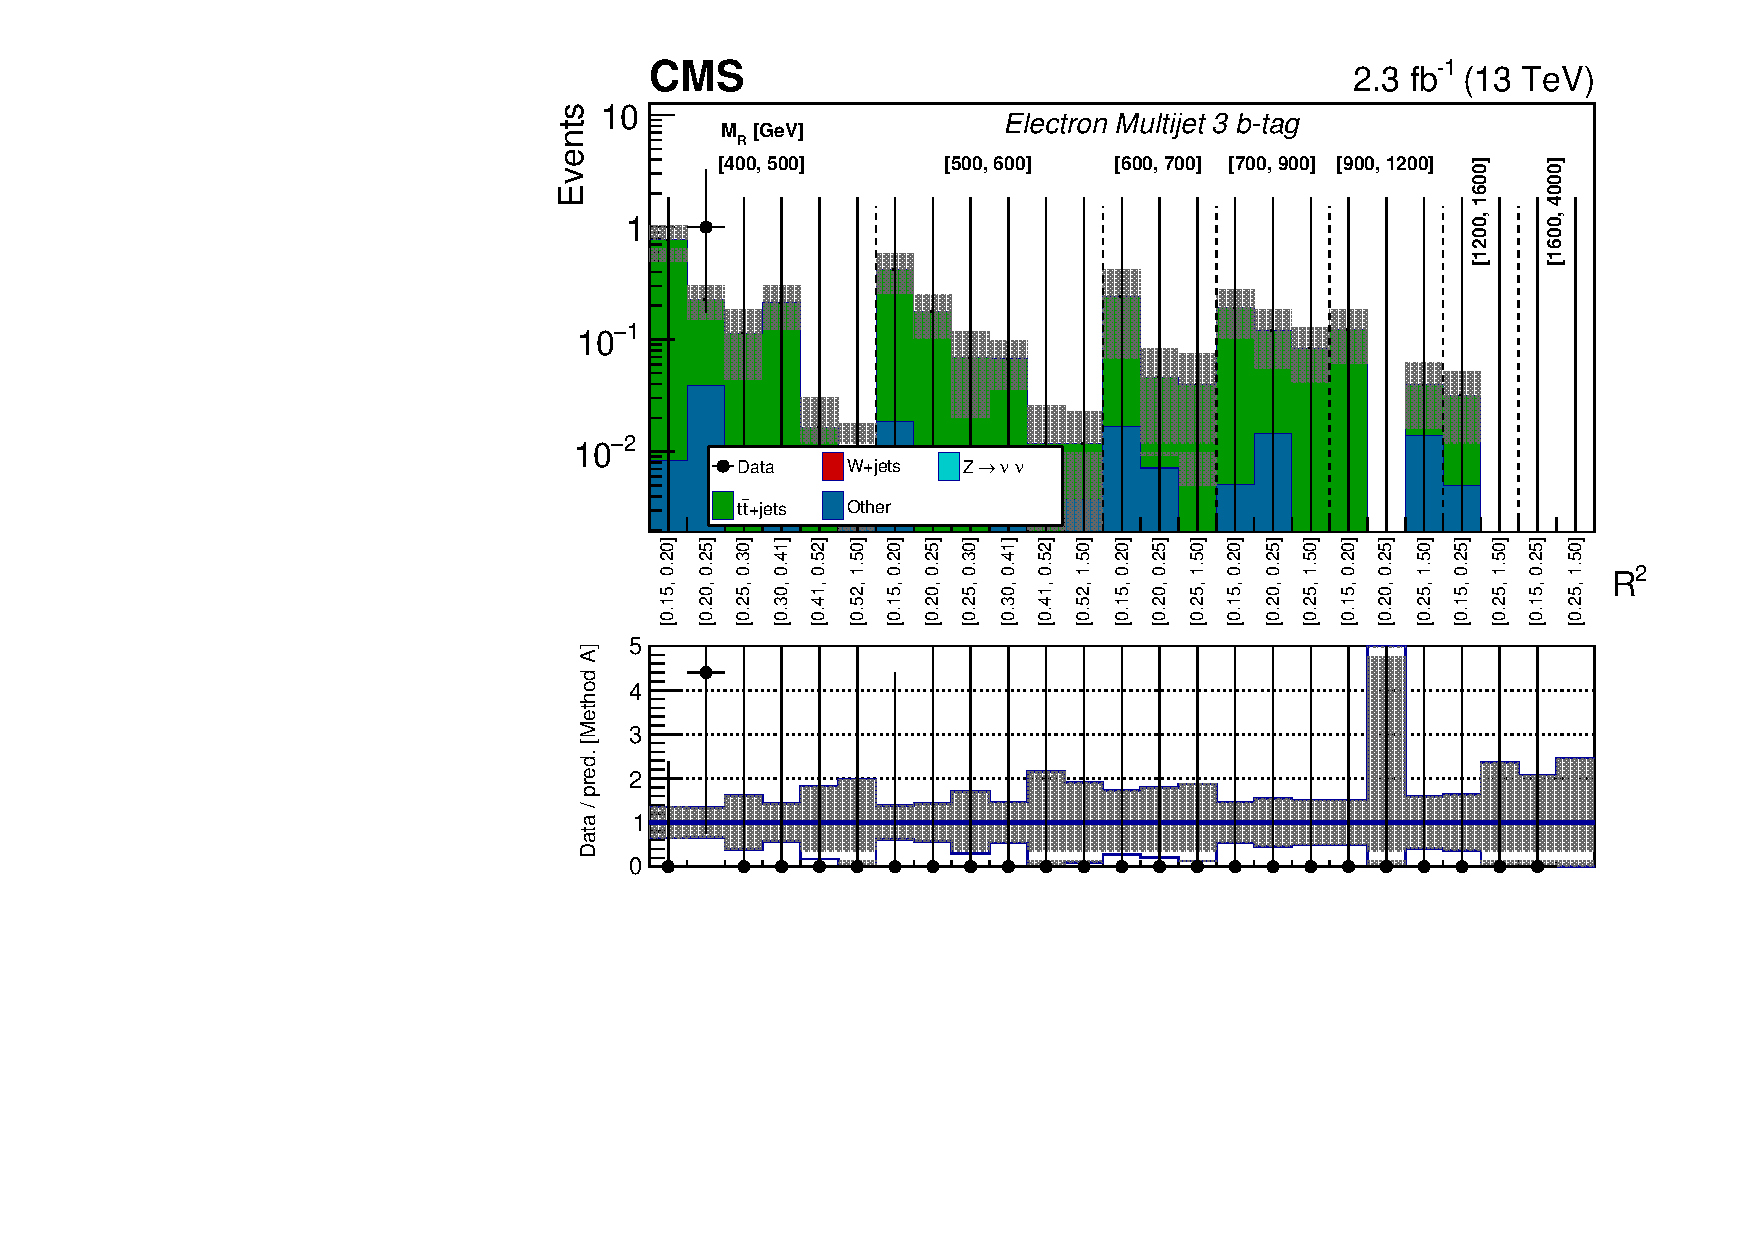
\includegraphics[width=0.8\textwidth]{figs/analysis13TeV/results/MRRsqEleMultiJet3BTagUnrolledDataMC.pdf}}
\caption{ The $\MR$-$\Rtwo$ distribution observed in data is shown along with the background prediction
obtained from method A for the Electron Multi-Jet event category in the 2 \PQb-tag (top) and $\geq 3$ \PQb-tag (bottom) bins. 
A detailed explanation of the plots is given in the caption of Figure~\ref{fig:ResultsMultiJet0btag1btag}.
}
\label{fig:ResultsEleMultiJet2btag3btag}
\end{figure}

\clearpage

First, we consider the scenario of gluino pair production
decaying to third generation quarks. The gluino decays to the third generation
are enhanced if the masses of the third generation squarks are
lighter than those of the first two generations, a scenario that is both theoretically and 
experimentally favored. Motivated by this, we consider the three decay
modes:
\begin{itemize}
\item $\PSg\rightarrow\bbbar\PSGcz$~;
\item $\PSg\rightarrow\ttbar\PSGcz$~; 
\item $\PSg\rightarrow\cPqb\cPaqt\chip\rightarrow\cPqb\cPaqt \PW^{\ast
    +}\PSGcz$~or~$\PSg\rightarrow\cPaqb\cPqt\chim\rightarrow\cPaqb\cPqt \PW^{\ast
    -}\PSGcz$~.
\end{itemize}

We perform a scan over all possible branching ratios to these three decay modes 
and compute limits on the production cross section under each such scenario. The production cross section
limits for a few characteristic branching ratio scan points are shown on the left of 
Figure~\ref{fig:GluinoToThirdGenLimits} as a function of the gluino and neutralino masses. We find a range of excluded regions
for different branching ratio assumptions and generally observe the strongest limits for
the $\PSg\rightarrow\bbbar\PSGcz$ decay mode over the full two-dimensional mass plane
and the weakest limits for the $\PSg\rightarrow\ttbar\PSGcz$ decay
mode. For scenarios that include the intermediate decay
$\chipm\to\PW^{\ast \pm}\PSGcz$ and small values of $m_{\chiz_1}$ the sensitivity
is reduced because the LSP carries very little momentum in both the
NLSP rest frame and the laboratory frame, resulting in small values of
$\ETmiss$ and $\Rtwo$. By considering the limits obtained for all scanned branching ratios, we
calculate the exclusion limits independent of any assumption of the branching
ratios, presented on the right of Figure~\ref{fig:GluinoToThirdGenLimits}. For
an LSP with mass of a few hundred $\GeV$, we exclude pair production of gluinos decaying 
to third generation quarks for mass below about $1600 \GeV$. This result 
represents a unique attempt at deriving a branching-ratio-independent limit on
gluino pair production at the LHC.


\begin{figure}[!htb] \centering
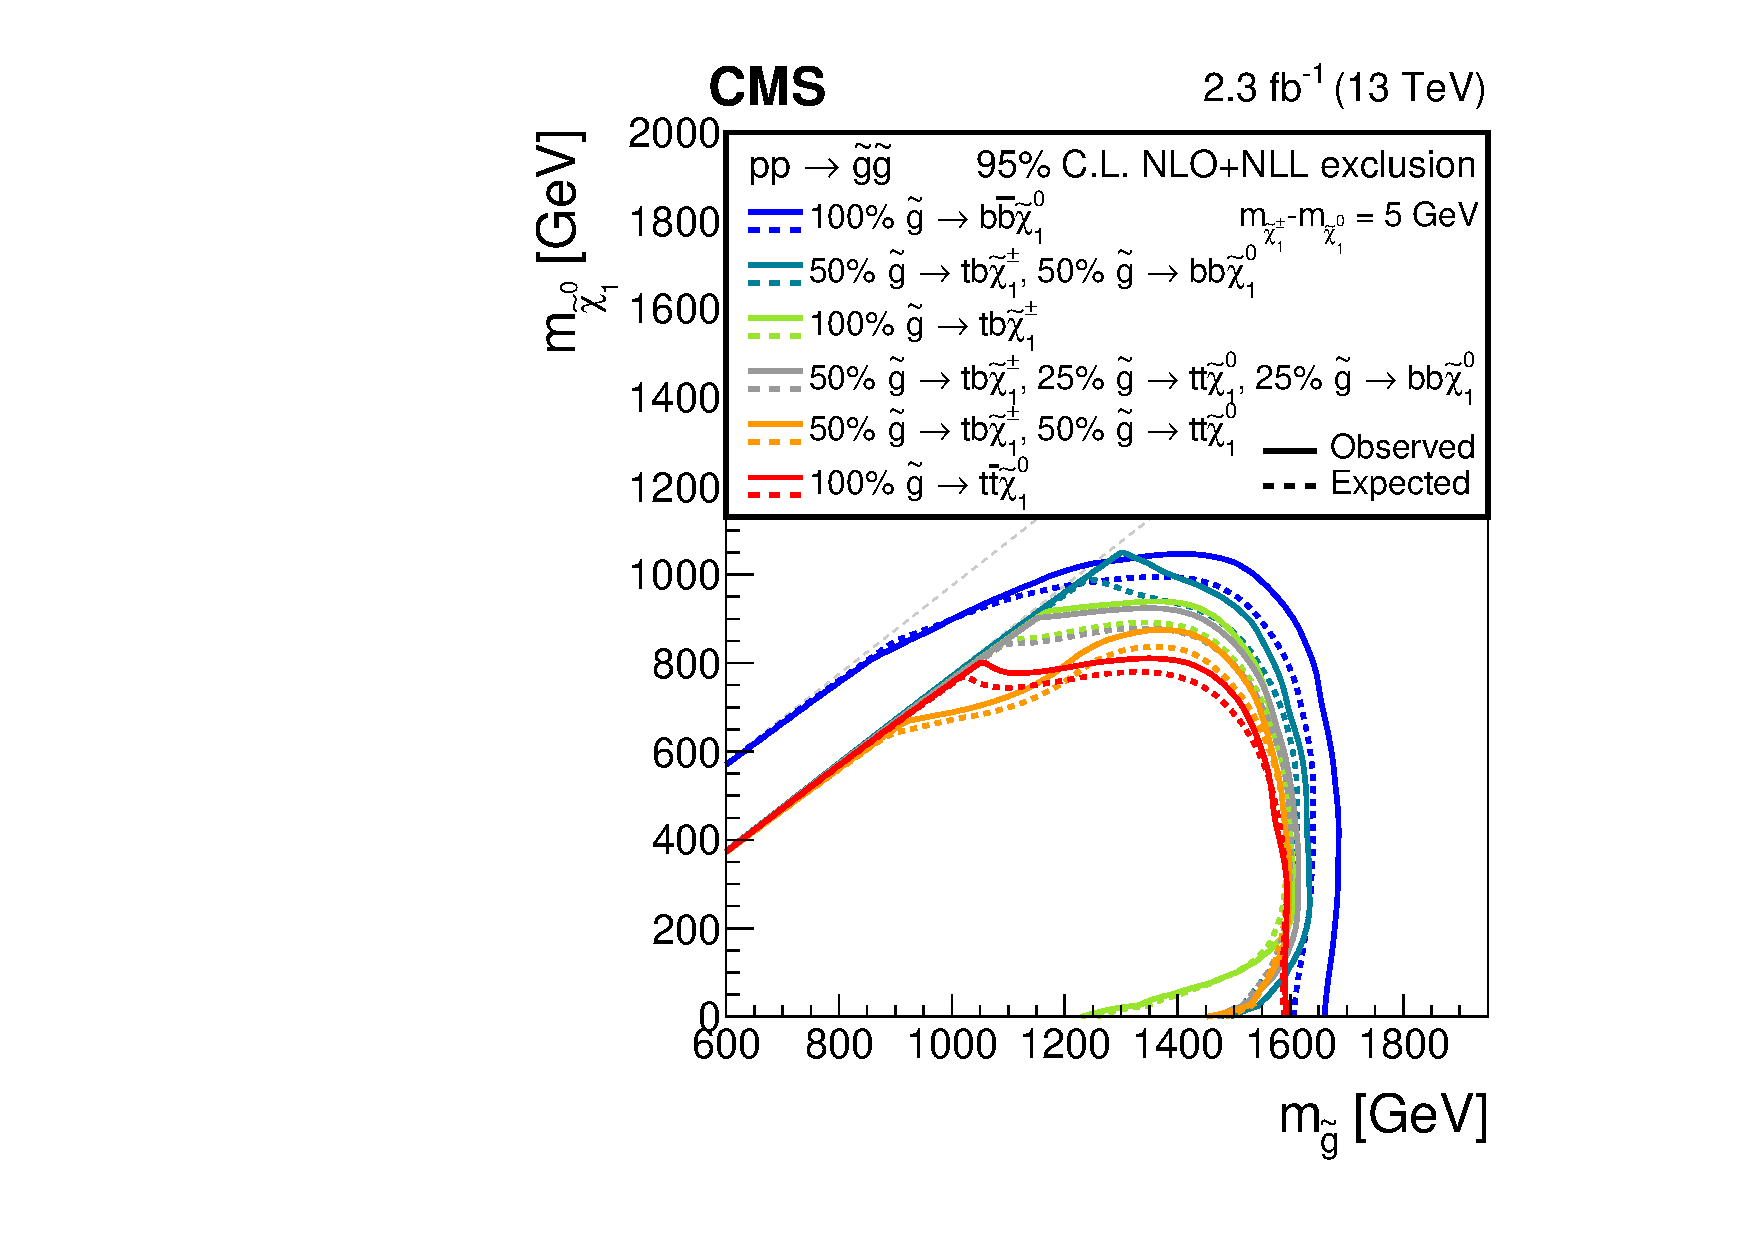
\includegraphics[width=0.49\textwidth]{figs/analysis13TeV/UnblindedResults/T1AsymptoticMADD.pdf}
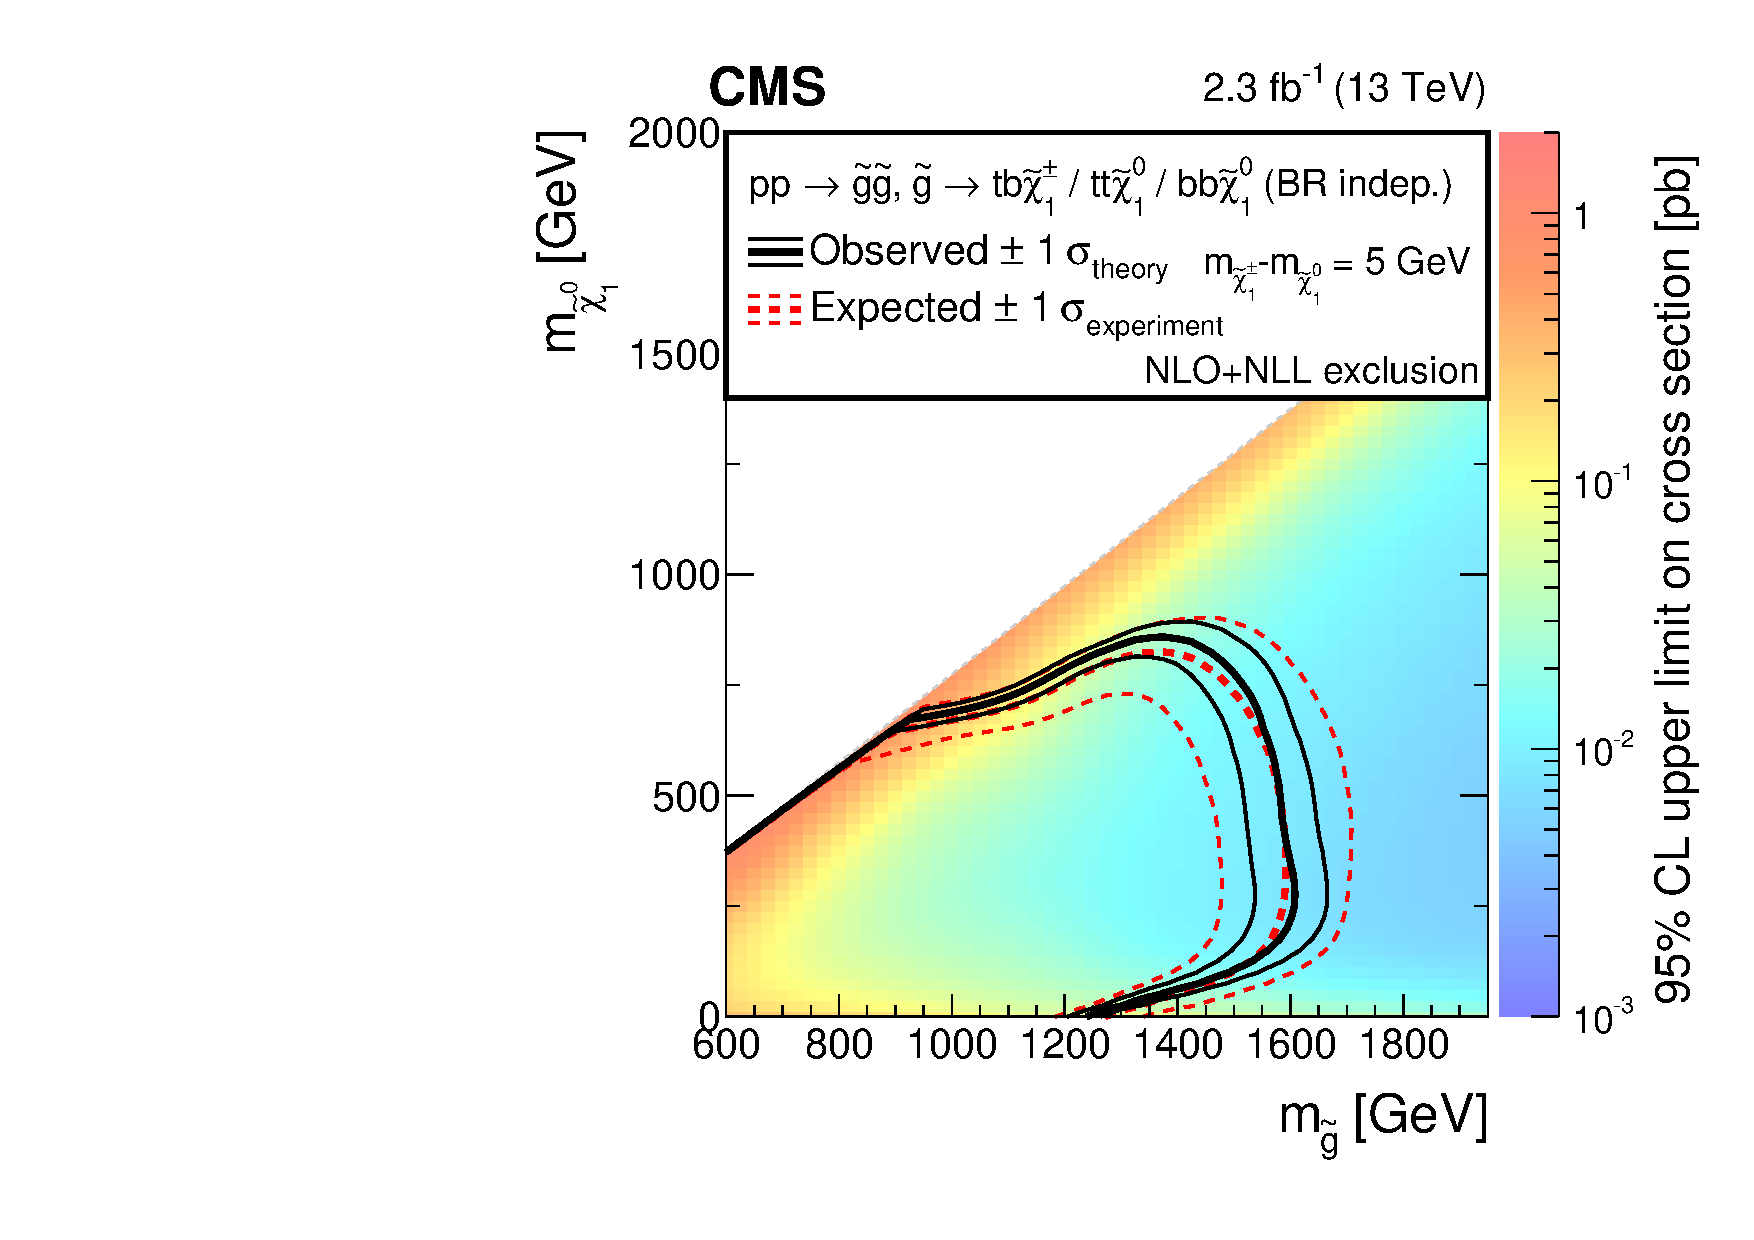
\includegraphics[width=0.49\textwidth]{figs/analysis13TeV/UnblindedResults/T1briFinalXSEC.pdf}
\caption{ On the left, we show the expected and observed 95\% upper limits on the production 
cross section for gluino pair production decaying to third generation quarks under various 
assumptions of the branching ratios. On the right, we show the analogous upper limits on 
the gluino pair production cross section independent of the gluino
decay branching ratios.
}
\label{fig:GluinoToThirdGenLimits}
\end{figure}


In Figure~\ref{fig:limitT1qqqqT2tt}, we present additional interpretations for
simplified model scenarios of interest. On the left, we show the production cross section
limits on gluino pair production where the gluino decays to two light flavored
quarks and the LSP, and on the right we show the production cross section limits on
top squark pair production where the top squark decays to a top quark and the LSP. 
For a very light LSP, we exclude top squark production with mass below
$750 \GeV$.

\begin{figure}[!htb] \centering
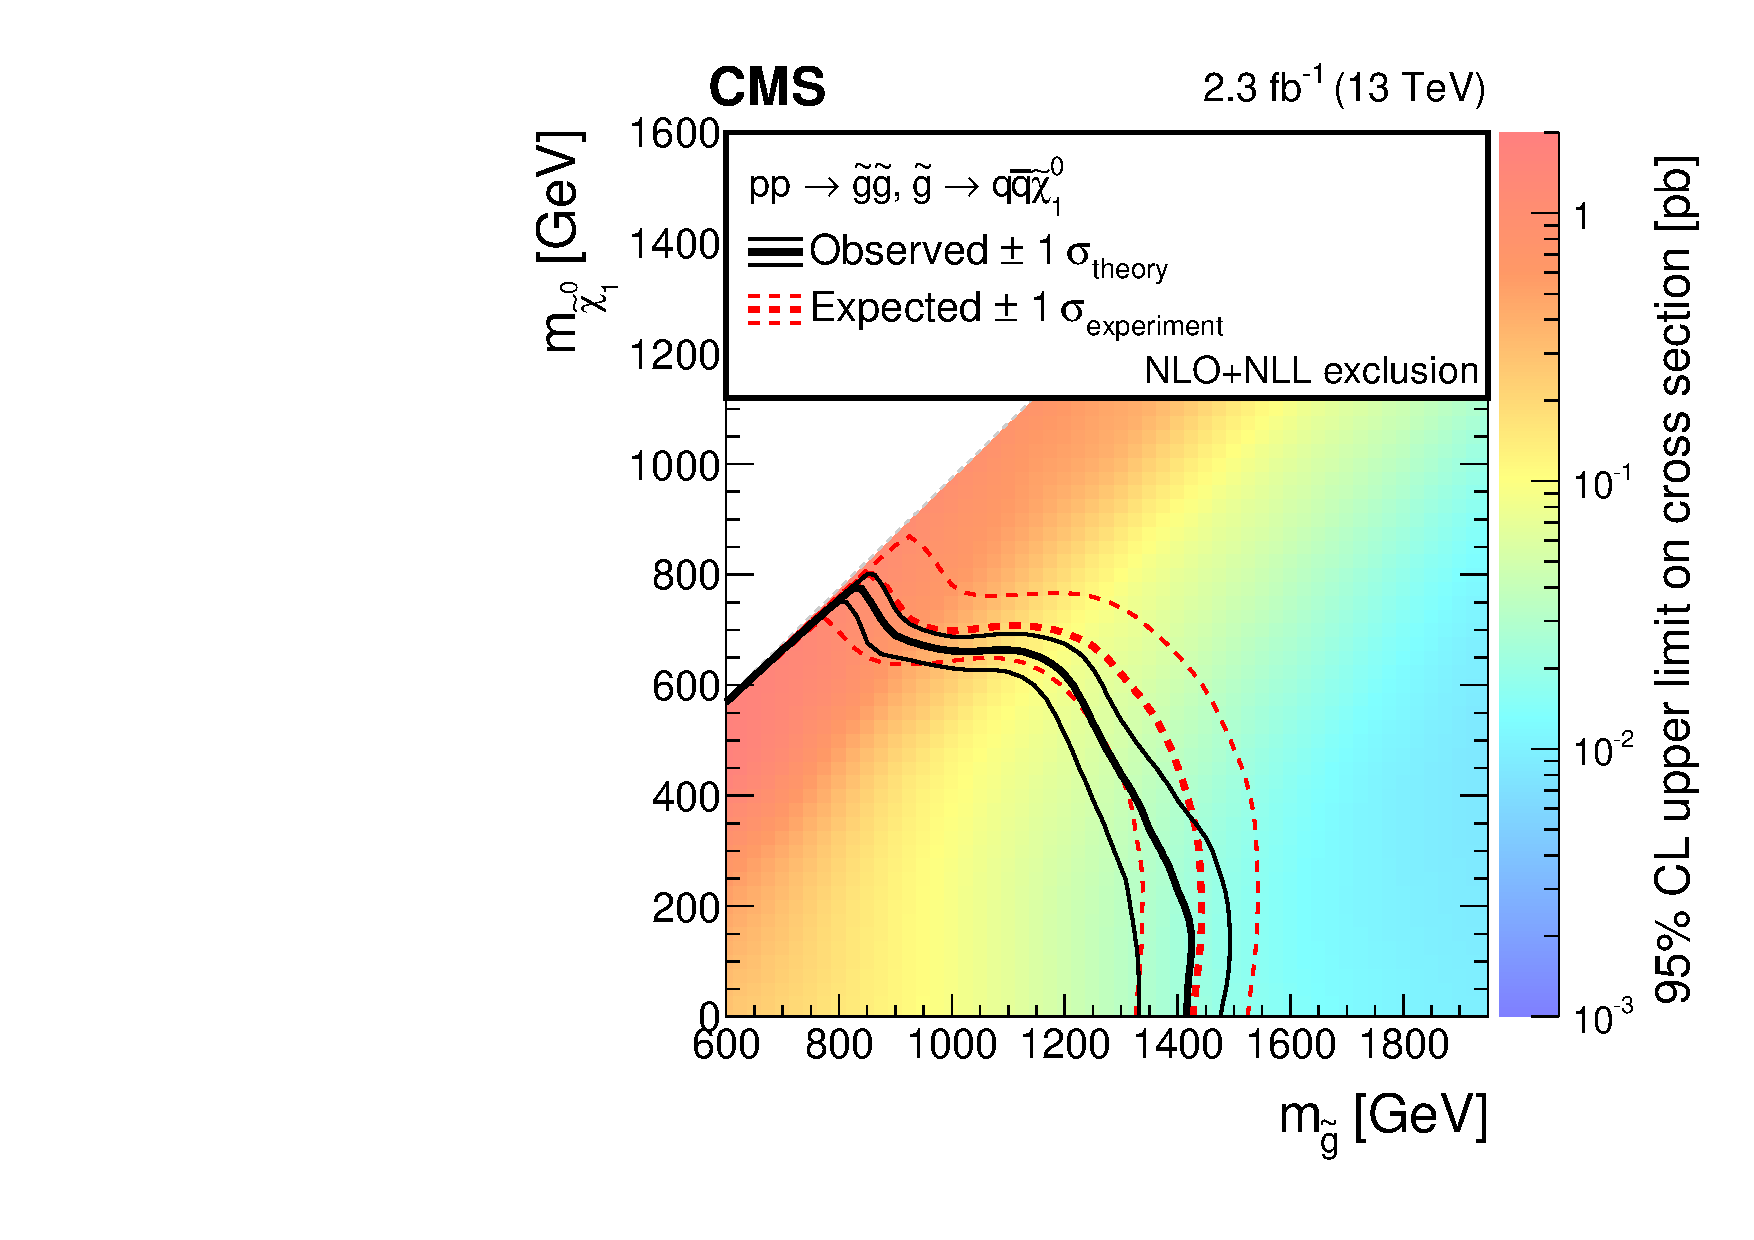
\includegraphics[width=0.49\textwidth]{figs/analysis13TeV/UnblindedResults/T1qqqqFinalXSEC.pdf}
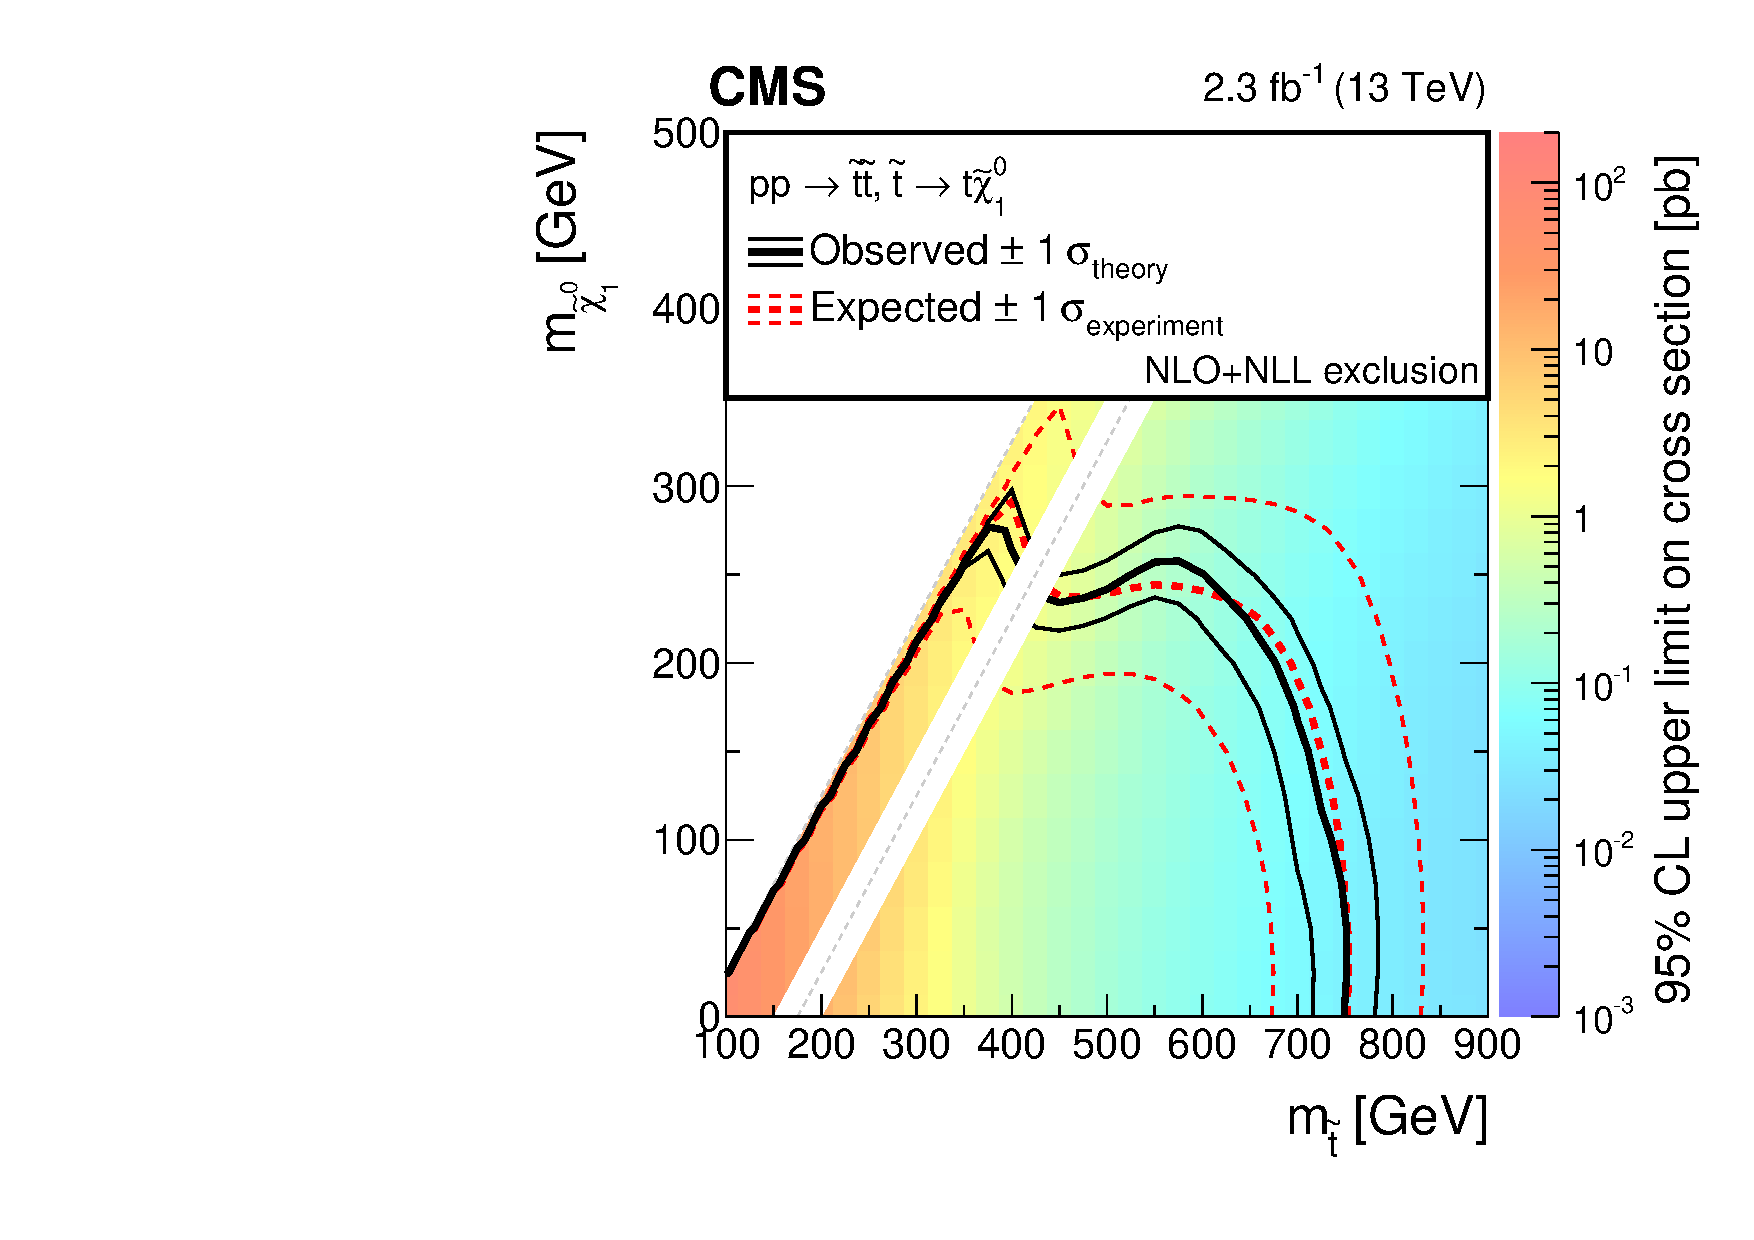
\includegraphics[width=0.49\textwidth]{figs/analysis13TeV/UnblindedResults/T2ttFinalXSEC.pdf}
\caption{ Expected and observed 95\% upper limits on the production cross section
for (left) gluino pair production decaying to two light flavored quarks and the LSP
and (right) top squark pair production decaying to a top quark and the LSP. 
The white diagonal band in the right plot corresponds to the region
$\abs{m_{\sTop}-m_{\PQt}-m_{\chiz_1}} < 25 \GeV$, where the signal 
efficiency is a strong function of $m_{\sTop}-m_{\chiz_1}$, and as a 
result the precise determination of the cross section upper limit is uncertain
because of the finite granularity of the available MC samples 
in this region of the ($m_{\sTop}$, $m_{\chiz_1}$)  plane.
}
\label{fig:limitT1qqqqT2tt}
\end{figure}


\section{Summary}
\label{sec:Summary}

We have presented an inclusive search for supersymmetry in events 
with no more than one lepton, a large multiplicty of energetic jets, and 
evidence of invisible particles. The search is sensitive to a broad
range of SUSY scenarios including pair production of gluinos and top
squarks, and the event categorization in the number of leptons and 
the number of \PQb-tagged jets enhances the signal to background and search
sensitivity simultaneously for a variety of different SUSY signal scenarios. 
We presented two alternative background estimation methods with very
different systematic assumptions, one relying on the applicability
of the simulation corrections derived in the control regions to the search regions, and 
the other relying on the accuracy of an assumed functional form dependence 
for the shape of background distribution in the $\MR$ and $\Rtwo$ variables.
We demonstrated that the two predictions agree to within their uncertainties, 
thereby significantly enhancing the robustness of the background modelling. 

No significant deviations from the predicted Standard Model background were
observed in any of the search regions, and this result is interpreted
in the context of simplified models of gluino or top
squark pair production. By scanning over all possible branching ratios
for gluino decays to third generation quarks, we derived exclusion
limits on gluino pair production that are independent of the gluino
decay branching ratios, representing a more generic constraint on 
gluino production than previously reported at the LHC. 
For an LSP with mass in the range between $200$ and $600$\GeV, we exclude gluinos
with mass below $1.55$ to $1.6$\TeV, independent of their decays.
For an LSP with a mass of $100$\GeV, we exclude top squarks below $750 \GeV$. 

